%======================================================================
% CHAPTER 4 — RELEASE 2: BI INFRASTRUCTURE
% Skeleton aligned with supervisor-approved NotMyChapitre4 structure
% Content: ATB Customer Risk BI platform (Airbyte → dbt → PFE_DWH → Streamlit)
%======================================================================
\chapter{Release 2: Design and Implementation of the Business Intelligence Infrastructure}
\label{chap:release2}

%----------------------------------------------------------------------
\section{Introduction}
%----------------------------------------------------------------------
If Release~1 concentrated on deploying a secure operational software architecture
and an autonomous orchestration engine, this Release~2 marks a
fundamental transition toward analytical steering. The exclusive objective of
this phase encapsulated in Sprint~3: Consult the BI Dashboard
is to design and deploy a complete Business Intelligence (BI) infrastructure for
the decision-makers of the Arab Tunisian Bank (ATB): Central General Management,
the Chief Compliance Officer and Branch Managers.

Building a decision-support system obeys conceptual paradigms distinct from
classical transactional software development. The agile Scrum framework,
although maintained for overall project management, was therefore hybridised
with a data-engineering methodology. It is in this context that we adopted the
GIMSI methodology.

This chapter traces the full journey from raw pipe-separated banking extracts
to an interactive, role-aware Streamlit dashboard, through a Kimball
constellation warehouse and a transparent three-pillar customer risk score.

%======================================================================
\section{Methodological Framework: GIMSI}
\label{sec:gimsi_framework}
%======================================================================

\subsection{Functional Specification and Use Case Diagram of Sprint~3}
Sprint~3 is entirely dedicated to the development and deployment of the
ATB Decision Dashboard. It is the convergence point of every prior
architectural decision: the Airbyte ingestion pipeline, the dbt ELT models and
the Kimball constellation warehouse all serve a single output in this iteration a polished, role-aware Streamlit application consumed in real-time by ATB
decision-makers.

The major objective of this sprint is to offer bank decision-makers an
interactive, modern and visual decision-support tool that facilitates strategic
monitoring of customer risk, portfolio balances and regulatory compliance
alerts. Unlike traditional static reports, the dashboard evolves dynamically
with each nightly Airflow refresh, ensuring that every KPI card, chart and
compliance flag reflects yesterday's warehouse snapshot rather than last
month's Excel extract.

To frame the deliverables of this sprint and guarantee alignment with the
supervisors' expectations, we formulated a complete functional specification
before writing a single line of Streamlit code. This specification process
involved three structured steps. First, we identified the three actor profiles
Central General Management, the Chief Compliance Officer and Branch
Managers and documented their distinct analytical needs. Second, we
translated those needs into user stories (US~04 to US~09) and organised them
into a sprint backlog with priority ratings. Third, we validated the scope with
UML modelling, producing the use-case diagram presented hereafter
(Figure~\ref{fig:use_case_sprint3}), which serves as the contractual interface
between the development team and the stakeholders throughout the sprint.

This phase concentrates on exploiting and valorising the decision data
consolidated in the data warehouse during the preceding ELT phase. Through the
Streamlit application interface, each authorised user benefits from an overview
of portfolio activity via dynamic Plotly charts and Key Performance Indicators
(KPIs) computed directly from the warehouse facts. Role-based access control
(RBAC) ensures that Branch Managers operate in a strictly scoped view of their
own Desk Account Officer perimeter, while Central General Management retains a
cross-agency, national panorama.

With the functional scope fully specified and version-controlled, we can now
detail the interactions formalised in the use-case diagram below
(Figure~\ref{fig:use_case_sprint3}), which covers every actor and primary
behaviour supported during Sprint~3:

\begin{figure}[H]
\centering
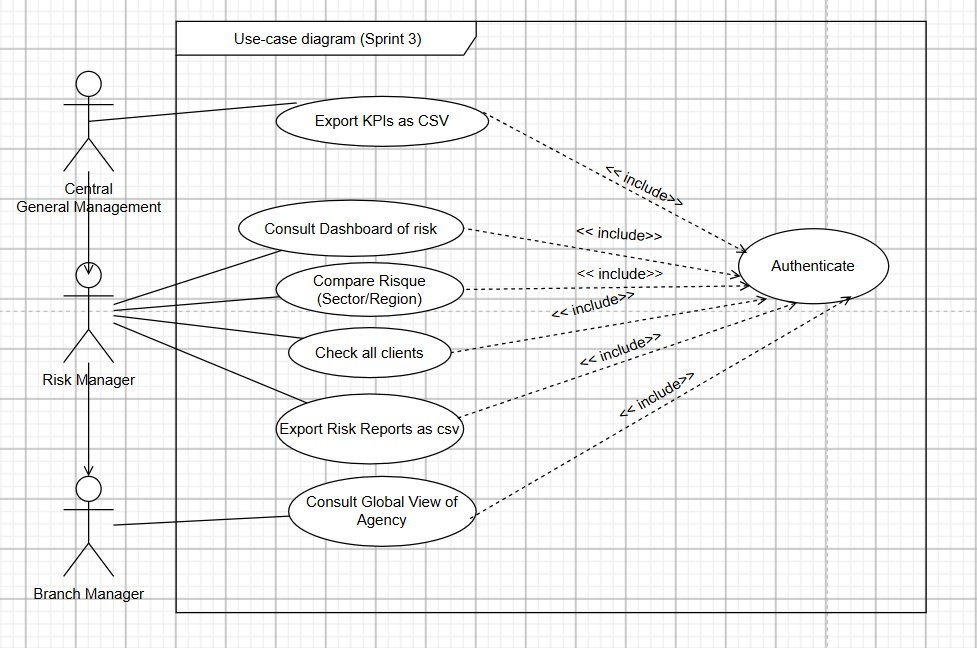
\includegraphics[width=0.9\textwidth]{figures/DiagramUseCaseSprint3.png}
\caption{Use-case diagram of the ATB Decision Dashboard (Sprint~3)}
\label{fig:use_case_sprint3}
\end{figure}

As illustrated, every actor interacts with the principal use case
\textbf{Consult the BI Dashboard}. Access requires authentication
(\textit{include}). Once connected, extended behaviours deepen the analysis:
\begin{itemize}
    \item \textbf{Visualisation of strategic KPIs:} synthetic follow-up of portfolio
          health (balances, average risk, overdraft rate).
    \item \textbf{Visualisation of Plotly charts:} dynamic exploration of risk tiers,
          sectors, industries and branches.
    \item \textbf{Branch-scoped filtering:} DAO restriction for Branch Managers
          (US~06).
    \item \textbf{Compliance watchlists:} PEP / KYC / flag queues for the Chief
          Compliance Officer.
    \item \textbf{AI chart explanations:} Gemini-generated textual readings with a
          deterministic template fallback.
    \item \textbf{Export of audit packs:} CSV and PDF extraction for committees
          (US~08).
\end{itemize}

Table~\ref{tab:sprint3_backlog} recalls the Sprint~3 product backlog (US~04 to
US~09) already defined in Chapter~2.

\begin{table}[H]
\centering
\caption{Product Backlog for Sprint~3 (Release~2)}
\label{tab:sprint3_backlog}
\renewcommand{\arraystretch}{1.35}
\resizebox{\textwidth}{!}{%
\begin{tabular}{|c|c|p{3.0cm}|p{5.6cm}|p{4.0cm}|}
\hline
\rowcolor{blue!15}
\textbf{ID} & \textbf{Priority} & \textbf{As a\ldots} & \textbf{I want to\ldots} & \textbf{So that\ldots} \\
\hline
\textbf{US 04} & High & Central GM & extract and load sources via Airbyte & ODS is fed without manual copy. \\
\hline
\textbf{US 05} & High & Central GM & define and calculate risk KPIs in the DWH & portfolio health uses shared audited formulas. \\
\hline
\textbf{US 06} & High & Branch Manager & consult my agency's filtered Streamlit view & I monitor local risk without seeing other branches. \\
\hline
\textbf{US 07} & High & Central GM & analyse indicators for all agencies nationally & I compare regions and risk concentrations. \\
\hline
\textbf{US 08} & High & Central GM & export management indicators as CSV/PDF & audit packs can leave the tool. \\
\hline
\textbf{US 09} & Low & Risk Manager & track customer history across agencies & score evolution remains visible over time. \\
\hline
\end{tabular}%
}
\end{table}

\subsection{Application of GIMSI to Sprint~3}
To meet Release~2 requirements, the software architecture of the platform was
rigorously mapped onto the four GIMSI pillars. Table~\ref{tab:gimsi_phases}
illustrates the exact cartography between the theoretical GIMSI framework, BI
architecture concepts and the technical implementations realised in this sprint.
Figure~\ref{fig:gimsi_cycle_atb} summarises the cycle graphically.

\begin{figure}[H]
\centering
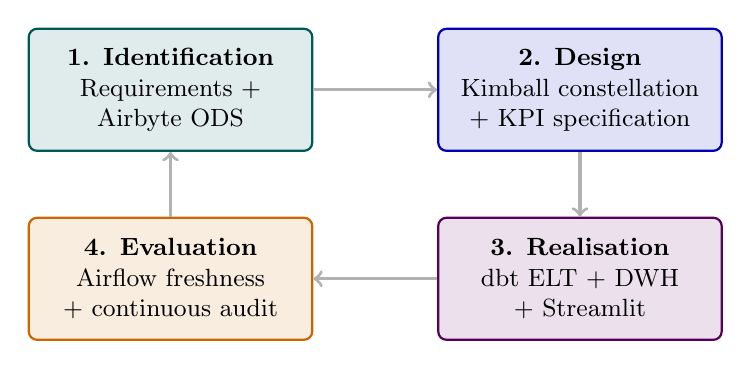
\begin{tikzpicture}[
  font=\small,
  phase/.style={rectangle, rounded corners=3pt, draw=#1, fill=#1!12, thick,
                align=center, minimum width=3.6cm, minimum height=1.55cm},
  arr/.style={->, very thick, gray!60}
]
  \node[phase=teal!70!black] (p1) at (0,2.4) {\textbf{1. Identification}\\Requirements +\\Airbyte ODS};
  \node[phase=blue!70!black] (p2) at (5.2,2.4) {\textbf{2. Design}\\Kimball constellation\\+ KPI specification};
  \node[phase=violet!70!black] (p3) at (5.2,0.0) {\textbf{3. Realisation}\\dbt ELT + DWH\\+ Streamlit};
  \node[phase=orange!80!black] (p4) at (0,0.0) {\textbf{4. Evaluation}\\Airflow freshness\\+ continuous audit};
  \draw[arr] (p1) -- (p2);
  \draw[arr] (p2) -- (p3);
  \draw[arr] (p3) -- (p4);
  \draw[arr] (p4) -- (p1);
\end{tikzpicture}
\caption{GIMSI cycle applied to the ATB BI Release~2}
\label{fig:gimsi_cycle_atb}
\end{figure}

\begin{table}[H]
\centering
\caption{Cartography of the GIMSI methodology applied to the ATB BI architecture}
\label{tab:gimsi_phases}
\renewcommand{\arraystretch}{1.25}
\scriptsize
\begin{tabular}{|p{2.6cm}|p{4.0cm}|p{7.4cm}|}
\hline
\rowcolor{blue!15}
\textbf{GIMSI Phase} & \textbf{BI Architecture Concept} & \textbf{Implementation in Sprint~3} \\
\hline
\textbf{1. Identification} & Requirements model \& source acquisition & Actors DG / Compliance / Branch; FR/NFR; seven pipe-separated CSVs synchronised by Airbyte into \texttt{PFE\_ODS}. \\
\hline
\textbf{2. Design} & Dimensional modelling & Kimball constellation (8 dimensions + 2 facts); mathematical definition of portfolio and risk KPIs; visual dashboard specification. \\
\hline
\textbf{3. Realisation} & Access, Warehouse, Business \& Presentation layers & dbt ELT (staging / intermediate / warehouse), three-pillar scoring, SQL Server \texttt{PFE\_DWH}, Streamlit RBAC dashboard. \\
\hline
\textbf{4. Evaluation} & Freshness \& continuous improvement & Airflow nightly schedule (\texttt{0 2 * * *}), Streamlit TTL cache, dbt tests, KPI evolution roadmap. \\
\hline
\end{tabular}
\end{table}

%======================================================================
\section{Phase 1: Identification}
\label{sec:gimsi_phase1}
%======================================================================
The first phase aims to understand the context, inventory dashboard requirements,
and identify and extract the raw data that will feed the warehouse.

\subsection{The Requirements Model}
The requirements model is a design artefact used to document the expectations of
ATB decision-makers. It clarified the functionalities that the BI layer must
deliver:
\begin{itemize}
    \item obtain instant visibility on portfolio balances and average customer risk;
    \item isolate profiles requiring urgent compliance or credit follow-up
          (PEP, incomplete KYC, high Global Risk Score);
    \item analyse distributions by sector, industry, employment and branch area;
    \item enforce branch segregation so that a local manager never sees another
          agency's book.
\end{itemize}

\paragraph{Identified actors.}
\begin{itemize}
    \item \textbf{Central General Management:} macroscopic
          national view, cross-agency comparison, export for committees.
    \item \textbf{Chief Compliance Officer:} KYC/PEP
          watchlists, compliance flags, alert inbox.
    \item \textbf{Branch Manager:} same analytical language,
          restricted to the Desk Account Officer (DAO) / branch perimeter.
\end{itemize}

\paragraph{Functional Requirements (FR).}
\begin{itemize}
    \item \textbf{FR1 --- Portfolio KPIs:} display aggregated indicators (customers,
          accounts, total balance, average risk, overdraft share).
    \item \textbf{FR2 --- Risk profiling:} compute a daily classification into
          \texttt{LOW} / \texttt{MEDIUM} / \texttt{HIGH} / \texttt{VERY\_HIGH}.
    \item \textbf{FR3 --- Branch segregation:} filter analytical outputs by DAO area
          for Branch Managers.
    \item \textbf{FR4 --- Watchlist audit:} expose PEPs, incomplete KYC and overdue
          review dates.
    \item \textbf{FR5 --- Detail inspection:} open a customer fiche with the
          three-pillar breakdown (CRI, FFS, BRS).
    \item \textbf{FR6 --- Explainable insights:} provide AI-generated chart
          explanations to support reading during committees.
\end{itemize}

\paragraph{Non-Functional Requirements (NFR).}
\begin{itemize}
    \item \textbf{NFR1 --- Row-level security:} SQL filters injected from the session
          (\texttt{dao\_filter\_sql()}).
    \item \textbf{NFR2 --- Render latency:} interactive pages respond in under
          $\approx 2$~s in normal use.
    \item \textbf{NFR3 --- Access efficiency:} SQLAlchemy connection pooling and
          Streamlit result caching.
    \item \textbf{NFR4 --- Referential integrity:} $100\%$ fact foreign keys resolved
          (sentinel UNKNOWN rows; zero NULL FKs).
    \item \textbf{NFR5 --- Traceability:} every transformation versioned in Git and
          covered by dbt tests.
\end{itemize}

Table~\ref{tab:fr_nfr_traceability} cross-references requirements to Sprint~3
user stories and technical components --- a traceability artefact required for
academic and audit readability.

\begin{table}[H]
\centering
\caption{Requirements-to-implementation traceability matrix}
\label{tab:fr_nfr_traceability}
\renewcommand{\arraystretch}{1.2}
\scriptsize
\begin{tabular}{|c|p{4.2cm}|c|p{5.5cm}|}
\hline
\rowcolor{blue!15}
\textbf{Req.} & \textbf{Intent} & \textbf{US} & \textbf{Technical realisation} \\
\hline
FR1 & Portfolio KPI cards & US~05, US~07 & \texttt{loaders.load\_executive\_kpis()} on \texttt{fact\_*} \\
\hline
FR2 & Daily risk tiers & US~05 & \texttt{int\_customer\_risk\_score} $\rightarrow$ \texttt{fact\_customer\_risk} \\
\hline
FR3 & Branch segregation & US~06 & RBAC + \texttt{dao\_filter\_sql()} \\
\hline
FR4 & PEP / KYC watchlists & US~05 & Compliance + Alert inbox pages \\
\hline
FR5 & Three-pillar fiche & US~05, US~09 & Risk page + \texttt{dim\_risk\_profile} \\
\hline
FR6 & AI explanations & US~07 & Gemini explainer + template fallback \\
\hline
NFR1 & Row-level security & US~06 & Session-scoped SQL WHERE \\
\hline
NFR4 & Zero NULL FKs & US~05 & Sentinel $-1$ / \texttt{UNK} + \texttt{COALESCE} \\
\hline
NFR5 & Tested lineage & US~04, US~05 & Airbyte $\rightarrow$ dbt tests $\rightarrow$ Airflow DQ \\
\hline
\end{tabular}
\end{table}

\subsection{Data Source Acquisition (Airbyte on Docker, Hosted via GitHub)}
In practice, a BI project is only as trustworthy as the way raw files enter the
system. ATB provided seven pipe-separated (\texttt{|}) CSV extracts from the core
banking environment. Rather than copying them by hand into SQL Server, we built
a small but realistic enterprise pattern: \textbf{publish the files once, sync
them automatically forever}.

\paragraph{GitHub as a Data Host}
The CSV extracts were published under the project repository path
\texttt{data/raw/}. GitHub then acts as a lightweight, versioned file host:
each raw file is reachable through a stable HTTPS raw URL that Airbyte can
poll. This choice has three practical advantages for a PFE deployment:
\begin{itemize}
    \item \textbf{Version control:} every change to a source extract is committed
          and auditable;
    \item \textbf{No local path fragility:} Airbyte does not depend on a Windows
          folder that may move or disappear;
    \item \textbf{Repeatable demos:} anyone with repository access can rebuild the
          same ingestion from the same published URLs.
\end{itemize}

\paragraph{Airbyte running in Docker.}
Airbyte itself is deployed as a \textbf{Docker} stack (containers for the web UI,
workers and temporal services). From the browser UI we created seven
\textbf{HTTPS / File} source connectors one per CSV pointing to those
GitHub raw URLs. For each connector we configured:
\begin{itemize}
    \item format \texttt{csv}, delimiter \texttt{|}, header row enabled;
    \item explicit column dtypes (strings for codes, floats for balances/salary);
    \item a destination dataset name in the ODS
          (\texttt{ODS\_CUSTOMER}, \texttt{ODS\_ACCOUNT}, \texttt{ODS\_DAO},\ldots).
\end{itemize}
The destination connector targets Microsoft SQL Server, schema
\texttt{PFE\_ODS}, database \texttt{ATB\_BI}. After a successful sync, the ODS
contains a faithful mirror of the GitHub files, enriched with Airbyte technical
columns such as \texttt{\_airbyte\_raw\_id} and \texttt{\_airbyte\_extracted\_at}.

Figure~\ref{fig:airbyte_ingest_flow} formalises this chain.
\begin{figure}[H]
\centering
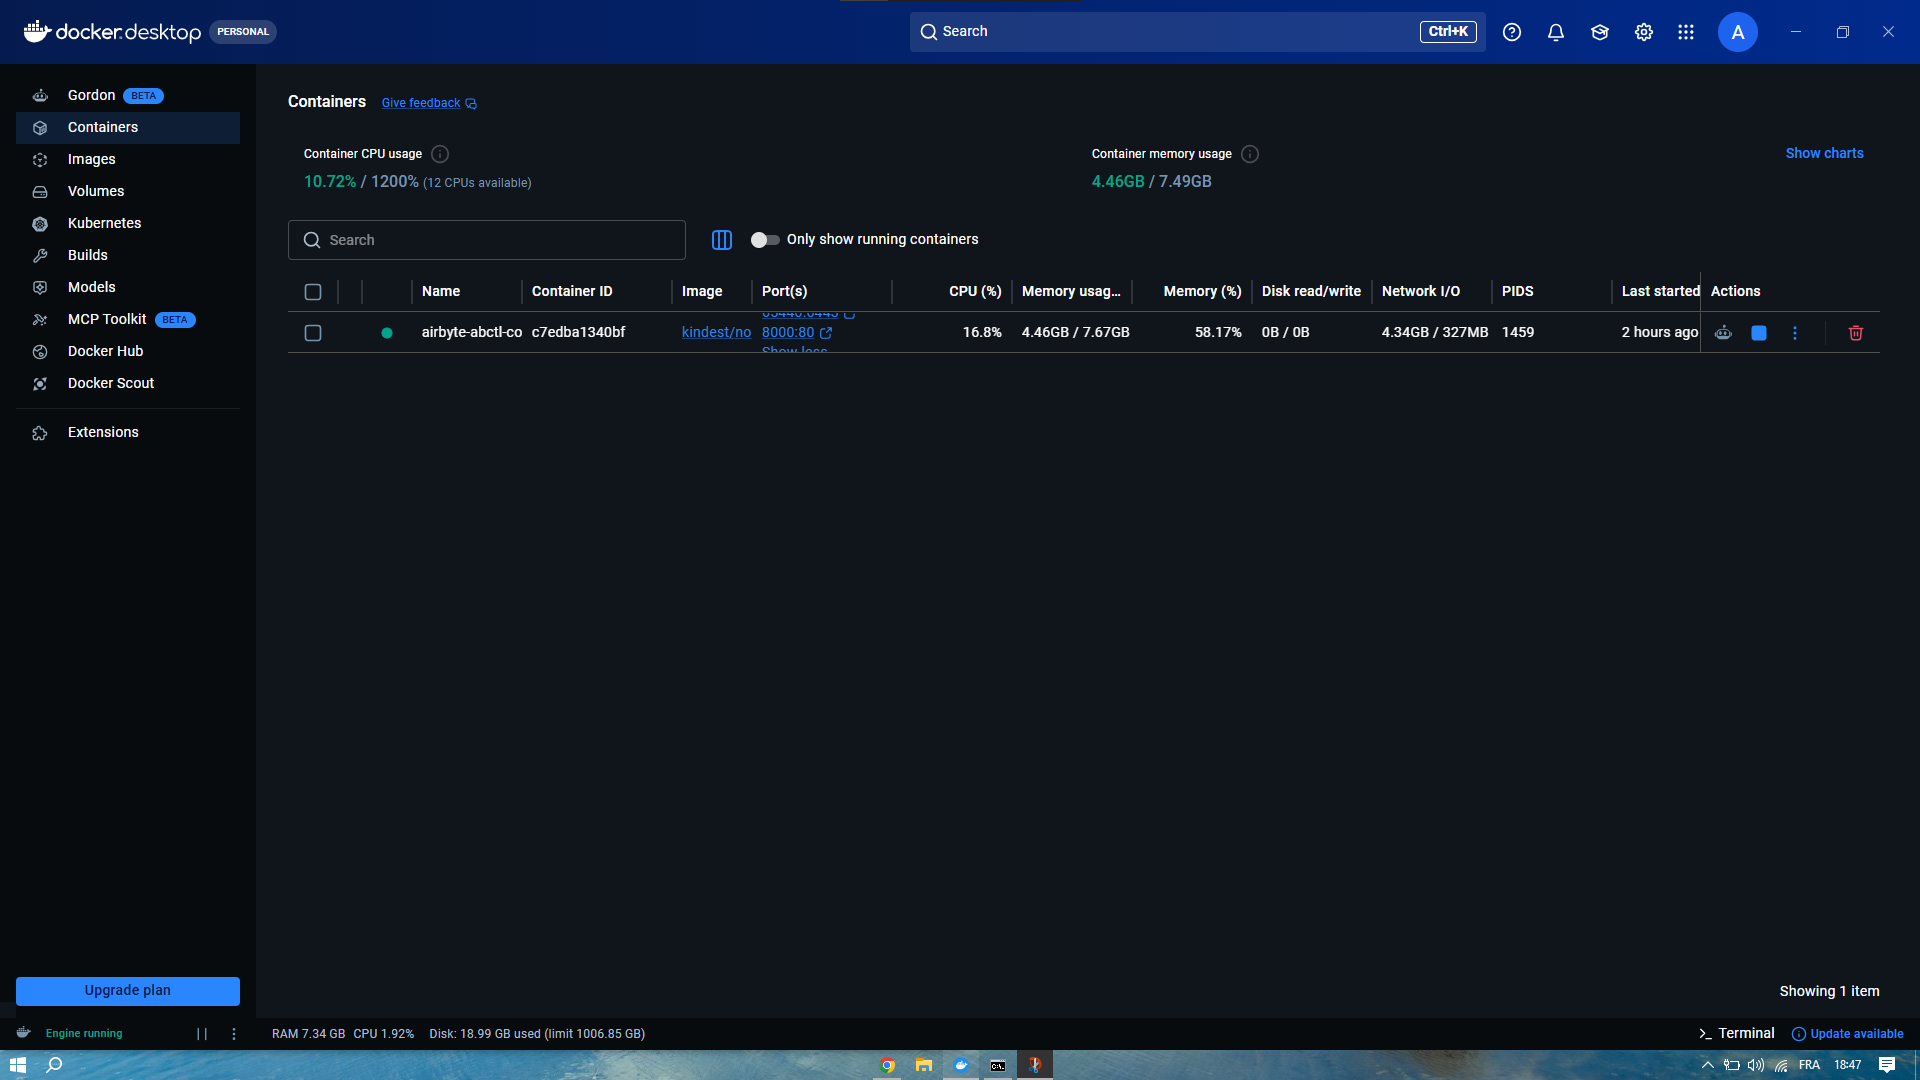
\includegraphics[width=0.85\textwidth]{figures/airbyte_docker_ui.png}
\caption{Airbyte UI home / workspace running in Docker}
\label{fig:airbyte_docker_ui}
\end{figure}
The Docker-hosted Airbyte workspace is the operational control plane from which all seven
CSV sources and the SQL Server destination are configured.

\begin{figure}[H]
\centering
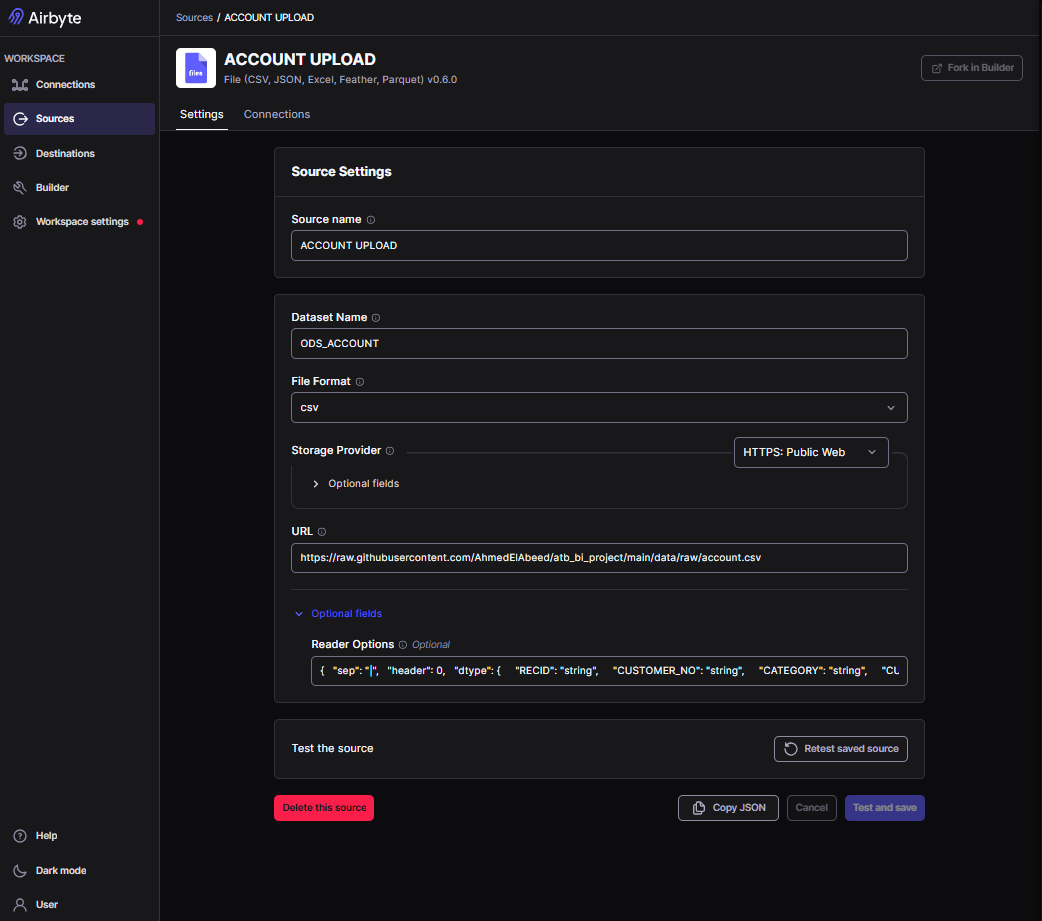
\includegraphics[width=0.7\textwidth]{figures/airbyte_github_source.png}
\caption{HTTPS source connector pointing to the GitHub raw CSV URL}
\label{fig:airbyte_github_source}
\end{figure}
Each source connector reads a pipe-delimited extract over HTTPS, avoiding fragile local
file paths on the developer workstation.

\begin{figure}[H]
\centering
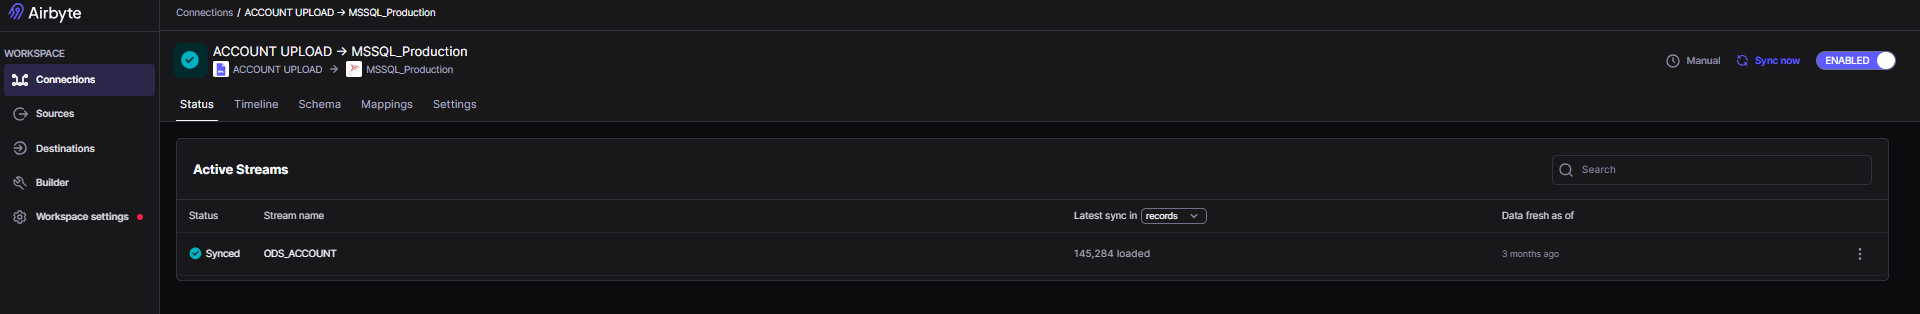
\includegraphics[width=0.85\textwidth]{figures/airbyte_connections_list.png}
\caption{List of the 7 Airbyte sync connections}
\label{fig:airbyte_connections_list}
\end{figure}
The connection list mirrors the seven raw datasets and makes sync status visible at a
glance before any dbt transformation runs.

\begin{figure}[H]
\centering
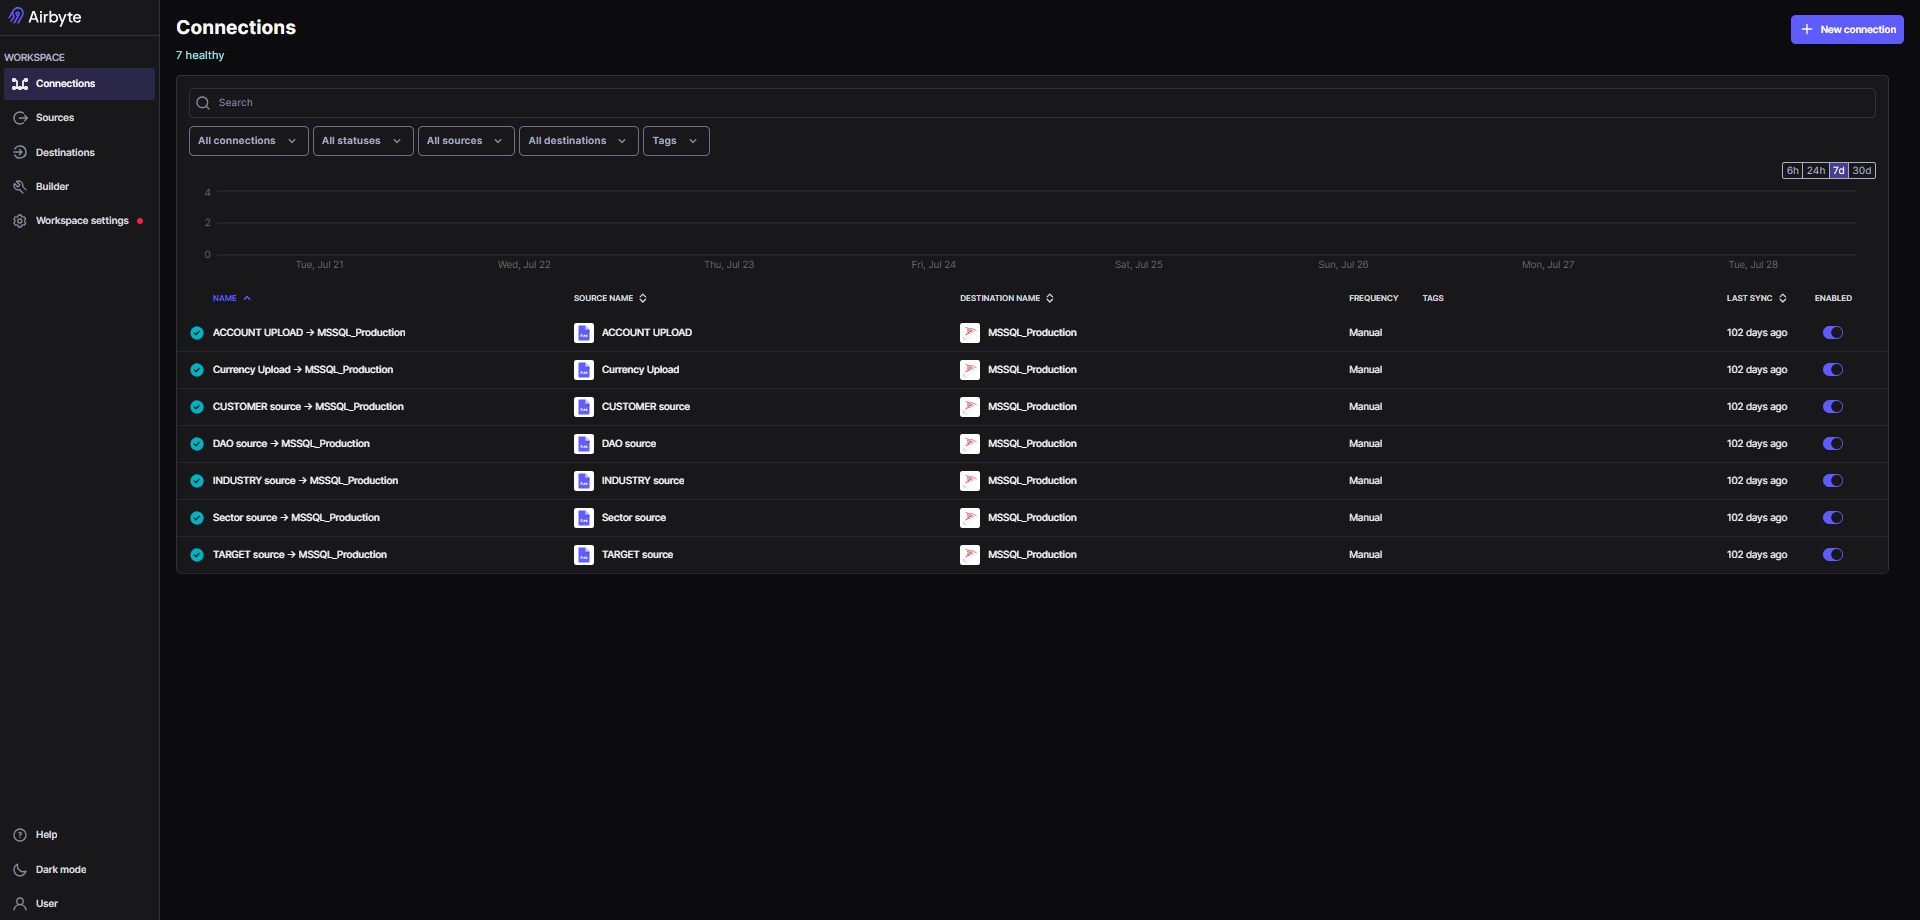
\includegraphics[width=0.85\textwidth]{figures/airbyte_sync_success.png}
\caption{Successful Airbyte sync job green status after loading into Database}
\label{fig:airbyte_sync_success}
\end{figure}
A green sync confirms that the ODS tables were refreshed and are ready for staging models.

\begin{figure}[H]
\centering
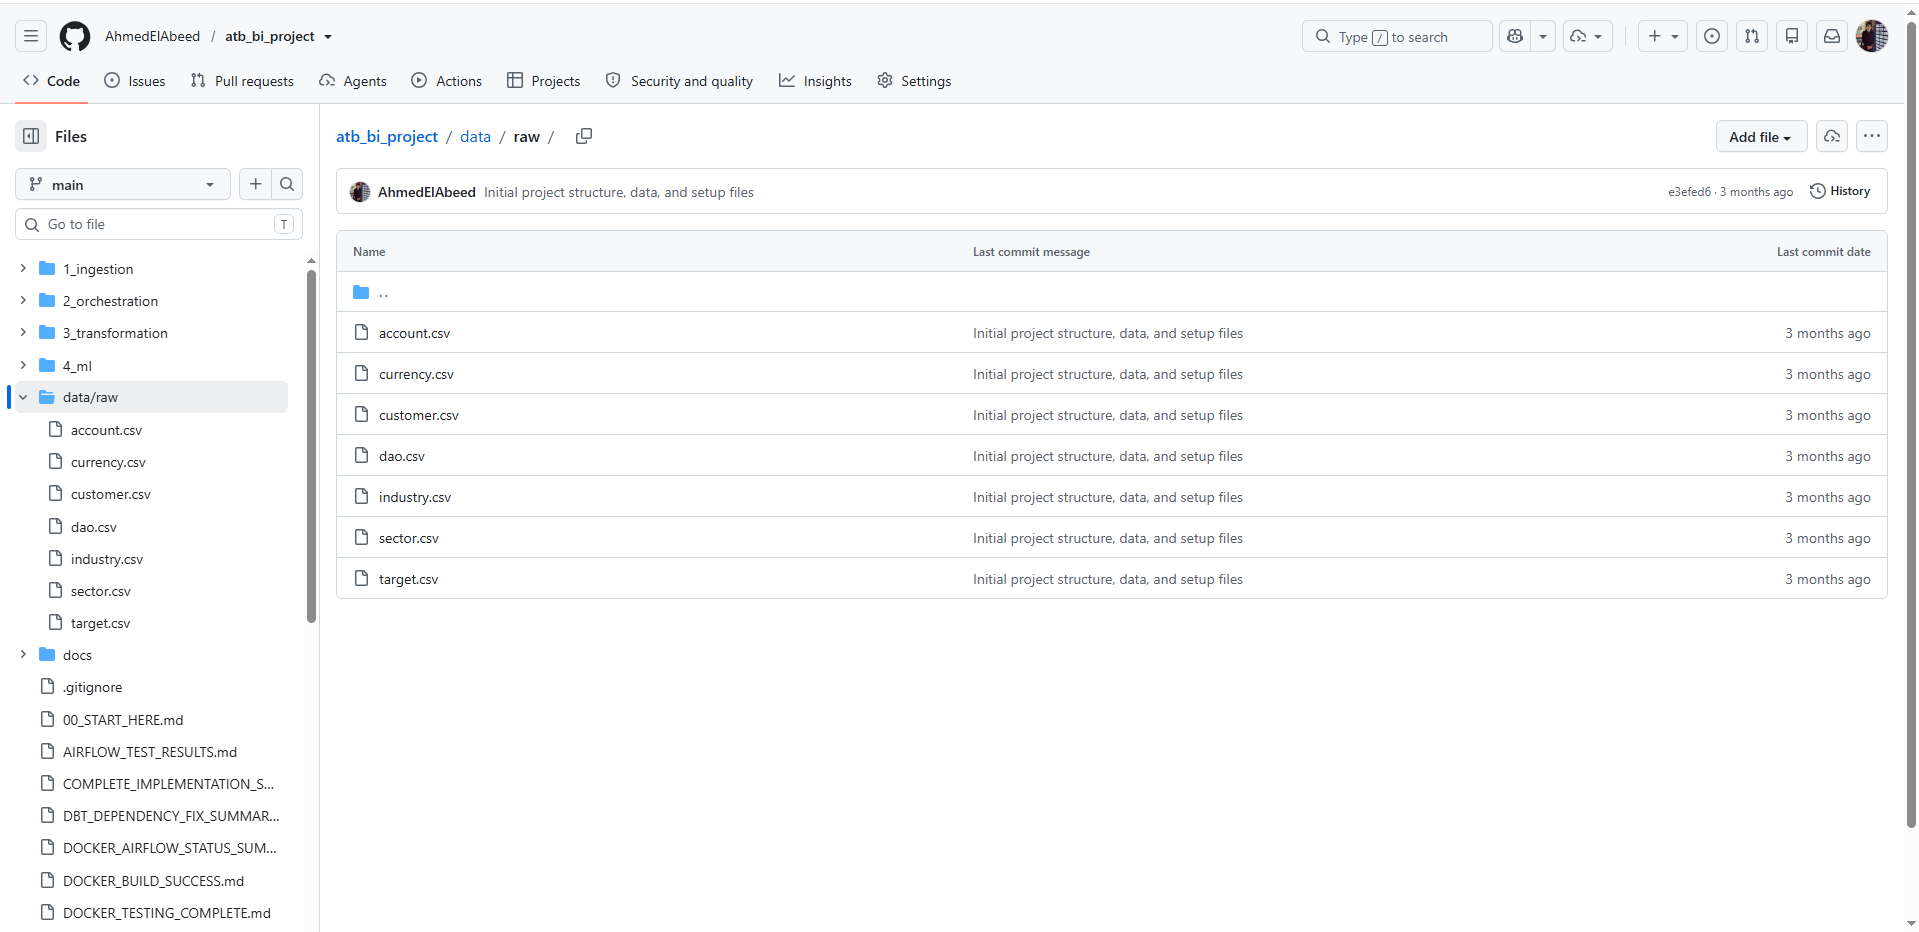
\includegraphics[width=0.85\textwidth]{figures/github_raw_csv.png}
\caption{GitHub repository view of raw CSV files in \texttt{data/raw/}}
\label{fig:github_raw_csv}
\end{figure}
Versioned extracts under \texttt{data/raw/} provide a single, auditable source location
for every Airbyte HTTPS connector.

\begin{figure}[H]
\centering
\begin{tikzpicture}[
  font=\scriptsize,
  box/.style={rectangle, rounded corners=2pt, draw=#1, fill=#1!10, thick,
              align=center, minimum width=2.45cm, minimum height=1.2cm},
  arr/.style={->, thick}
]
  \node[box=gray!70!black] (csv) {7 CSV files\\uploaded to GitHub};
  \node[box=orange!75!black, right=0.4cm of csv] (gh) {GitHub raw\\HTTPS URLs};
  \node[box=cyan!70!black, right=0.4cm of gh] (ab) {Airbyte\\(Docker)};
  \node[box=blue!70!black, right=0.4cm of ab] (ods) {\texttt{PFE\_ODS}\\SQL Server};
  \draw[arr] (csv) -- (gh);
  \draw[arr] (gh) -- (ab);
  \draw[arr] (ab) -- (ods);
\end{tikzpicture}
\caption{Source acquisition chain GitHub-hosted CSVs synchronised by Airbyte (Docker) into \texttt{ODS}}
\label{fig:airbyte_ingest_flow}
\end{figure}

\begin{figure}[H]
\centering
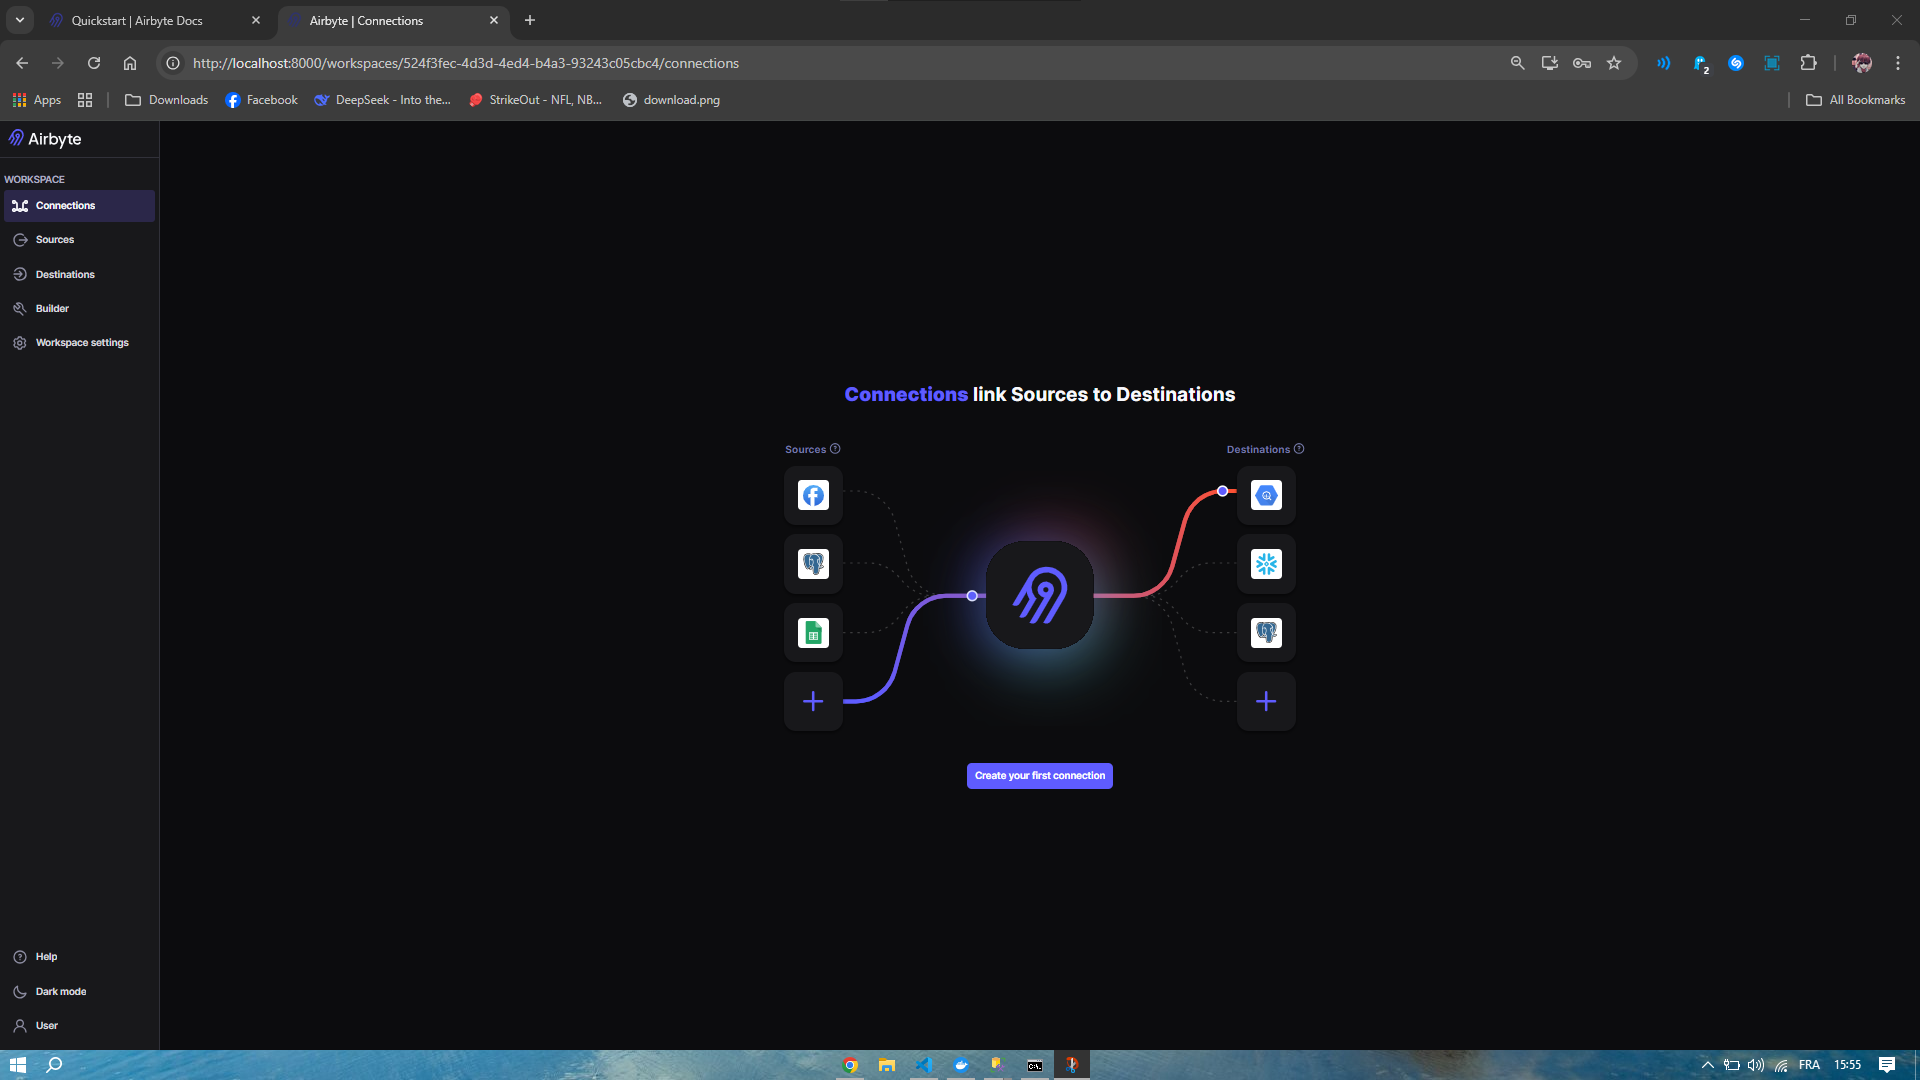
\includegraphics[width=0.55\textwidth]{figures/Airbyte_plateform.png}
\caption{Airbyte platform used as the ingestion engine of Release~2}
\label{fig:airbyte_logo_ref}
\end{figure}

Table~\ref{tab:raw_volumes} registers the measured volumes after a successful
sync. These counts later reappear almost one-to-one in the warehouse facts a
simple but reassuring integrity check.

\begin{table}[H]
\centering
\caption{Detailed volumetry of source datasets ingested by Airbyte}
\label{tab:raw_volumes}
\renewcommand{\arraystretch}{1.25}
\scriptsize
\begin{tabular}{|p{2.8cm}|c|c|p{7.0cm}|}
\hline
\rowcolor{blue!15}
\textbf{Source CSV} & \textbf{Rows} & \textbf{ODS table} & \textbf{Business content} \\
\hline
\texttt{customer.csv} & $136{,}676$ & \texttt{ODS\_CUSTOMER} & Identity, employment, salary, KYC/PEP/compliance flags, DAO link. \\
\hline
\texttt{account.csv} & $145{,}284$ & \texttt{ODS\_ACCOUNT} & Working balances, opening dates, currency, officer link. \\
\hline
\texttt{dao.csv} & $150$ & \texttt{ODS\_DAO} & Desk Account Officers, branch areas and names. \\
\hline
\texttt{currency.csv} & $22$ & \texttt{ODS\_CURRENCY} & ISO currency reference. \\
\hline
\texttt{sector.csv} & $45$ & \texttt{ODS\_SECTOR} & Macro-economic sectors. \\
\hline
\texttt{industry.csv} & $663$ & \texttt{ODS\_INDUSTRY} & Detailed activity codes. \\
\hline
\texttt{target.csv} & $11$ & \texttt{ODS\_TARGET} & Client segments (retail, SME, corporate,\ldots). \\
\hline
\end{tabular}
\end{table}

In plain words: GitHub stores the files, Docker runs Airbyte, SQL Server receives
the ODS tables, and Airflow later triggers the same syncs every night. That is
the ingestion backbone behind US~04.

%======================================================================
\section{Phase 2: Design}
\label{sec:gimsi_phase2}
%======================================================================
The second GIMSI phase translates decision-maker needs into measurable indicators
and designs the data model that will compute them.

\subsection{Design Methodology: Kimball Approach and Dimensional Modelling}
The physical modelling of the decision warehouse relies rigorously on the
dimensional modelling concepts theorised by Ralph Kimball \cite{kimball2013}.
This approach pursues two essential objectives in decision engineering:
facilitate intuitive data exploration for business users, and optimise analytical
query performance by limiting join complexity.

\paragraph{Conformed dimensions and surrogate keys.}
The constellation structure rests on sharing \textbf{conformed dimensions}
across business processes. These dimensions constitute the unique, standardised
referential of the warehouse:
\begin{itemize}
    \item \texttt{dim\_customer} --- demographics, tenure, KYC/PEP/compliance attributes;
    \item \texttt{dim\_dao} --- account officer and branch/area mapping;
    \item \texttt{dim\_date} --- calendar attributes for openings and scoring dates;
    \item \texttt{dim\_sector}, \texttt{dim\_industry}, \texttt{dim\_target} ---
          economic and commercial segmentation;
    \item \texttt{dim\_currency} --- ISO codes plus an \texttt{UNK} sentinel;
    \item \texttt{dim\_risk\_profile} --- historical three-pillar scores per scoring date.
\end{itemize}

Referential integrity is guaranteed by \textbf{surrogate keys} (e.g.\
\texttt{customer\_sk}, \texttt{dao\_sk}). Each dimension holds a system-generated
integer identifier independent of volatile source business keys. This isolates
the warehouse from upstream key changes and accelerates SQL joins required by
visual restitutions.

\paragraph{Fact tables and constellation (galaxy) structure.}
The ATB constellation materialises through two complementary fact tables connected
to the conformed dimensions:
\begin{itemize}
    \item \texttt{fact\_account} --- transactional balance snapshot (grain: one row
          per account);
    \item \texttt{fact\_customer\_risk} --- scored risk profile (grain: one row per
          customer per scoring date).
\end{itemize}
Crossing both facts via shared dimensions (customer, DAO, sector,\ldots) enables
advanced analyses such as: \emph{average risk of overdrawn accounts in the Tunis
Centre area, by industry}.

\paragraph{Bottom-up architecture and agile integration.}
Contrary to Bill Inmon's top-down 3NF enterprise warehouse --- complex to deploy
up-front --- we adopted Kimball's \textbf{bottom-up} architecture:
\begin{itemize}
    \item \textbf{Incremental agile delivery:} Release~1 prepared orchestration and
          security; Release~2 grafts the constellation and dashboard without
          destabilising the foundation, matching the Scrum sprint cadence.
    \item \textbf{Performance through controlled denormalisation:} limiting join
          depth is essential for fast Plotly rendering on Streamlit.
\end{itemize}

\subsection{Dimensional Modelling: Constellation Schema}
Figure~\ref{fig:galaxy_schema_ref} shows the production constellation diagram;
Figure~\ref{fig:constellation_tikz} abstracts the same model as a TikZ schematic
for academic clarity.

\begin{figure}[H]
\centering
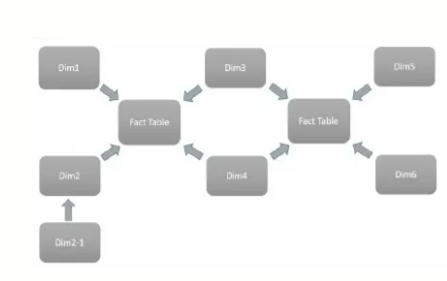
\includegraphics[width=0.82\textwidth]{figures/galaxy_schema.png}
\caption{ATB Kimball constellation schema  conformed dimensions shared by
Both fact tables}
\label{fig:galaxy_schema_ref}
\end{figure}

\begin{figure}[H]
\centering
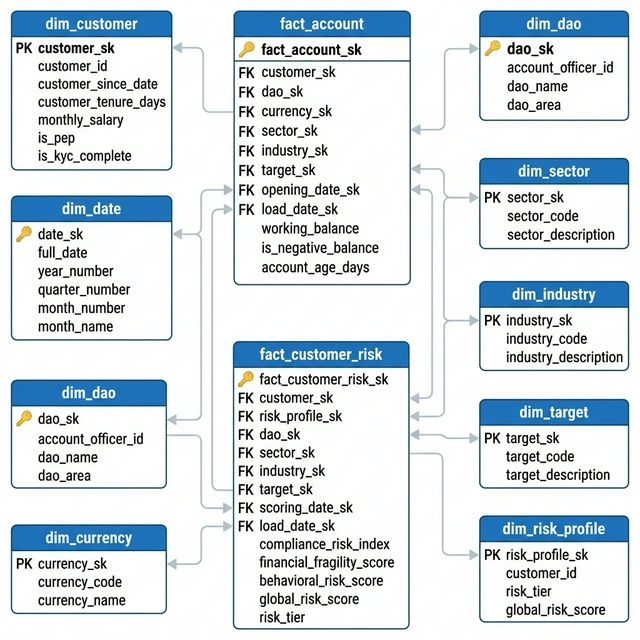
\includegraphics[width=0.85\textwidth]{figures/constellation view model.png}
\caption{Abstract constellation view shared conformed dimensions around two facts}
\label{fig:constellation_tikz}
\end{figure}

\paragraph{Reuse of engineered features in the BI dashboard.}
Variables produced in the intermediate dbt layer (pillar scores, account
aggregates, tenure, overdraft flags) are not reserved for Machine Learning. They
constitute the \textbf{computational substrate of the BI dashboard}. The business
layer reads the same warehouse measures that will later feed Release~3 models,
avoiding redundant calculation and guaranteeing consistency between descriptive
KPIs and future predictive scores.
\subsection{Fact Modelling, Table Content and KPI Justification}
\begin{itemize}
    \item \textbf{Central fact \texttt{fact\_customer\_risk}} ($136{,}676$ rows):
          foreign keys to customer, DAO, sector, industry, target, risk profile and
          date; measures CRI, FFS, BRS, GRS, \texttt{risk\_tier}, account counts and
          balances.
    \item \textbf{Operational fact \texttt{fact\_account}} ($145{,}284$ rows):
          foreign keys to customer, DAO, currency, sector, industry, target and
          opening/load dates; measures \texttt{working\_balance},
          \texttt{is\_negative\_balance}, \texttt{account\_age\_days}.
\end{itemize}

\paragraph{Strategic justification of KPIs.}
Each indicator answers a precise managerial objective. KPIs are grouped by their
fact of origin.

\begin{table}[H]
\centering
\caption{Decision and technical justification of KPIs from \texttt{fact\_account}}
\label{tab:kpi_fact_account}
\renewcommand{\arraystretch}{1.2}
\scriptsize
\begin{tabular}{|p{3.5cm}|p{5.0cm}|p{6.0cm}|}
\hline
\rowcolor{blue!25}
\textbf{KPI} & \textbf{Technical definition} & \textbf{Business rationale} \\
\hline
Total balance exposure & $\sum \texttt{working\_balance}$ & Monitors funds held / overdrawn at bank level. \\
\hline
Overdraft rate & $\dfrac{|\{a: b_a<0\}|}{|A|}\times 100\%$ & Immediate solvency pressure signal. \\
\hline
Average account age & $\mathrm{mean}(\texttt{account\_age\_days})$ & Maturity of the customer relationship. \\
\hline
\end{tabular}
\end{table}

\begin{table}[H]
\centering
\caption{Decision and technical justification of KPIs from \texttt{fact\_customer\_risk}}
\label{tab:kpi_fact_risk}
\renewcommand{\arraystretch}{1.2}
\scriptsize
\begin{tabular}{|p{3.5cm}|p{5.0cm}|p{6.0cm}|}
\hline
\rowcolor{blue!25}
\textbf{KPI} & \textbf{Technical definition} & \textbf{Business rationale} \\
\hline
Average Global Risk Score & $\mathrm{mean}(\mathrm{GRS})$ & Single health index of the portfolio. \\
\hline
High-risk ratio & Share with $\mathrm{GRS}\ge 50$ & Population requiring closer follow-up. \\
\hline
Pillar averages & $\mathrm{mean}(\mathrm{CRI})$, $\mathrm{mean}(\mathrm{FFS})$, $\mathrm{mean}(\mathrm{BRS})$ & Explains \emph{why} risk is elevated. \\
\hline
KYC completion rate & Share with \texttt{is\_kyc\_complete}=1 & Regulatory readiness thermometer. \\
\hline
Risk-tier mix & Counts by \texttt{LOW}/\texttt{MEDIUM}/\texttt{HIGH}/\texttt{VERY\_HIGH} & Distributional view for committees. \\
\hline
\end{tabular}
\end{table}

\subsection{Creation of KPIs and Visual Dashboards}
From the requirements model, we defined a set of KPIs and analytical
visualisations that structure managerial steering. Technically, aggregations are
executed in SQL/Pandas while \textbf{Plotly} renders interactive vector graphics
inside Streamlit. Restitutions are categorised into two complementary levels.

\subsubsection*{1. Numeric indicators (metric cards)}
Placed in the page header, these indicators provide an immediate quantitative
synthesis of the analysed portfolio. They are grouped into four thematic
clusters: \textbf{Portfolio}, \textbf{Risk}, \textbf{Compliance} and
\textbf{Financial / Behavioural}. Each card is re-computed at every Airflow
nightly run so that the value displayed always reflects the latest warehouse
snapshot.

\begin{table}[H]
\centering
\caption{Comprehensive specifications of numeric dashboard KPI indicators}
\label{tab:kpis_chiffres}
\renewcommand{\arraystretch}{1.22}
\scriptsize
\begin{tabular}{|p{0.6cm}|p{3.0cm}|p{5.1cm}|p{5.6cm}|}
\hline
\rowcolor{blue!15}
\textbf{\#} & \textbf{KPI} & \textbf{Algorithmic translation} & \textbf{Analytical objective} \\
\hline
\multicolumn{4}{|l|}{\cellcolor{blue!8}\textit{\textbf{A --- Portfolio overview}}} \\
\hline
A1 & Total customers & \texttt{COUNT(DISTINCT customer\_sk)} on \texttt{fact\_customer\_risk} & Portfolio volumetry; baseline denominator for all rate KPIs. \\
\hline
A2 & Total accounts & \texttt{COUNT(*)} on \texttt{fact\_account} & Measures product penetration; ratio with A1 gives accounts-per-customer. \\
\hline
A3 & Accounts per customer & $\dfrac{\text{A2}}{\text{A1}}$ & Relationship depth indicator; single-account profiles flag fragility. \\
\hline
A4 & Total balance exposure & \texttt{SUM(working\_balance)} on \texttt{fact\_account} & Net cash position of the entire book; negative total signals systemic overdraft stress. \\
\hline
A5 & Average account age (days) & \texttt{AVG(account\_age\_days)} & Relationship maturity; older books are generally more stable. \\
\hline
\multicolumn{4}{|l|}{\cellcolor{blue!8}\textit{\textbf{B --- Risk scoring}}} \\
\hline
B1 & Average Global Risk Score & \texttt{AVG(global\_risk\_score)} on \texttt{fact\_customer\_risk} & Single health index of the portfolio; values near 25--50 indicate a retail distribution. \\
\hline
B2 & High-risk customer \% & $\dfrac{|\{c:\mathrm{GRS}\ge 50\}|}{\text{A1}}\times 100\%$ & Mass of customers requiring credit or compliance escalation. \\
\hline
B3 & Very-high-risk \% & $\dfrac{|\{c:\mathrm{GRS}\ge 75\}|}{\text{A1}}\times 100\%$ & Tier~4 customers: immediate managerial intervention required. \\
\hline
B4 & Average CRI & \texttt{AVG(cri\_score)} & Compliance risk pressure across the book; spikes signal KYC/PEP deterioration. \\
\hline
B5 & Average FFS & \texttt{AVG(ffs\_score)} & Financial fragility pressure; tracks salary and overdraft stress. \\
\hline
B6 & Average BRS & \texttt{AVG(brs\_score)} & Behavioural early-warning index; correlates with tenure and thin balances. \\
\hline
\multicolumn{4}{|l|}{\cellcolor{blue!8}\textit{\textbf{C --- Compliance and regulatory}}} \\
\hline
C1 & KYC completion rate & $\dfrac{|\{c:\texttt{is\_kyc\_complete}=1\}|}{\text{A1}}\times 100\%$ & Regulatory readiness; below 95\% triggers watchlist escalation. \\
\hline
C2 & PEP exposure \% & $\dfrac{|\{c:\texttt{is\_pep}=1\}|}{\text{A1}}\times 100\%$ & Politically exposed persons share; key FATF monitoring obligation. \\
\hline
C3 & Compliance-flagged \% & $\dfrac{|\{c:\texttt{is\_compliance\_flagged}=1\}|}{\text{A1}}\times 100\%$ & Active compliance files requiring CCO review. \\
\hline
C4 & Stale KYC review \% & Share with last KYC date $>365$ days & Periodic review backlog; regulatory SLA breach indicator. \\
\hline
\multicolumn{4}{|l|}{\cellcolor{blue!8}\textit{\textbf{D --- Financial and solvency}}} \\
\hline
D1 & Overdraft customer \% & $\dfrac{|\{c:\text{total balance}<0\}|}{\text{A1}}\times 100\%$ & Solvency alert rate; drives credit follow-up queue. \\
\hline
D2 & Near-zero balance \% & Share with $\texttt{working\_balance}\in[0,500]$ & Latent fragility; customers one shock away from overdraft. \\
\hline
D3 & Unemployed customer \% & Share with employment \texttt{UNEMPLOYED} / \texttt{CHOMEUR} & Social risk dimension; correlates with FFS spikes. \\
\hline
\end{tabular}
\end{table}

\subsubsection*{2. Graphical visualisations (data visualisation)}
Interactive charts allow multi-dimensional correlation exploration.

\begin{table}[H]
\centering
\caption{Specifications of decision visualisations}
\label{tab:kpis_graphiques}
\renewcommand{\arraystretch}{1.25}
\scriptsize
\begin{tabular}{|p{3.2cm}|p{3.6cm}|p{7.0cm}|}
\hline
\rowcolor{blue!15}
\textbf{Chart component} & \textbf{Implementation} & \textbf{Visual analysis objective} \\
\hline
Risk-tier mix & Pie / donut (\texttt{px.pie}) & Portfolio composition by risk class. \\
\hline
Sector / industry bars & Bar chart (\texttt{px.bar}) & Concentration of balances or risk. \\
\hline
Sector $\times$ area heatmap & Heatmap & Hot spots for regional follow-up. \\
\hline
Salary vs.\ risk & Scatter (\texttt{px.scatter}) & Financial fragility patterns. \\
\hline
KYC / PEP breakdowns & Grouped bars & Compliance workload. \\
\hline
Tenure bands & Bar / box & Behavioural maturity effects. \\
\hline
\end{tabular}
\end{table}

Colour coding is consistent across the application:
\texttt{LOW}, \texttt{MEDIUM},
\texttt{HIGH}, \texttt{VERY\_HIGH}.

%======================================================================
\section{Phase 3: Realisation}
\label{sec:gimsi_phase3}
%======================================================================
The realisation phase is the operational heart of decision engineering. It
physically implements the BI architecture through four fundamental layers:
Access (ELT), Warehouse, Business and Presentation.

Deliverables of this phase are: a modular and reproducible dbt ELT pipeline, a
constellation warehouse optimised for analytical queries, a set of engineered
risk features and pillar scores, and a Streamlit presentation layer with RBAC.

\subsection{Layer 1: Data Access}
This first layer executes the three ELT phases (\textit{Extract},
\textit{Load}, \textit{Transform}), orchestrated by Airflow and implemented as
versioned SQL models under dbt.

Figure~\ref{fig:elt_four_layers} situates Layer~1 inside the global four-layer
stack.

\begin{figure}[H]
\centering
\begin{tikzpicture}[
  font=\small,
  layer/.style={rectangle, rounded corners=3pt, draw=#1, fill=#1!12, thick,
                align=center, minimum width=12.2cm, minimum height=1.05cm},
  arr/.style={->, thick, gray!60}
]
  \node[layer=cyan!70!black] (l1) {\textbf{Layer 1 --- Access:} Airbyte $\rightarrow$ \texttt{PFE\_ODS} $\rightarrow$ dbt staging / intermediate};
  \node[layer=blue!70!black, below=0.35cm of l1] (l2) {\textbf{Layer 2 --- Warehouse:} 8 dimensions + 2 facts in \texttt{PFE\_DWH}};
  \node[layer=violet!70!black, below=0.35cm of l2] (l3) {\textbf{Layer 3 --- Business:} SQL/Pandas KPI aggregations + RBAC filters};
  \node[layer=orange!80!black, below=0.35cm of l3] (l4) {\textbf{Layer 4 --- Presentation:} Streamlit pages, Plotly, Gemini explanations, export};
  \draw[arr] (l1) -- (l2);
  \draw[arr] (l2) -- (l3);
  \draw[arr] (l3) -- (l4);
\end{tikzpicture}
\caption{Four-layer BI architecture realised in Sprint~3}
\label{fig:elt_four_layers}
\end{figure}

\paragraph{Extract / Load phase --- Airbyte into \texttt{PFE\_ODS}.}
As described in Phase~1, GitHub-hosted CSVs are pulled by Airbyte Docker
connectors into \texttt{ODS\_*} tables. Before analytical use we enforce three
simple contracts:
\begin{itemize}
    \item \textbf{Delimiter:} pipe (\texttt{|}) so commas inside text fields stay safe;
    \item \textbf{Encoding:} UTF-8 for Tunisian/French labels;
    \item \textbf{Primary-key integrity:} uniqueness checks on customer and account
          identifiers in staging tests.
\end{itemize}
This isolates \emph{collection} (Airbyte) from \emph{cleaning} (dbt).

\paragraph{Transform phase --- Staging: nulls, types and bilingual flags.}
\label{sec:staging_cleaning}
Raw banking extracts are rarely analysis-ready. Empty strings, mixed French/English
booleans, malformed dates and duplicate keys are normal. The staging models
(\texttt{stg\_customer}, \texttt{stg\_account}, \texttt{stg\_dao},
\texttt{stg\_sector}, \texttt{stg\_industry}, \texttt{stg\_currency},
\texttt{stg\_target}) are where we make the data \emph{boring in a good way}:
predictable types, one meaning per flag, no silent blanks.

\textbf{1.\ Null and blank handling.}
Operational files often store missing values as empty text (\texttt{''}) instead
of SQL \texttt{NULL}. Staging systematically applies
\texttt{nullif(ltrim(rtrim(...)), '')} so blanks become true nulls, then:
\begin{itemize}
    \item numeric fields use \texttt{try\_cast} / \texttt{try\_convert} (invalid
          tokens become NULL instead of crashing the run);
    \item codes fall back with \texttt{coalesce(..., 'UNKNOWN')} when a default is
          safer for joins;
    \item dependents default to $0$ when missing; turnover defaults to $0.00$;
    \item unparseable opening/customer-since dates fall back to
          \texttt{1900-01-01} and raise a parse-quality flag for audit.
\end{itemize}

\textbf{2.\ Bilingual Yes/No standardisation (\texttt{OUI}/\texttt{NON}/\texttt{YES}/\texttt{NO}).}
ATB source fields mix French and English boolean vocabularies
(\texttt{KYC\_COMPLETE}, \texttt{L\_PEP}, \texttt{L\_FLAG\_CONF},
\texttt{L\_DECS\_CONF}). Leaving them as free text would break every KPI that
counts ``true'' customers. In \texttt{stg\_customer} we therefore map them to
strict SQL bits:
\begin{equation}
\texttt{is\_*} =
\begin{cases}
1 & \text{if }\mathrm{upper}(v)\in\{\texttt{OUI},\texttt{YES},\texttt{Y},\texttt{1},\texttt{TRUE}\}\\
0 & \text{if }\mathrm{upper}(v)\in\{\texttt{NON},\texttt{NO},\texttt{N},\texttt{0},\texttt{FALSE}\}\\
0 & \text{otherwise (including NULL / unknown)}
\end{cases}
\end{equation}
The same rule is applied to:
\begin{itemize}
    \item \texttt{is\_kyc\_complete} $\leftarrow$ \texttt{KYC\_COMPLETE};
    \item \texttt{is\_pep} $\leftarrow$ \texttt{L\_PEP};
    \item \texttt{is\_compliance\_flagged} $\leftarrow$ \texttt{L\_FLAG\_CONF};
    \item \texttt{has\_compliance\_decision} $\leftarrow$ \texttt{L\_DECS\_CONF}.
\end{itemize}
After this step, dashboard filters and risk points can test a single bit instead
of guessing language.

\textbf{3.\ Text and code standardisation.}
Nationality, residence, gender, marital status, employment status and currency
codes are trimmed and uppercased. Currency missing values are normalised toward
a controlled code list (with \texttt{UNK} reserved for the warehouse sentinel).

\textbf{4.\ Deduplication and orphan audits.}
Window functions (\texttt{row\_number} partitioned by natural keys) keep one
canonical row per customer/account/code. Dedicated audit models
(\texttt{audit\_invalid\_customer\_industry},
\texttt{audit\_invalid\_customer\_target}) list codes that do not resolve to
reference tables --- useful for data stewards, not for silent joins.

\begin{table}[H]
\centering
\caption{Staging cleaning rules applied before warehouse load}
\label{tab:staging_cleaning_rules}
\renewcommand{\arraystretch}{1.2}
\scriptsize
\begin{tabular}{|p{3.4cm}|p{5.2cm}|p{5.6cm}|}
\hline
\rowcolor{blue!15}
\textbf{Problem in raw CSV} & \textbf{Staging treatment} & \textbf{Why it matters} \\
\hline
Empty string instead of NULL & \texttt{nullif(trim(col),'')} & True missingness for KPIs and joins \\
\hline
\texttt{OUI}/\texttt{NON}/\texttt{YES}/\texttt{NO} & Map to bit $1/0$ & Language-proof compliance counts \\
\hline
Dirty dates (\texttt{YYYYMMDD} text) & \texttt{try\_convert(...,112)} & Tenure and KYC age become computable \\
\hline
Duplicate natural keys & \texttt{row\_number}=1 keep & Grain of facts stays unique \\
\hline
Unknown currency / category & \texttt{coalesce} + later sentinel $-1$ & Zero NULL foreign keys in facts \\
\hline
Orphan industry/target codes & Audit models (warn) & Data-quality backlog for ATB \\
\hline
\end{tabular}
\end{table}

\begin{figure}[H]
\centering
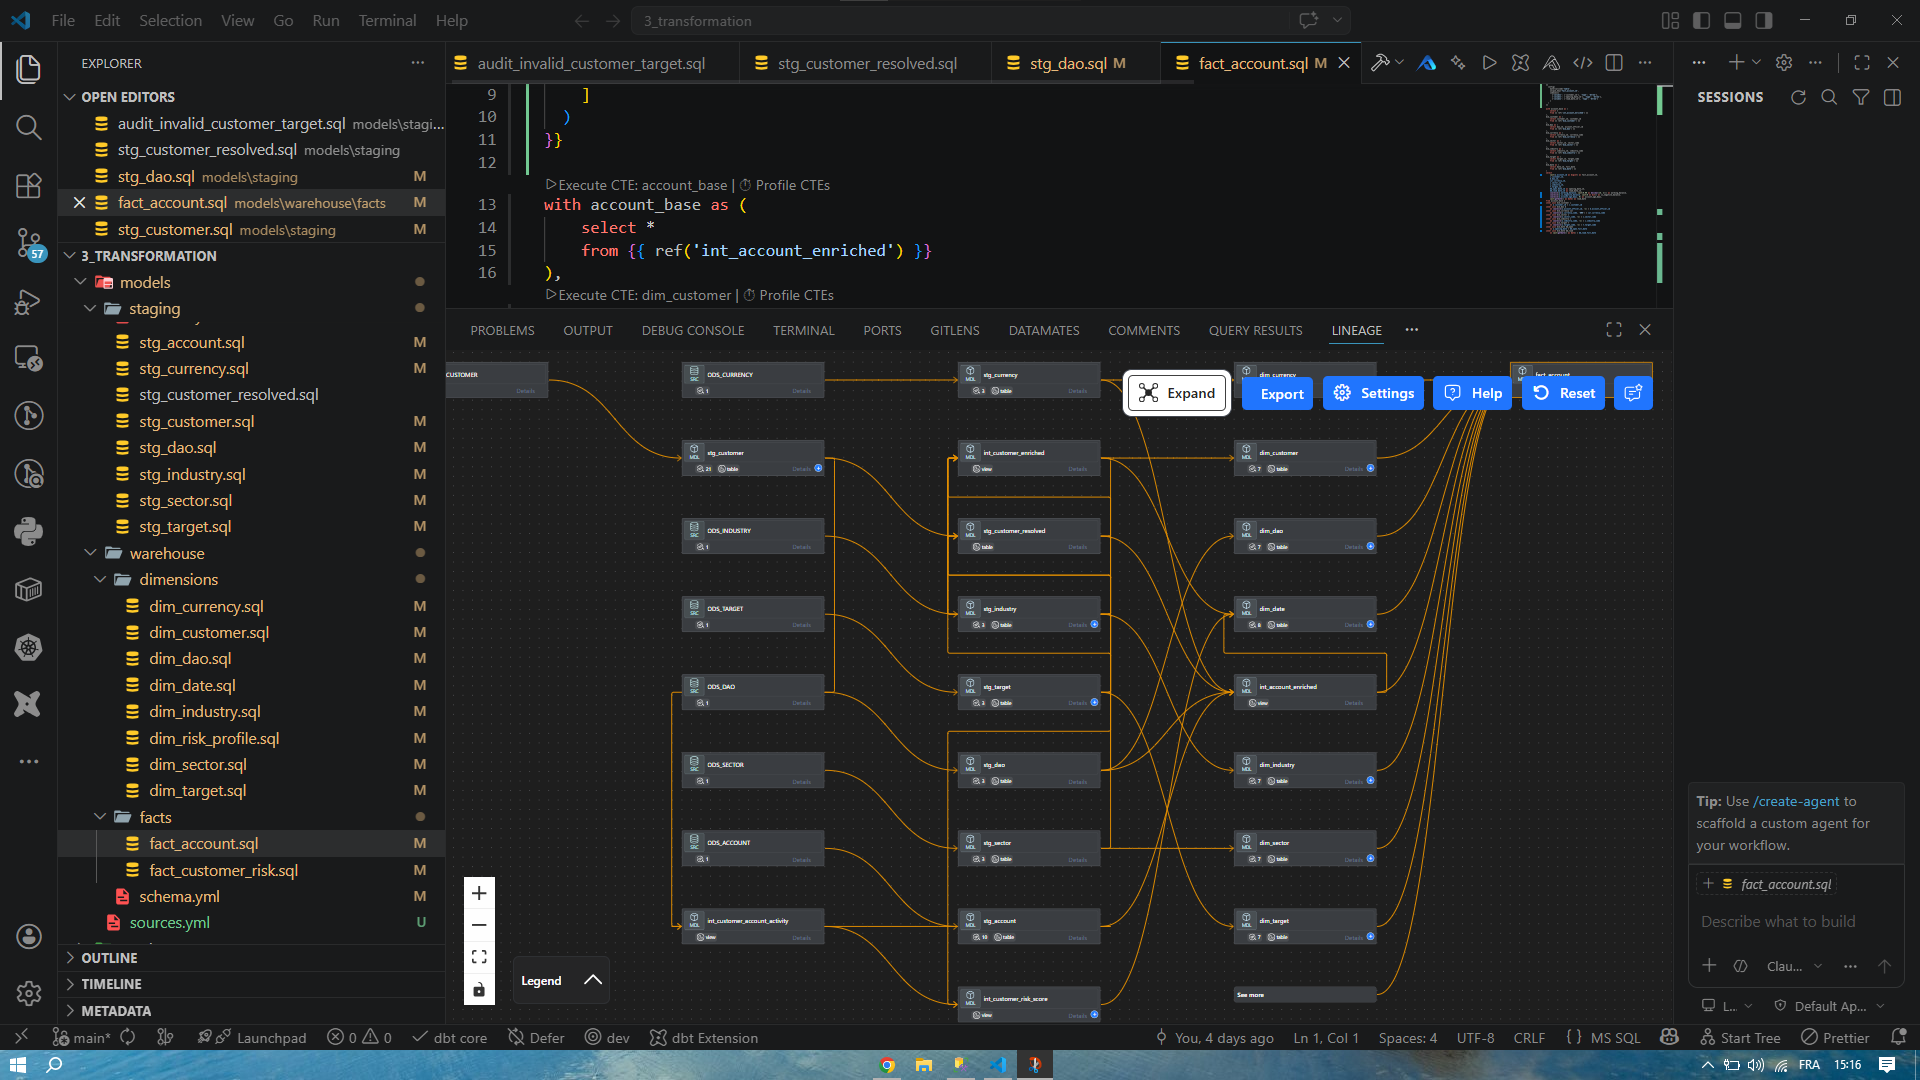
\includegraphics[width=0.85\textwidth]{figures/dbt_stg_customer_sql.png}
\caption{Excerpt of \texttt{stg\_customer.sql} showing the \texttt{OUI}/\texttt{NON} \texttt{CASE} mapping}
\label{fig:stg_customer_sql}
\end{figure}
Staging models translate French source flags into typed Boolean columns that downstream
risk SQL can reuse without ad hoc string parsing.

\begin{figure}[H]
\centering
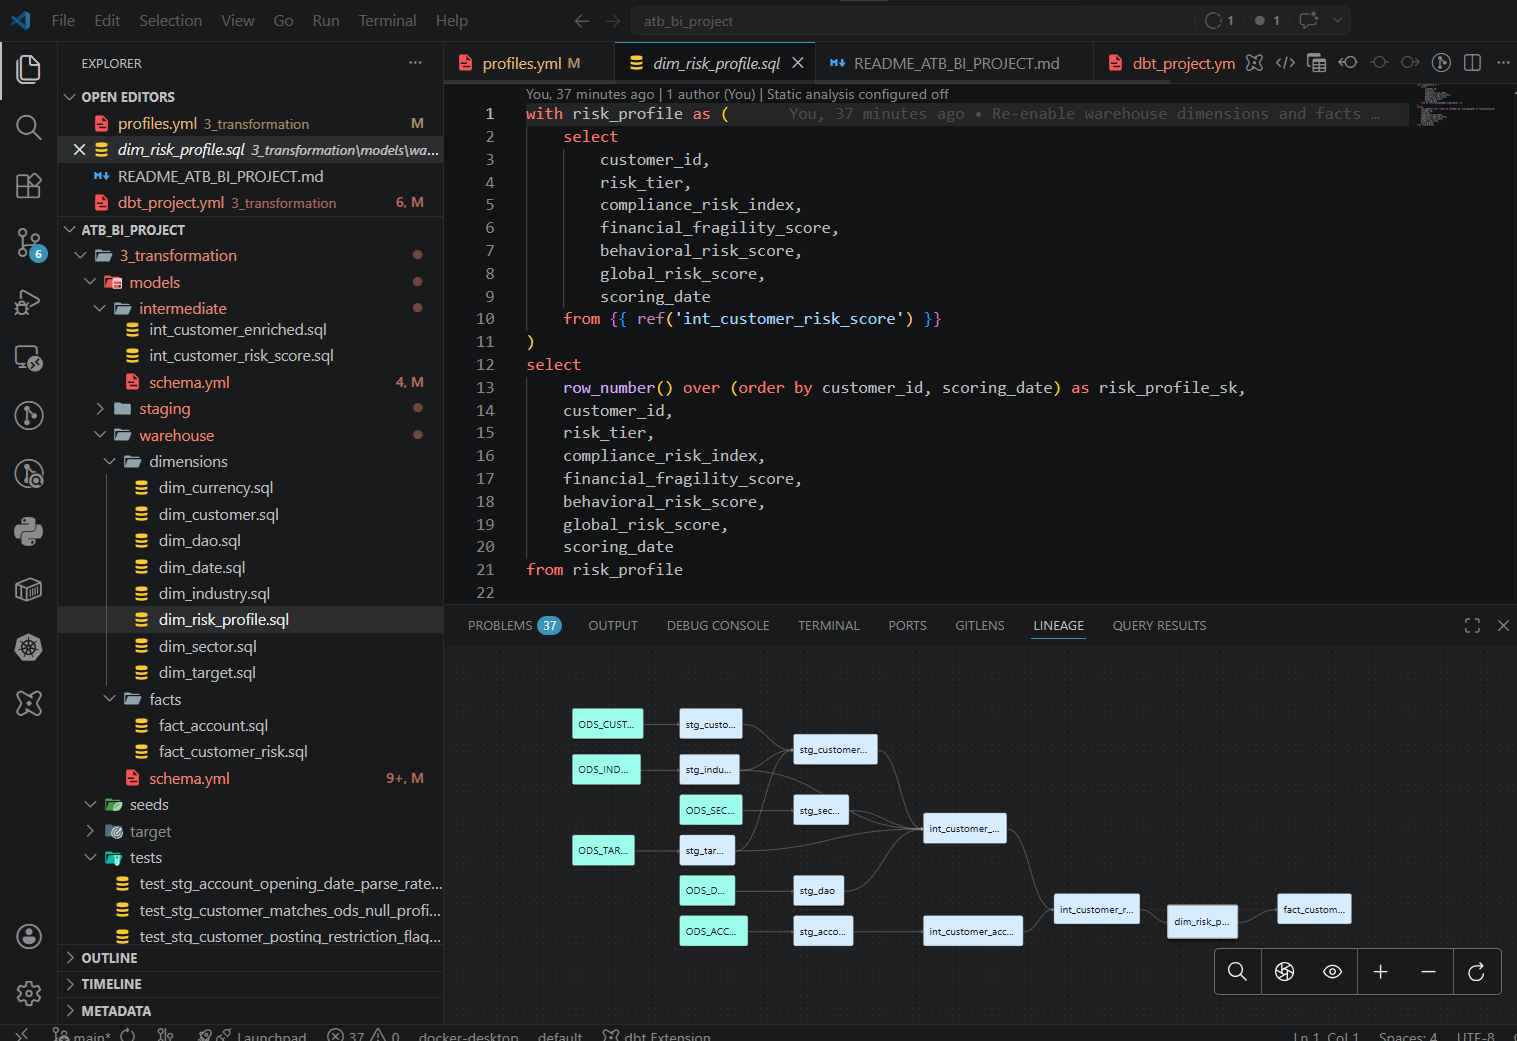
\includegraphics[width=0.85\textwidth]{figures/dbt_test_pass.png}
\caption{dbt test results --- \texttt{not\_null} / \texttt{unique} / \texttt{relationships} all green}
\label{fig:dbt_test_pass}
\end{figure}
Green \texttt{not\_null}, \texttt{unique} and \texttt{relationships} tests form the first
automated quality gate before intermediate risk models are built.

\begin{figure}[H]
\centering
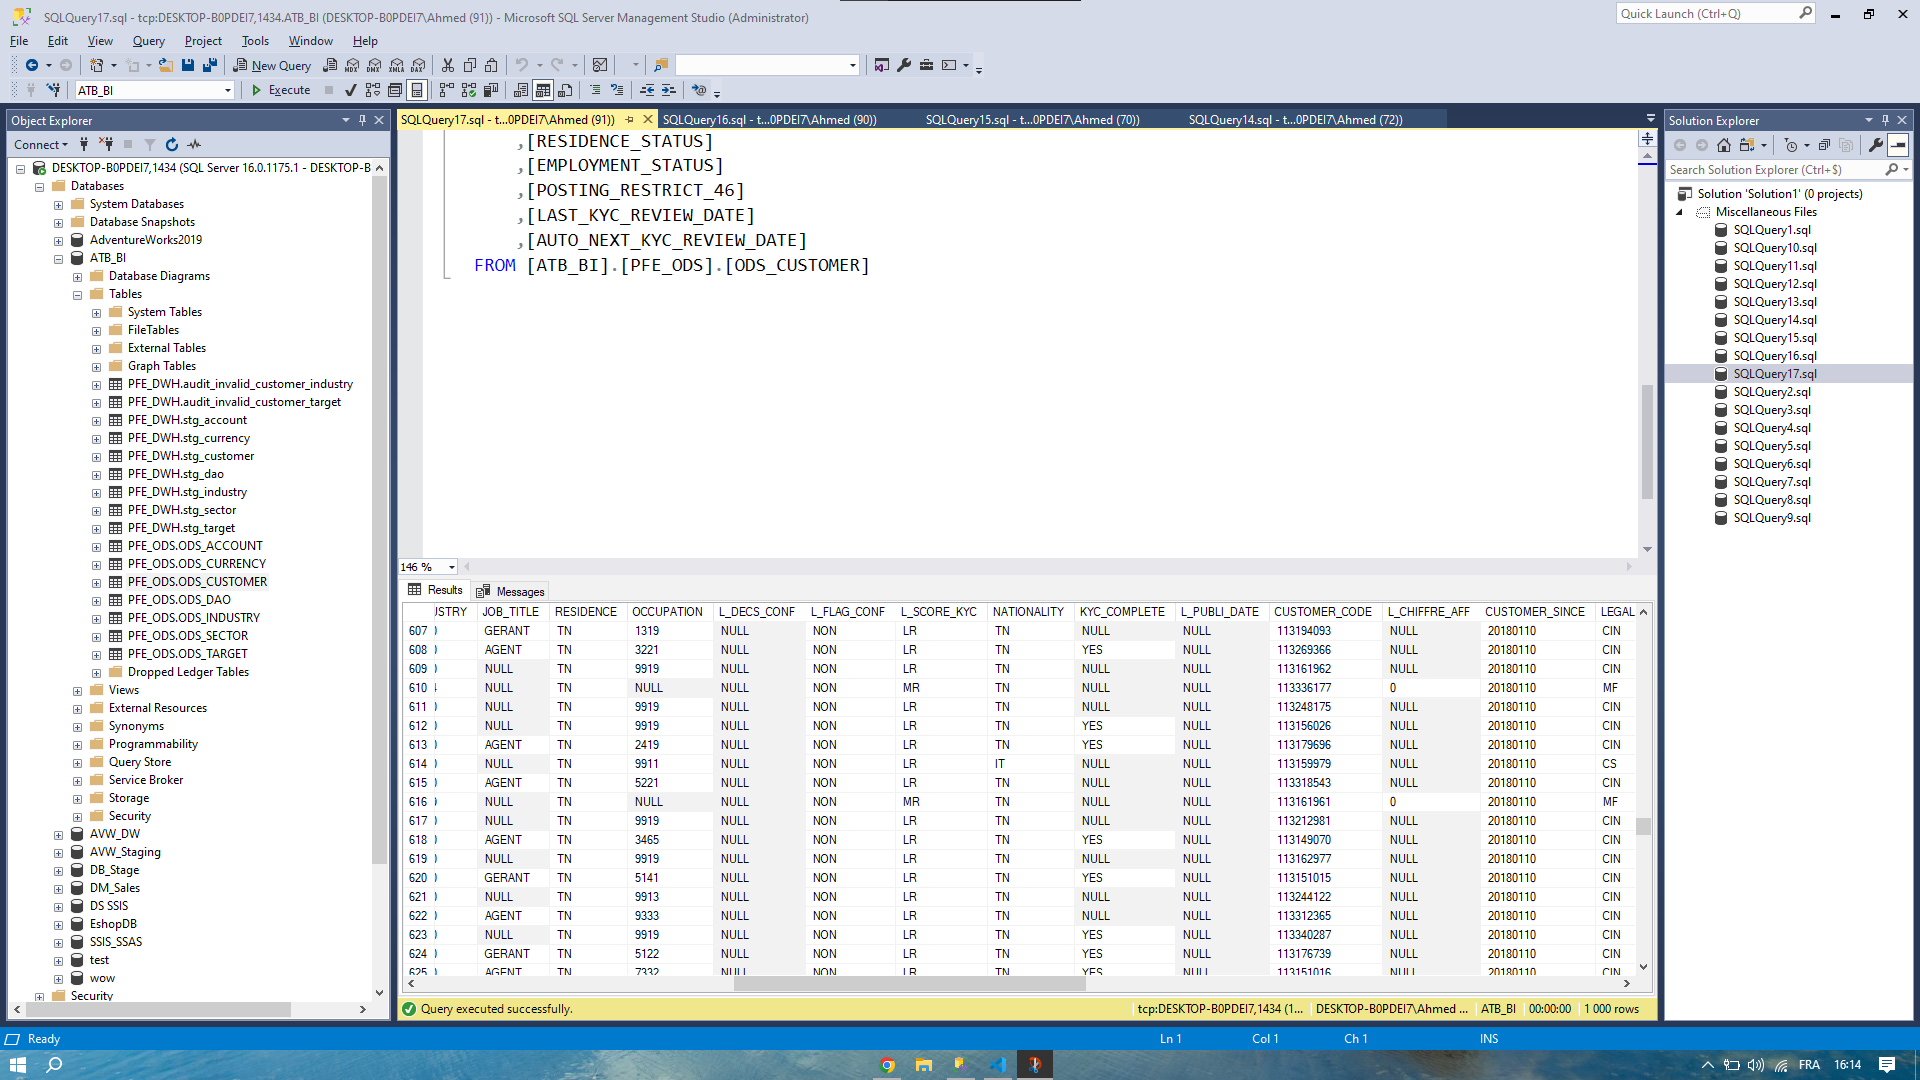
\includegraphics[width=0.85\textwidth]{figures/ods_vs_stg_compare.png}
\caption{SSMS comparison: raw \texttt{ODS\_CUSTOMER.KYC\_COMPLETE} text vs.~staged \texttt{is\_kyc\_complete} bit}
\label{fig:ods_vs_stg_compare}
\end{figure}
Side-by-side SSMS screenshots illustrate the cleaning contract: raw text codes become
consistent bit flags in staging.

\paragraph{Transform phase --- Intermediate (business logic).}
Views in \texttt{PFE\_INTERMEDIATE} enrich profiles and compute risk:
\begin{itemize}
    \item \texttt{int\_customer\_enriched}, \texttt{int\_account\_enriched};
    \item \texttt{int\_customer\_account\_activity} --- per-customer aggregates;
    \item \texttt{int\_customer\_risk\_score} --- three-pillar engine (detailed below).
\end{itemize}

\paragraph{Load phase --- Warehouse materialisation.}
Final tables are materialised in Datawarehouse. Table~\ref{tab:dim-tables}
summarises dimension loads; facts are detailed in Layer~2.

\begin{table}[H]
\centering
\caption{Dimension tables generated by the dbt warehouse load}
\label{tab:dim-tables}
\renewcommand{\arraystretch}{1.2}
\scriptsize
\begin{tabular}{|p{3.0cm}|p{2.6cm}|p{8.2cm}|}
\hline
\rowcolor{blue!15}
\textbf{Table} & \textbf{Surrogate key} & \textbf{Main attributes} \\
\hline
\texttt{dim\_customer} & \texttt{customer\_sk} & Tenure, salary, employment, KYC/PEP/compliance flags, DAO link \\
\hline
\texttt{dim\_dao} & \texttt{dao\_sk} & Officer id, area, name (+ UNKNOWN sentinel) \\
\hline
\texttt{dim\_date} & \texttt{date\_sk} & Calendar attributes (year, month, day,\ldots) \\
\hline
\texttt{dim\_sector} & \texttt{sector\_sk} & Sector code / description \\
\hline
\texttt{dim\_industry} & \texttt{industry\_sk} & Industry code / description \\
\hline
\texttt{dim\_target} & \texttt{target\_sk} & Segment code / description \\
\hline
\texttt{dim\_currency} & \texttt{currency\_sk} & ISO code (+ \texttt{UNK}) \\
\hline
\texttt{dim\_risk\_profile} & \texttt{risk\_profile\_sk} & CRI, FFS, BRS, GRS, tier, scoring date \\
\hline
\end{tabular}
\end{table}

\paragraph{Data quality framework.}
dbt schema tests enforce \texttt{not\_null}/\texttt{unique} on surrogate keys and
\texttt{relationships} from facts to dimensions. Singular SQL tests verify grain
uniqueness and staging parse rates. Failures stop the Airflow run before a broken
dashboard refresh (NFR~5).

%----------------------------------------------------------------------
\section{Baseline Approach: The Three-Pillar Weighted Risk Score}
\label{sec:three_pillar_model}
%----------------------------------------------------------------------
Although the ultimate architectural objective includes Machine Learning for
predictive risk (Release~3), we integrated inside the ELT pipeline a robust
heuristic \textbf{Baseline} serving as reference model and as ground-truth
generator for future supervised learning.

\subsection{Implementation of Business Logic inside the ELT}
In a classical decision architecture, ELT often merely moves data. Here we
enriched it with banking business logic. The SQL model
\texttt{int\_customer\_risk\_score.sql} evaluates three fundamental dimensions and
assigns specific weights according to their critical importance in ATB risk
governance:
\begin{enumerate}
    \item \textbf{Compliance Risk Index --- CRI ($40\%$):} KYC completeness, PEP,
          flags, decisions, posting restrictions, review freshness.
    \item \textbf{Financial Fragility Score --- FFS ($35\%$):} salary, balances,
          overdraft, dependents, unemployment.
    \item \textbf{Behavioural Risk Score --- BRS ($25\%$):} tenure, overdraft
          behaviour, thin balances, stale KYC.
\end{enumerate}

Figure~\ref{fig:three_pillar_tikz} synthesises the scoring flow.

\begin{figure}[H]
\centering
\begin{tikzpicture}[
  font=\scriptsize,
  pill/.style={rectangle, rounded corners=2pt, draw=#1, fill=#1!14, thick,
               align=center, minimum width=3.4cm, minimum height=1.35cm},
  outbox/.style={rectangle, rounded corners=2pt, draw=black!70, fill=gray!12, thick,
              align=center, minimum width=3.6cm, minimum height=1.2cm},
  arr/.style={->, thick}
]
  \node[pill=teal!70!black] (cri) {\textbf{CRI (40\%)}\\KYC / PEP / flags\\$[0,100]$};
  \node[pill=blue!70!black, right=0.45cm of cri] (ffs) {\textbf{FFS (35\%)}\\Salary / balance\\$[0,100]$};
  \node[pill=violet!70!black, right=0.45cm of ffs] (brs) {\textbf{BRS (25\%)}\\Tenure / behaviour\\$[0,100]$};
  \node[outbox, below=1.1cm of ffs] (grs) {\textbf{GRS} $= 0.40\,\mathrm{CRI}+0.35\,\mathrm{FFS}+0.25\,\mathrm{BRS}$};
  \node[outbox, below=0.55cm of grs] (tier) {Tier: LOW / MEDIUM / HIGH / VERY\_HIGH};
  \draw[arr] (cri) |- (grs);
  \draw[arr] (ffs) -- (grs);
  \draw[arr] (brs) |- (grs);
  \draw[arr] (grs) -- (tier);
\end{tikzpicture}
\caption{Three-pillar composite risk scoring flow}
\label{fig:three_pillar_tikz}
\end{figure}

\subsection{Detailed Calculation of Risk Indices}
Each component score ranges from $0$ (lowest risk) to $100$ (highest risk).

\subsubsection{Compliance Risk Index (CRI)}
\begin{equation}
\label{eq:cri}
\mathrm{CRI} = \min\Bigl(100,\;
\Delta_{\mathrm{KYC}}+\Delta_{\mathrm{PEP}}+\Delta_{\mathrm{FLAG}}
+\Delta_{\mathrm{DEC}}+\Delta_{\mathrm{REST}}+\Delta_{\mathrm{DATE}}\Bigr)
\end{equation}
with point increments:
\begin{equation}
\begin{aligned}
\Delta_{\mathrm{KYC}} &= 35\cdot \mathbf{1}[\texttt{is\_kyc\_complete}=0],\\
\Delta_{\mathrm{PEP}} &= 30\cdot \mathbf{1}[\texttt{is\_pep}=1],\\
\Delta_{\mathrm{FLAG}} &= 25\cdot \mathbf{1}[\texttt{is\_compliance\_flagged}=1],\\
\Delta_{\mathrm{DEC}} &= 10\cdot \mathbf{1}[\texttt{has\_compliance\_decision}=1],\\
\Delta_{\mathrm{REST}} &= 15\cdot \mathbf{1}[\texttt{posting\_restriction\_code}\neq\emptyset],\\
\Delta_{\mathrm{DATE}} &=
\begin{cases}
15 & \text{if last KYC date is NULL},\\
10 & \text{if last KYC date }> 365\text{ days},\\
0 & \text{otherwise}.
\end{cases}
\end{aligned}
\end{equation}

\subsubsection{Financial Fragility Score (FFS)}
\begin{equation}
\label{eq:ffs}
\mathrm{FFS} = \min\Bigl(100,\;
\delta_{\mathrm{SAL}}+\delta_{\mathrm{ACC}}+\delta_{\mathrm{OD}}
+\delta_{\mathrm{DEP}}+\delta_{\mathrm{EMP}}\Bigr)
\end{equation}
\begin{equation}
\begin{aligned}
\delta_{\mathrm{SAL}} &= 25\cdot \mathbf{1}[\text{salary}\le 0 \lor \text{NULL}],\\
\delta_{\mathrm{ACC}} &= 20\cdot \mathbf{1}[\texttt{account\_count}=0],\\
\delta_{\mathrm{OD}} &=
\begin{cases}
30 & \text{if total balance}<0,\\
10 & \text{if avg balance}\in[0,500]\ \text{and total}\ge 0,\\
0 & \text{otherwise},
\end{cases}\\
\delta_{\mathrm{DEP}} &= 10\cdot \mathbf{1}[\text{dependents}\ge 4],\\
\delta_{\mathrm{EMP}} &= 20\cdot \mathbf{1}[\text{employment}\in\{\texttt{UNEMPLOYED},\texttt{SANS EMPLOI},\texttt{CHOMEUR}\}].
\end{aligned}
\end{equation}

\subsubsection{Behavioural Risk Score (BRS)}
\begin{equation}
\label{eq:brs}
\mathrm{BRS} = \min\Bigl(100,\;
\gamma_{\mathrm{TEN}}+\gamma_{\mathrm{OD}}+\gamma_{\mathrm{SINGLE}}
+\gamma_{\mathrm{LOW}}+\gamma_{\mathrm{KYC}}\Bigr)
\end{equation}
\begin{equation}
\begin{aligned}
\gamma_{\mathrm{TEN}} &= 25\cdot \mathbf{1}[\text{tenure}<365],\\
\gamma_{\mathrm{OD}} &= 25\cdot \mathbf{1}[\text{any negative-balance account}],\\
\gamma_{\mathrm{SINGLE}} &= 10\cdot \mathbf{1}[\texttt{account\_count}=1],\\
\gamma_{\mathrm{LOW}} &= 15\cdot \mathbf{1}[\text{total balance}<100 \land \texttt{account\_count}>0],\\
\gamma_{\mathrm{KYC}} &= 20\cdot \mathbf{1}[\text{KYC missing or }>730\text{ days}].
\end{aligned}
\end{equation}

\subsubsection{Global Risk Score and tier mapping}
\begin{equation}
\label{eq:grs}
\boxed{\mathrm{GRS} = 0.40\,\mathrm{CRI} + 0.35\,\mathrm{FFS} + 0.25\,\mathrm{BRS}}
\end{equation}
\begin{equation}
\label{eq:tier}
\text{Risk tier} =
\begin{cases}
\texttt{LOW} & \text{if } \mathrm{GRS} < 25,\\
\texttt{MEDIUM} & \text{if } 25 \le \mathrm{GRS} < 50,\\
\texttt{HIGH} & \text{if } 50 \le \mathrm{GRS} < 75,\\
\texttt{VERY\_HIGH} & \text{if } \mathrm{GRS} \ge 75.
\end{cases}
\end{equation}

\begin{table}[H]
\centering
\caption{Justification of the three-pillar weights}
\label{tab:scoring-weights}
\renewcommand{\arraystretch}{1.2}
\scriptsize
\begin{tabular}{|p{3.0cm}|c|p{6.5cm}|p{3.0cm}|}
\hline
\rowcolor{blue!15}
\textbf{Dimension} & \textbf{Weight} & \textbf{Justification} & \textbf{Anchor} \\
\hline
Compliance (CRI) & $40\%$ & Regulatory priority (AML/KYC/PEP) in banking supervision & FATF-aligned monitoring \\
\hline
Financial (FFS) & $35\%$ & Credit / solvency pressure from income and balances & Credit-risk practice \\
\hline
Behavioural (BRS) & $25\%$ & Early-warning relationship signals & Operational risk cues \\
\hline
\end{tabular}
\end{table}

On the production snapshot, average pillars are approximately
$\mathrm{CRI}\approx 10$, $\mathrm{FFS}\approx 34$, $\mathrm{BRS}\approx 38$, giving
$\overline{\mathrm{GRS}}\approx 25.6$. The tier mix is roughly $47.7\%$
\texttt{LOW} and $52.3\%$ \texttt{MEDIUM}, with only a handful of \texttt{HIGH}
profiles --- a realistic retail-heavy distribution.

\subsection{Sensitivity Analysis of Risk Weights}
To validate the retained configuration ($40/35/25$), a sensitivity analysis
compared four weight maps on a large customer sample
(Table~\ref{tab:weights-sensitivity}).

\begin{table}[H]
\centering
\caption{Sensitivity analysis of weighting configurations}
\label{tab:weights-sensitivity}
\renewcommand{\arraystretch}{1.2}
\scriptsize
\begin{tabular}{|p{4.0cm}|c|c|c|}
\hline
\rowcolor{blue!15}
\textbf{Configuration} & \textbf{CRI / FFS / BRS} & \textbf{Alignment with financial stress} & \textbf{Compliance/audit capture} \\
\hline
\textbf{Balanced (selected)} & $\mathbf{40/35/25}$ & $\mathbf{0.835}$ & $\mathbf{91.8\%}$ \\
\hline
Compliance-heavy & $60/20/20$ & $0.621$ & $84.5\%$ \\
\hline
Finance-heavy & $20/60/20$ & $0.784$ & $71.2\%$ \\
\hline
Behaviour-heavy & $20/20/60$ & $0.693$ & $73.4\%$ \\
\hline
\end{tabular}
\end{table}

\paragraph{Analytical interpretation.}
\begin{itemize}
    \item A finance-only weighting tracks overdrafts well but under-detects PEP/KYC
          issues.
    \item A compliance-only weighting misses fragile but formally ``clean'' customers.
    \item The balanced map offers the best compromise for ATB's dual mandate: credit
          monitoring and regulatory vigilance.
\end{itemize}

\subsection{Technical Use and Scoring Results}
The weighted Global Risk Score acts at three strategic levels:
\begin{itemize}
    \item \textbf{ELT batch mode:} scores are materialised nightly into
          \texttt{fact\_customer\_risk} and \texttt{dim\_risk\_profile}.
    \item \textbf{BI restitution:} dashboards consume pre-computed tiers for instant
          cards and charts.
    \item \textbf{Future ML target:} $\mathrm{GRS}\ge 50$ defines the high-risk label
          for Release~3 supervised models, while pillar columns themselves are
          excluded from training features to avoid leakage.
\end{itemize}

%======================================================================
\section{Feature Importance Analysis}
\label{sec:feature_importance}
%======================================================================
To identify the most determining factors of the baseline risk score, we conducted
an in-depth driver analysis. This step is essential to understand which customer
and account attributes most influence GRS  and to validate that the score
encodes the signals managers actually care about.

The analysis follows two complementary approaches:
\begin{enumerate}
    \item \textbf{Composite-feature analysis:} contribution of the engineered pillars
          (CRI, FFS, BRS) to GRS under the official weights.
    \item \textbf{Raw-driver analysis:} empirical association of operational variables
          (KYC completeness, salary, overdraft, tenure,\ldots) with elevated GRS,
          observed through warehouse studies and EDA charts.
\end{enumerate}

\subsection{Results of the Analysis}
\begin{figure}[H]
\centering
\begin{minipage}{0.48\textwidth}
  \centering
  \captionof{table}{Importance of composite pillars in GRS}
  \label{tab:feature-importance-pillars}
  \renewcommand{\arraystretch}{1.2}
  \scriptsize
  \begin{tabular}{|c|l|c|c|}
    \hline
    \textbf{Rank} & \textbf{Feature} & \textbf{Weight} & \textbf{Impact} \\
    \hline
    1 & CRI (Compliance) & $40\%$ & Critical \\
    2 & FFS (Financial) & $35\%$ & Critical \\
    3 & BRS (Behavioural) & $25\%$ & High \\
    \hline
  \end{tabular}
\end{minipage}
\hfill
\begin{minipage}{0.48\textwidth}
  \centering
  \captionof{table}{Empirical ranking of raw risk drivers}
  \label{tab:feature-importance-raw}
  \renewcommand{\arraystretch}{1.2}
  \scriptsize
  \begin{tabular}{|c|l|c|}
    \hline
    \textbf{Rank} & \textbf{Raw driver} & \textbf{Impact} \\
    \hline
    1 & KYC incompleteness & Critical \\
    2 & Missing / low salary & Critical \\
    3 & Overdraft presence & High \\
    4 & Short tenure ($<365$d) & High \\
    5 & Unemployment status & Significant \\
    6 & High dependents ($\ge 4$) & Moderate \\
    7 & Single-account profile & Moderate \\
    \hline
  \end{tabular}
\end{minipage}
\end{figure}

\subsection{Interpretation of Results}
Convergence between the two views is strong:
\begin{itemize}
    \item compliance and financial pillars dominate the formal weight map ($75\%$
          combined), matching the raw dominance of KYC and salary/overdraft signals;
    \item behavioural drivers (tenure, thin balances) remain secondary but
          non-negligible exactly the role assigned to the $25\%$ BRS weight;
    \item portfolio averages ($\mathrm{CRI}$ low, $\mathrm{FFS}$/$\mathrm{BRS}$
          moderate) explain why most customers sit near the LOW/MEDIUM frontier.
\end{itemize}

\subsection{Validation of Architectural Choices}
The driver analysis validates three major design choices:
\begin{enumerate}
    \item storing CRI, FFS and BRS separately in the warehouse (explainability);
    \item dedicating dashboard pages to KYC/PEP and overdraft analytics;
    \item applying DAO filters so branch managers act on the same drivers inside
          their perimeter.
\end{enumerate}

\subsection{Cross-Validation with Exploratory Data Analysis}
These results confirm the exploratory studies exposed on the BI Studies page and
in warehouse statistics reports:

\begin{table}[H]
\centering
\caption{Convergence between EDA observations and driver importance}
\label{tab:eda-importance-convergence}
\renewcommand{\arraystretch}{1.2}
\scriptsize
\begin{tabular}{|p{6.2cm}|p{7.5cm}|}
\hline
\rowcolor{blue!15}
\textbf{EDA / warehouse observation} & \textbf{Validation by driver analysis} \\
\hline
Average CRI $\approx 10$ (generally good KYC) & Incomplete KYC remains the sharpest compliance spike when present. \\
\hline
Average FFS $\approx 34$, BRS $\approx 38$ & Salary weakness and overdraft explain the medium-risk mass. \\
\hline
Tier mix $\approx 47.7\%$ LOW / $52.3\%$ MEDIUM & Score is not collapsed on a single tier; drivers create a realistic split. \\
\hline
Sector $\times$ area heatmaps show hot spots & Geographic + sector concentration justifies constellation joins. \\
\hline
\end{tabular}
\end{table}

\subsection{Implications for Optimisation}
\begin{enumerate}
    \item \textbf{Strategic focus:} keep investing UI and data quality effort on KYC
          and balance/salary fields ($75\%$+ of decision weight).
    \item \textbf{Threshold governance:} the scarcity of \texttt{HIGH}/\texttt{VERY\_HIGH}
          tiers may justify committee review of cut-offs in a later iteration.
    \item \textbf{ML readiness:} raw drivers identified here become candidate features
          for Release~3, while pillar scores stay out of the training matrix.
\end{enumerate}

\subsection{Synthesis}
\begin{itemize}
    \item Compliance ($40\%$) and Financial ($35\%$) pillars dominate GRS by design
          and by empirical evidence.
    \item KYC completeness, salary, overdraft and tenure are the primary actionable
          levers for managers.
    \item Behavioural signals add early-warning colour without drowning regulatory
          priority.
\end{itemize}

%----------------------------------------------------------------------
\subsection{Layer 2: Data Warehouse (SQL Server \texttt{PFE\_DWH})}
%----------------------------------------------------------------------
This layer is the \textbf{central persistence zone} of the BI architecture. It
stores the eight dimensions and two facts of the constellation modelled in
Phase~2.

\paragraph{Integrity pattern (sentinel UNKNOWN).}
Dirty operational references (missing officer, unknown currency,\ldots) are not
dropped. Each dimension contains an UNKNOWN row (surrogate $-1$ or code
\texttt{UNK}); fact loaders use \texttt{LEFT JOIN} + \texttt{COALESCE(..., -1)}.
Production validation reports \textbf{zero NULL foreign keys} across
$281{,}960$ fact rows ($145{,}284 + 136{,}676$).

\begin{table}[H]
\centering
\caption{Warehouse fact volumetry and integrity audit}
\label{tab:dwh_audit}
\renewcommand{\arraystretch}{1.2}
\scriptsize
\begin{tabular}{|p{4.0cm}|c|c|c|}
\hline
\rowcolor{blue!15}
\textbf{Table} & \textbf{Rows} & \textbf{NULL FKs} & \textbf{Grain} \\
\hline
\texttt{fact\_account} & $145{,}284$ & $0$ & 1 row / account \\
\hline
\texttt{fact\_customer\_risk} & $136{,}676$ & $0$ & 1 row / customer / scoring date \\
\hline
\textbf{Total facts} & $\mathbf{281{,}960}$ & $\mathbf{0}$ & --- \\
\hline
\end{tabular}
\end{table}

\paragraph{Connectivity.}
Streamlit and quality jobs access \texttt{PFE\_DWH} through SQLAlchemy with
connection pooling (typically five active connections), avoiding handshake storms
during concurrent dashboard use.

%----------------------------------------------------------------------
\subsection{Layer 3: Business Layer (Aggregations and Statistical Calculations)}
%----------------------------------------------------------------------
The business layer is the \textbf{analytical engine} bridging warehouse tables and
Streamlit visuals. Access is centralised in \texttt{dashboard/loaders.py}, with
functions decorated by \texttt{@st.cache\_data}. Once DataFrames are in memory,
pages compute KPIs via vectorised Pandas/SQL aggregations without redundant
round-trips.

\begin{table}[H]
\centering
\caption{Algorithmic translation of steering KPIs}
\label{tab:kpi-calculs}
\renewcommand{\arraystretch}{1.2}
\scriptsize
\begin{tabular}{|p{3.2cm}|p{5.5cm}|p{5.5cm}|}
\hline
\rowcolor{blue!15}
\textbf{Displayed KPI} & \textbf{Aggregation logic} & \textbf{Threshold / meaning} \\
\hline
High-risk customers & Count where $\mathrm{GRS}\ge 50$ & Amber/red follow-up band \\
\hline
Overdraft accounts & Count where balance $<0$ & Solvency pressure \\
\hline
Incomplete KYC & Count where \texttt{is\_kyc\_complete}=0 & Compliance backlog \\
\hline
PEP population & Count where \texttt{is\_pep}=1 & Enhanced due diligence \\
\hline
Portfolio averages & Mean of GRS / CRI / FFS / BRS & Health benchmarks \\
\hline
\end{tabular}
\end{table}

Nightly rebuild is orchestrated by Airflow DAG \texttt{atb\_master\_pipeline}
(schedule \texttt{0 2 * * *}): Airbyte sync $\rightarrow$ dbt build/test
$\rightarrow$ data-quality report ($\rightarrow$ optional weekly ML train).

%----------------------------------------------------------------------
\subsection{Layer 4: Presentation (Interactive Streamlit Interface)}
%----------------------------------------------------------------------
The front-end, developed in \textbf{Python with Streamlit}, restitutes the
intelligence generated by the data layers. Its architecture rests on three
advanced software pillars:

\begin{itemize}
    \item \textbf{Dynamic routing and security (RBAC):} after authentication, the
          interface adapts to \texttt{DG\_CENTRAL}, \texttt{CHEF\_CONFORMITE},
          \texttt{CHEF\_AGENCE}, \texttt{ANALYSTE\_RISQUE} or \texttt{AUDIT}
          (read-only). Branch Managers receive DAO-scoped SQL automatically.
    \item \textbf{Design system:} reusable KPI cards, Plotly theme harmonisation,
          bilingual labels (FR/EN), and consistent risk colours.
    \item \textbf{Session state:} \texttt{st.session\_state} preserves filters and
          navigation context without useless database reloads.
\end{itemize}

\begin{figure}[H]
\centering
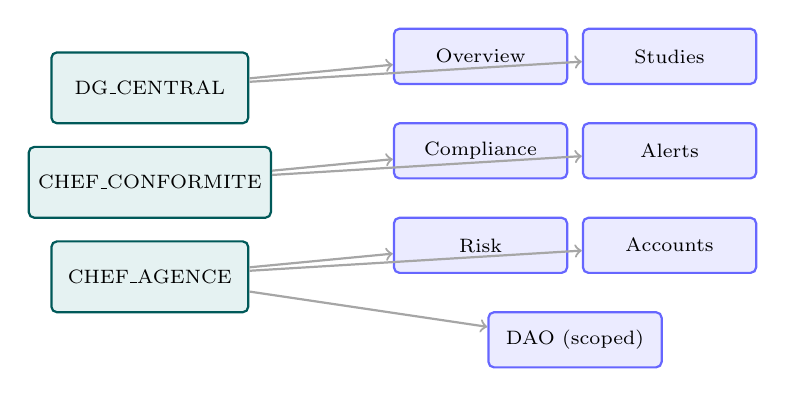
\begin{tikzpicture}[
  font=\scriptsize,
  role/.style={rectangle, rounded corners=2pt, draw=teal!70!black, fill=teal!10,
               thick, align=center, minimum width=2.5cm, minimum height=0.9cm},
  page/.style={rectangle, rounded corners=2pt, draw=blue!60, fill=blue!8,
               thick, align=center, minimum width=2.2cm, minimum height=0.7cm},
  arr/.style={->, thick, gray!70}
]
  \node[role] (dg) at (0,2.2) {DG\_CENTRAL};
  \node[role] (cc) at (0,1.0) {CHEF\_CONFORMITE};
  \node[role] (ag) at (0,-0.2) {CHEF\_AGENCE};
  \node[page] (ov) at (4.2,2.6) {Overview};
  \node[page] (st) at (6.6,2.6) {Studies};
  \node[page] (co) at (4.2,1.4) {Compliance};
  \node[page] (al) at (6.6,1.4) {Alerts};
  \node[page] (rk) at (4.2,0.2) {Risk};
  \node[page] (ac) at (6.6,0.2) {Accounts};
  \node[page] (dao) at (5.4,-1.0) {DAO (scoped)};
  \draw[arr] (dg) -- (ov);
  \draw[arr] (dg) -- (st);
  \draw[arr] (cc) -- (co);
  \draw[arr] (cc) -- (al);
  \draw[arr] (ag) -- (rk);
  \draw[arr] (ag) -- (ac);
  \draw[arr] (ag) -- (dao);
\end{tikzpicture}
\caption{Routing sketch for roles to analytical pages}
\label{fig:rbac_routing_tikz}
\end{figure}

\subsection{Interactive Dashboard: Architecture of Analytical Views}
The dashboard is a multi-page Streamlit application. Think of it as several
``rooms'' for different questions: a national overview for General Management, a
compliance room for the CCO, a risk deep-dive, account analytics, and a full
\textbf{dimensional catalog} so analysts can explore every Kimball dimension on
its own. Table~\ref{tab:vues-analytiques} summarises the Release~2 analytical
scope.

\begin{table}[H]
\centering
\caption{Architecture of analytical dashboard views (GIMSI Phase~3 presentation)}
\label{tab:vues-analytiques}
\renewcommand{\arraystretch}{1.2}
\scriptsize
\begin{tabular}{|p{3.2cm}|p{3.2cm}|p{7.4cm}|}
\hline
\rowcolor{blue!15}
\textbf{Module (file)} & \textbf{Analytical axis} & \textbf{KPIs and visualisations} \\
\hline
\texttt{overview.py} & Macro portfolio & Customers, accounts, total balance, avg GRS, high-risk \%, overdraft \%, risk pie, sector bars, drill-down CSV/PDF \\
\hline
\texttt{studies.py} & Cross-dimensional BI & KYC vs risk, salary vs GRS scatter, sector$\times$area heatmap, tenure bands, employment studies \\
\hline
\texttt{compliance.py} & Regulatory monitoring & PEP \%, KYC completion \%, flagged customers, overdue KYC queue \\
\hline
\texttt{alert\_inbox.py} & Operational follow-up & Prioritised alert count, severity mix, export pack \\
\hline
\texttt{risk.py} & Three-pillar deep dive & Mean CRI/FFS/BRS, tier mix, pillar histograms, customer fiche \\
\hline
\texttt{accounts.py} & Balance / overdraft & Total balance, overdraft rate, age bands, balance histogram \\
\hline
\texttt{comparison.py} & Side-by-side comparison & Two DAO areas or two sectors: customers, accounts, balance, avg risk, high-risk \%, overdraft \%, grouped bars \\
\hline
\texttt{dim\_customer\_page.py} & Customer dimension & See Table~\ref{tab:dim_dashboard_kpis} \\
\hline
\texttt{dim\_dao\_page.py} & Branch / DAO network & Branch count, areas, balance \& overdraft by area, risk scatter \\
\hline
\texttt{dim\_sector\_page.py} & Economic sectors & Top sector by accounts, highest avg risk, max overdraft \% \\
\hline
\texttt{dim\_industry\_page.py} & Industries & Industry volume, risk bubble, account exposure \\
\hline
\texttt{dim\_target\_page.py} & Segments & Largest segment, highest-risk segment, top balance segment \\
\hline
\texttt{dim\_currency\_page.py} & FX reference & Currency count, exposure, overdraft \& risk by currency \\
\hline
\texttt{dim\_date\_page.py} & Calendar / vintage & Days covered, openings by year, balance by vintage \\
\hline
\end{tabular}
\end{table}

%----------------------------------------------------------------------
\subsubsection*{Executive, risk and compliance pages}
%----------------------------------------------------------------------
Figure~\ref{fig:dashboard_overview} is the national entry point. In everyday
language: the top cards answer ``how big is the book and how healthy is it?'',
while the charts answer ``where does the risk sit?''. The page articulates four
zones:
\begin{enumerate}
    \item \textbf{Navigation sidebar:} BI groups, language toggle, AI explanation
          controls;
    \item \textbf{System status / freshness:} last warehouse load timestamp;
    \item \textbf{Global KPIs:} customers, accounts, balances, average risk,
          high-risk share, overdraft share;
    \item \textbf{Analytical charts:} risk-tier composition, three-pillar averages
          by tier, currency treemap and top sectors by balance, with CSV/PDF export.
\end{enumerate}

\begin{figure}[H]
\centering
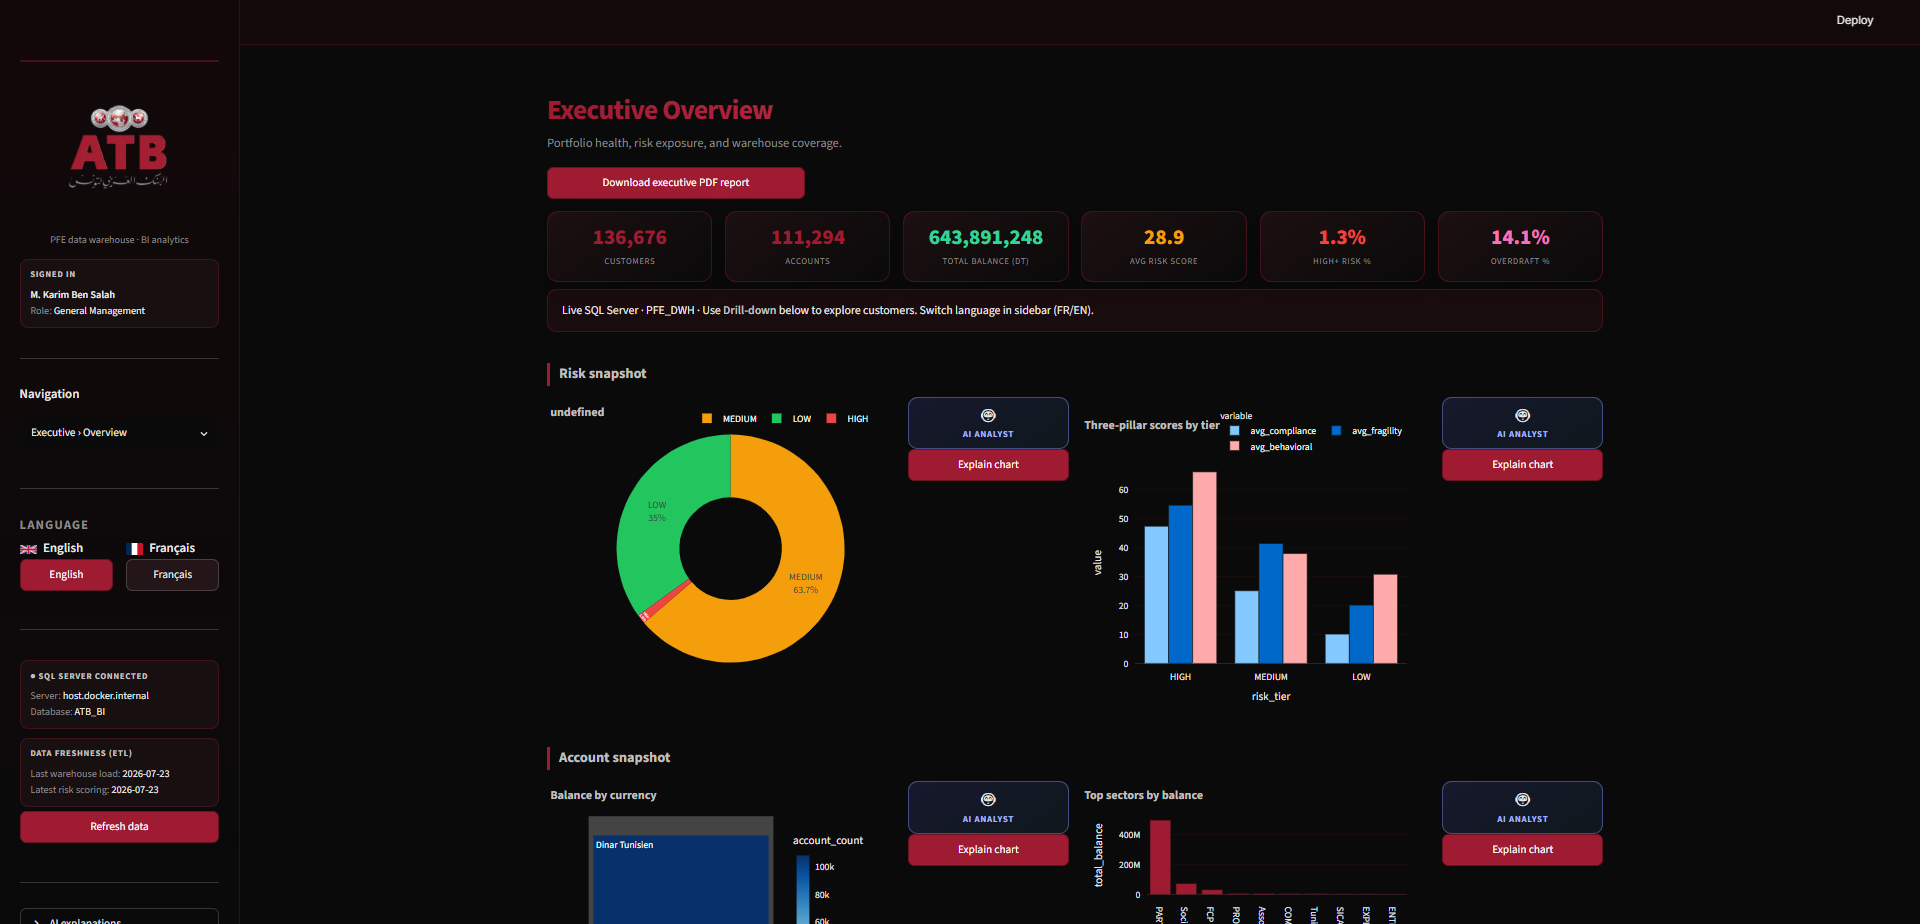
\includegraphics[width=0.88\textwidth]{figures/dash_overview_kpis.png}
\caption{Executive Overview portfolio KPIs, risk distribution and sector exposure}
\label{fig:dashboard_overview}
\end{figure}
\noindent Six headline cards (136{,}676 customers, 111{,}294 accounts,
643~M~DT balance, avg GRS 28.9, 1.3\% high-risk, 14.1\% overdraft) sit above a
risk-tier donut, three-pillar bars by tier, a currency treemap and top sectors
by balance. The sidebar confirms SQL Server connectivity and warehouse freshness.

\begin{figure}[H]
\centering
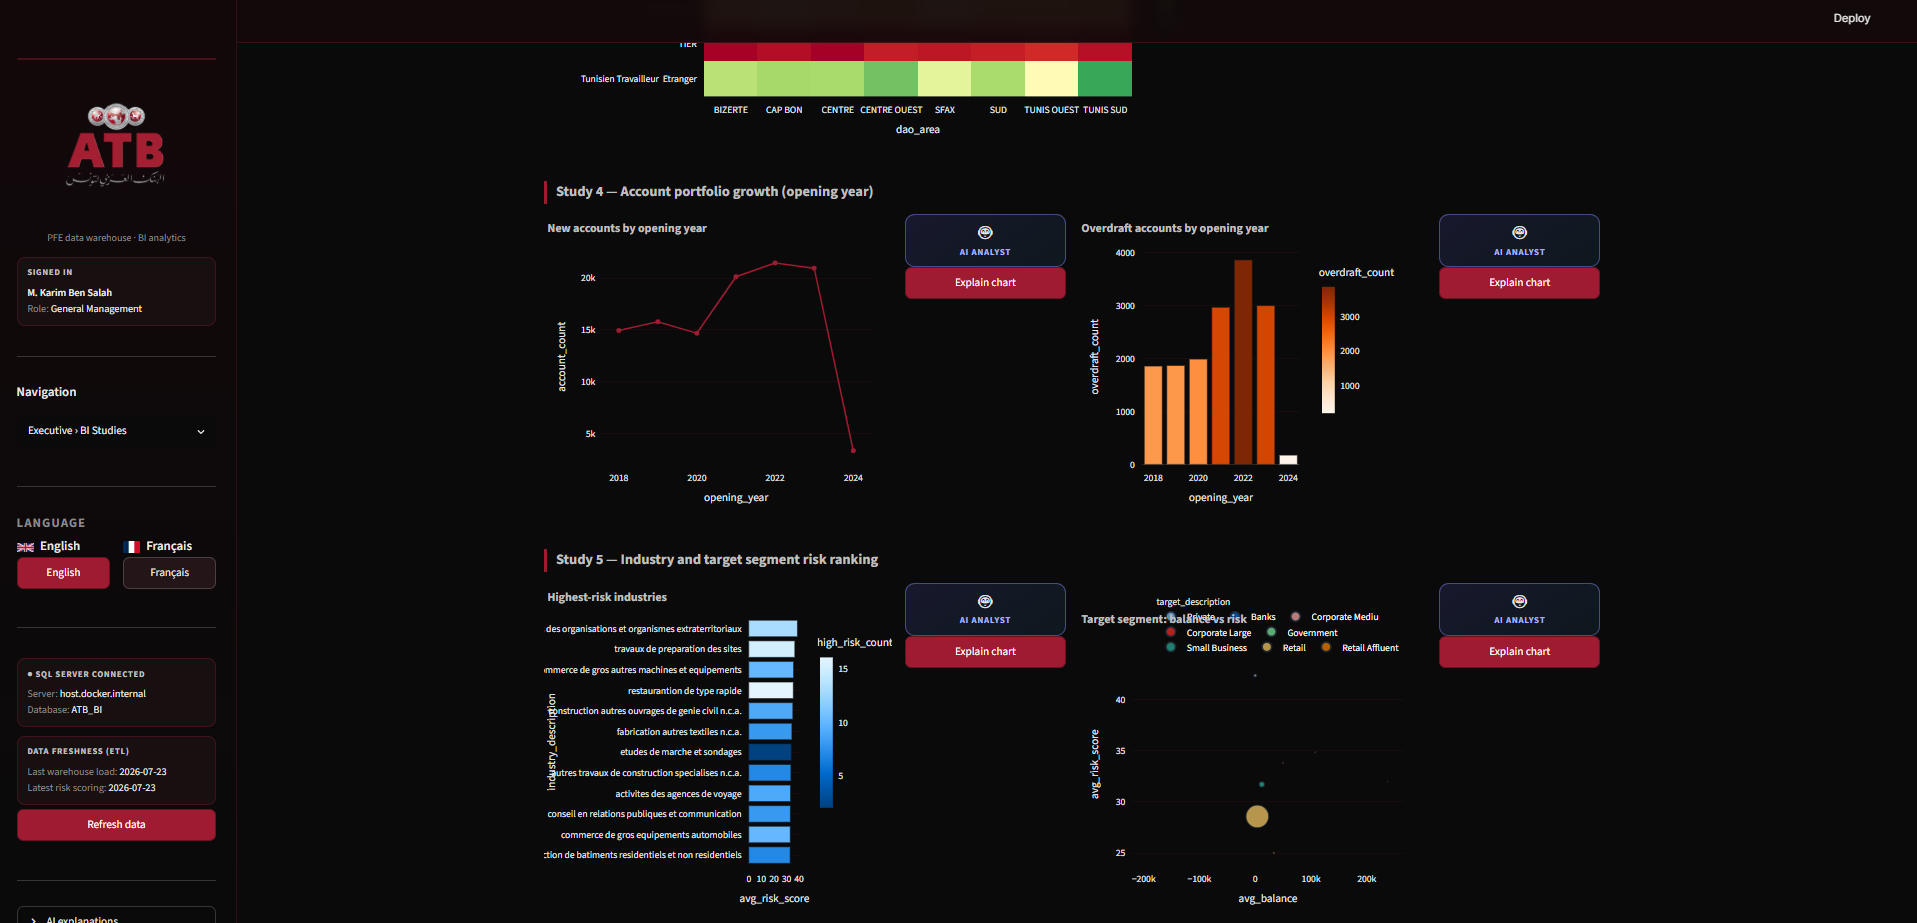
\includegraphics[width=0.88\textwidth]{figures/dash_studies.png}
\caption{BI Studies page account openings by vintage and industry, segment, risk}
\label{fig:dash_studies}
\end{figure}
\noindent Study panels deepen the overview: new and overdraft
accounts by opening year show portfolio growth, while highest-risk industries
and a balance-vs-risk scatter by target segment highlight concentration pockets
for committee follow-up.

\begin{figure}[H]
\centering
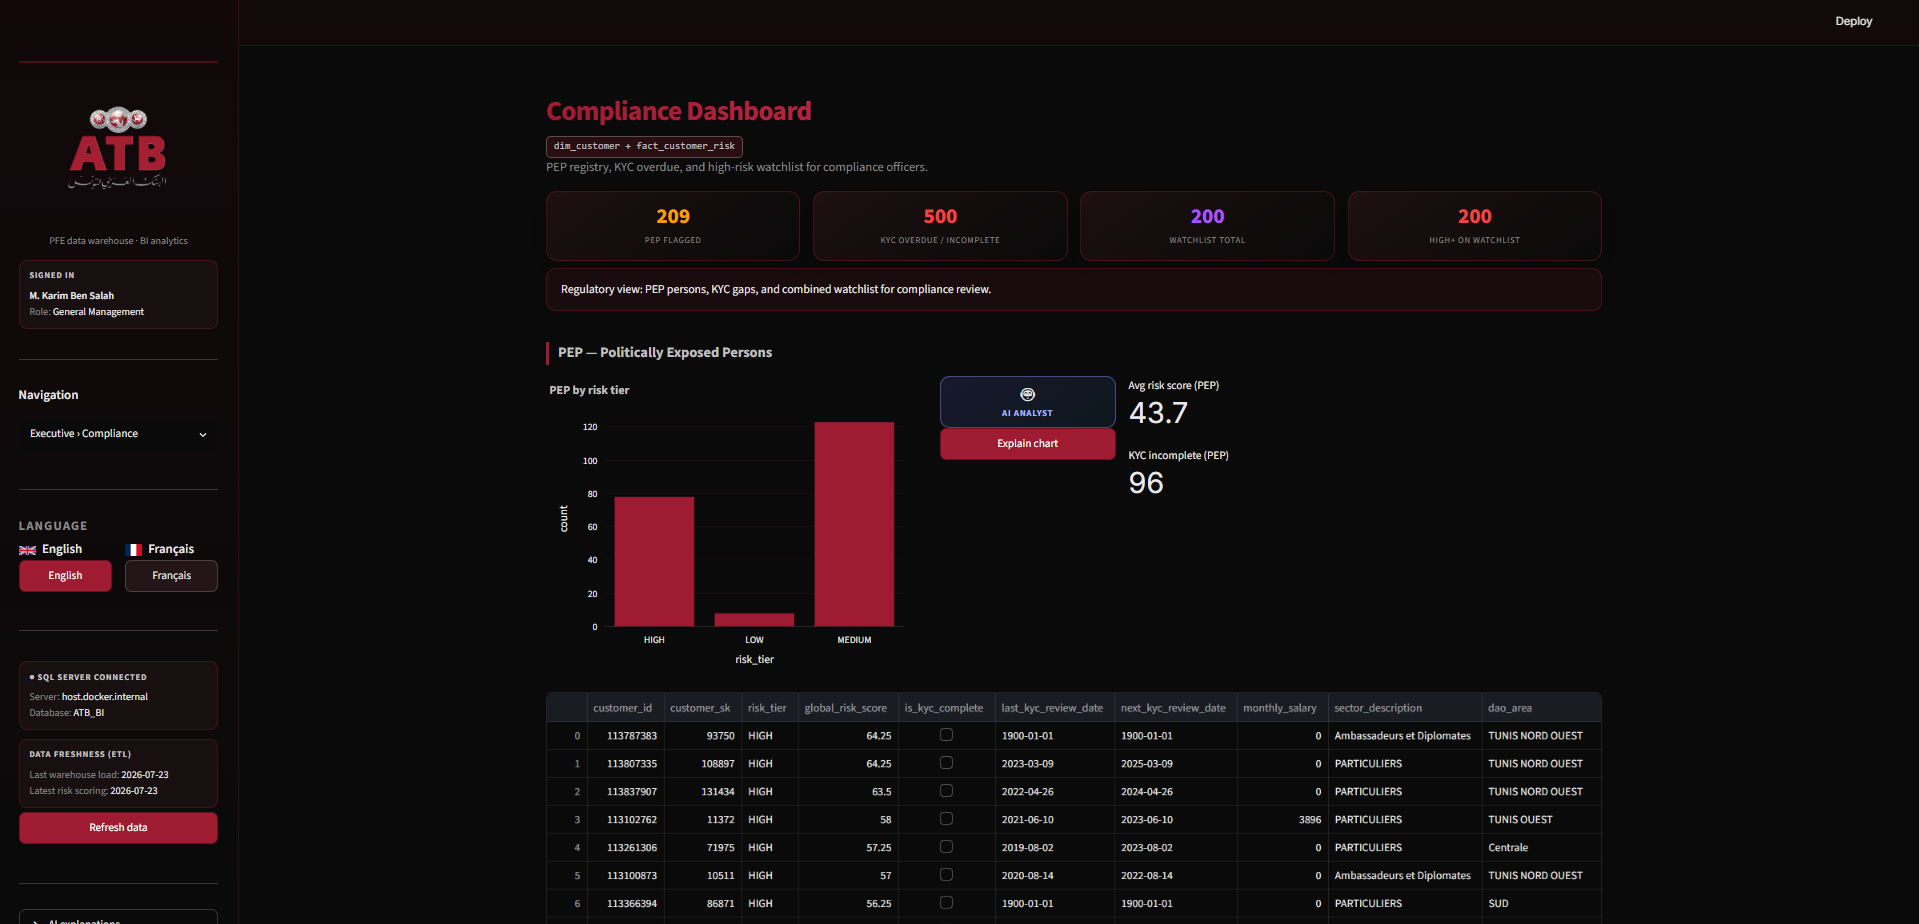
\includegraphics[width=0.88\textwidth]{figures/dash_compliance.png}
\caption{Compliance Dashboard --- PEP registry, KYC overdue and high-risk watchlist}
\label{fig:dash_compliance}
\end{figure}
\noindent Compliance officers see PEP flagged (209), KYC overdue
(500) and watchlist totals at a glance, with PEP-by-tier bars and a row-level
customer table joining \texttt{Dimension customer} to \texttt{fact customer risk}
for enhanced due diligence.

\begin{figure}[H]
\centering
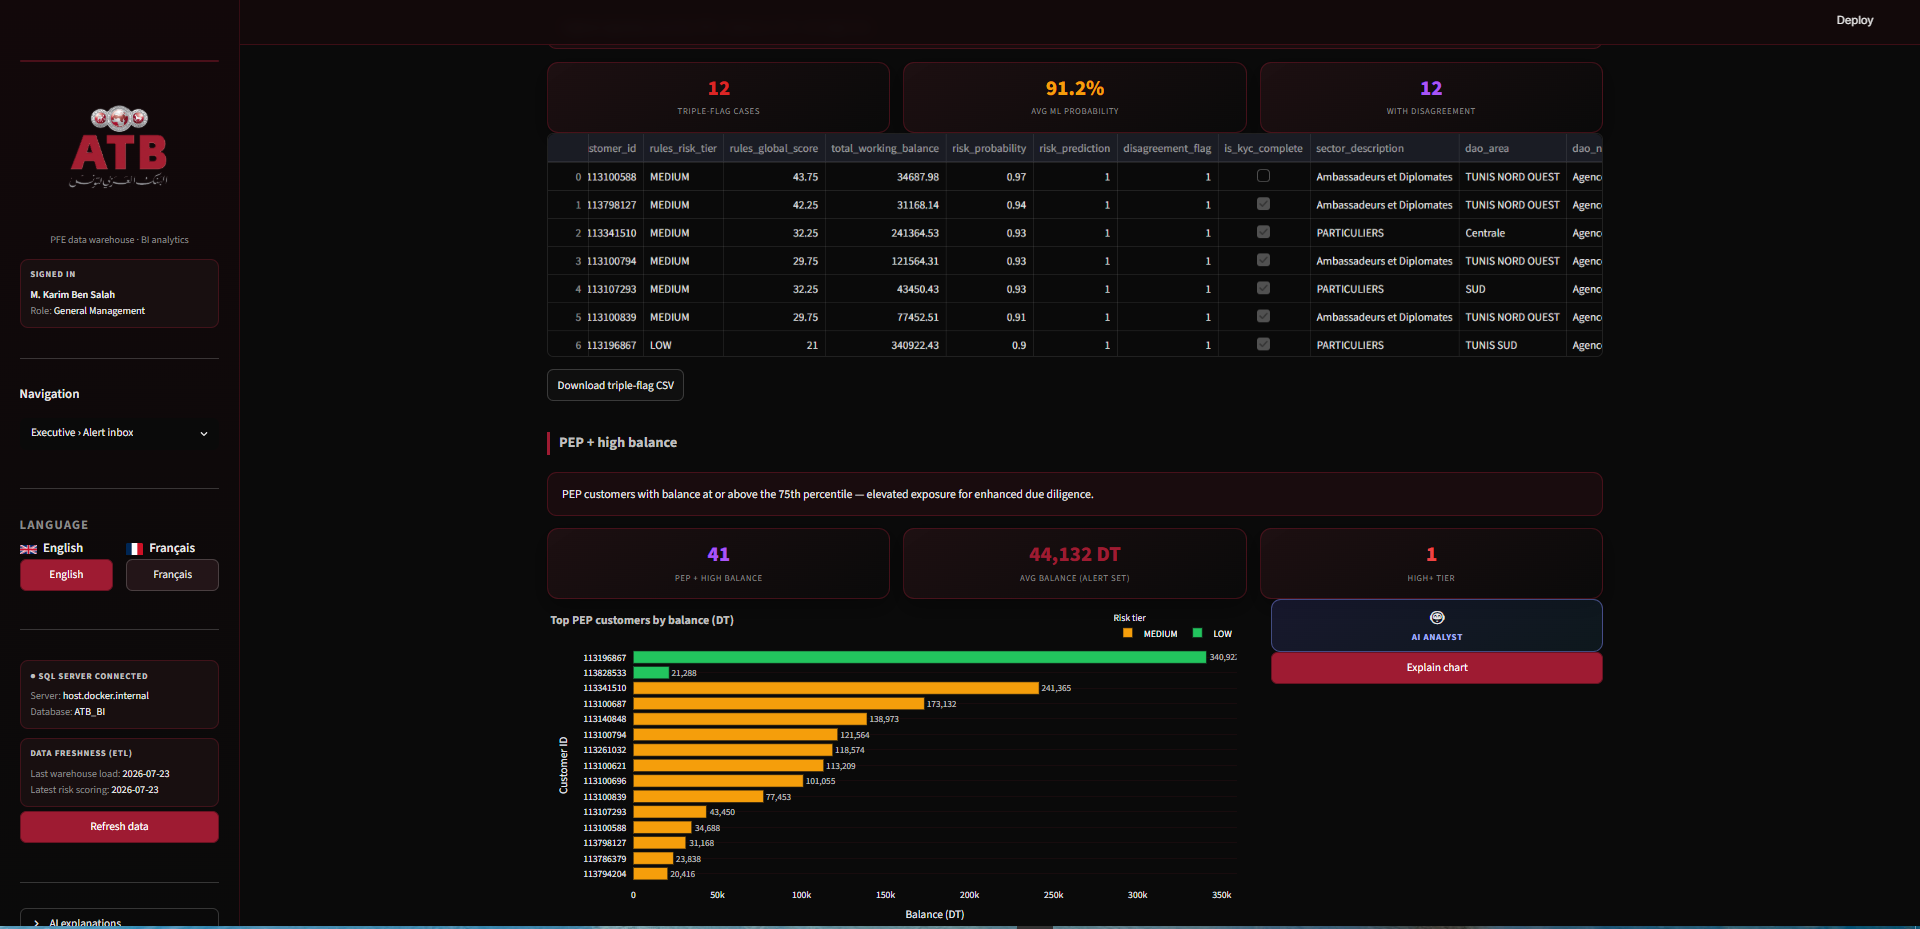
\includegraphics[width=0.88\textwidth]{figures/dash_alert_inbox.png}
\caption{Alert inbox triple-flag cases, ML disagreement and PEP high-balance}
\label{fig:dash_alert_inbox}
\end{figure}
\noindent The inbox prioritises cases where rules, KYC and ML
signals coincide (triple-flag), surfaces ML/rules disagreements for review, and
lists PEP customers with balances above the 75th percentile ready for CSV
export to the compliance team.

\begin{figure}[H]
\centering
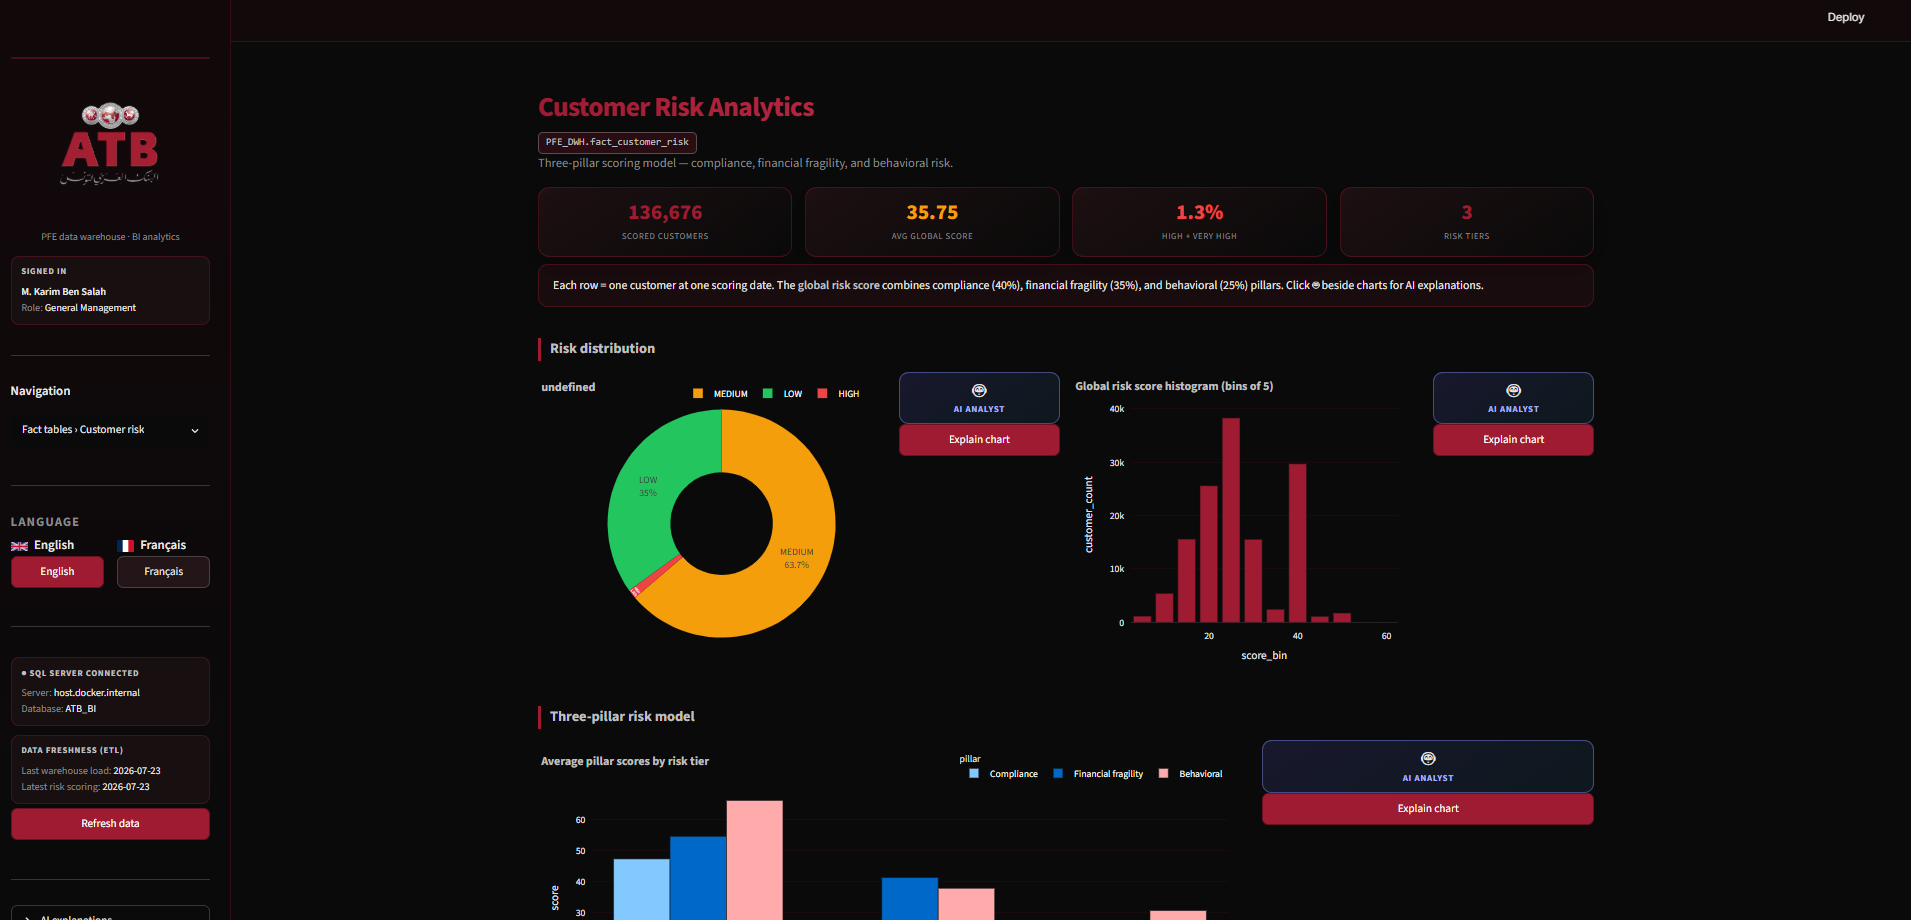
\includegraphics[width=0.88\textwidth]{figures/dash_risk_pillars.png}
\caption{Customer Risk Analytics GRS distribution and three-pillar breakdown}
\label{fig:dash_risk_pillars}
\end{figure}
\noindent Built on the 40/35/25 weighting (compliance /
financial fragility / behavioural), the page shows tier mix (1.3\% high), the
GRS histogram and average pillar scores by tier explaining \emph{why} a
customer lands in HIGH rather than only showing the final score.

\begin{figure}[H]
\centering
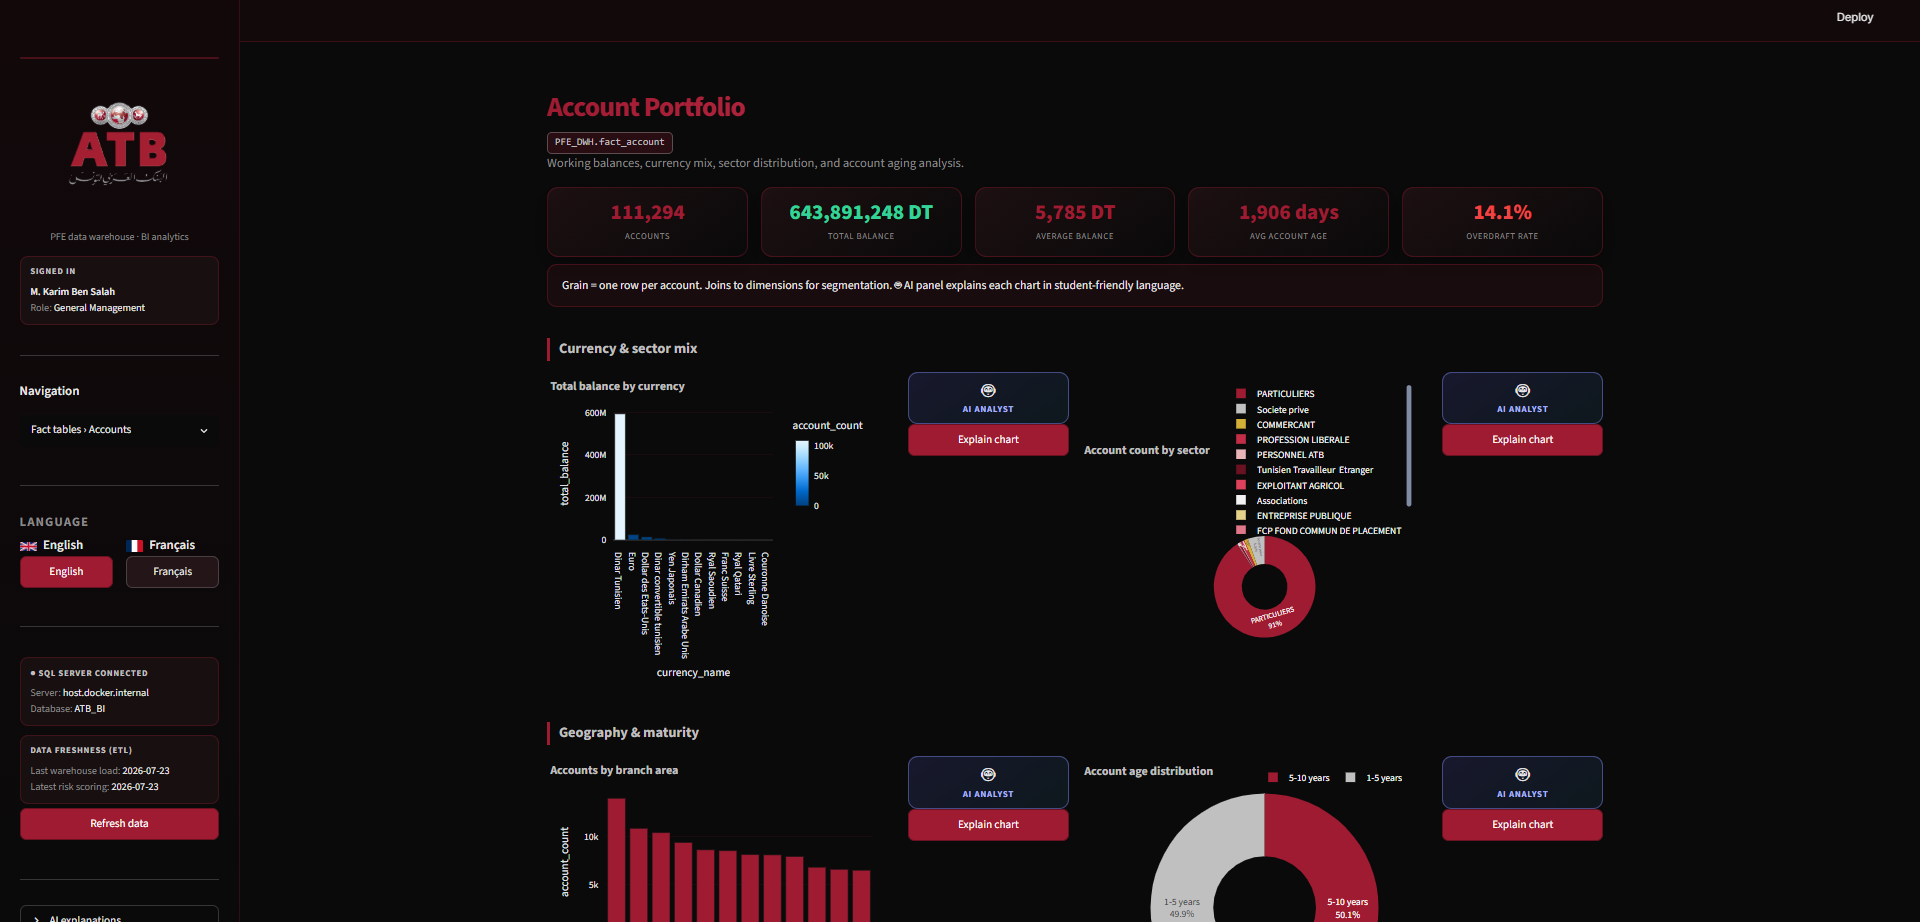
\includegraphics[width=0.88\textwidth]{figures/dash_accounts.png}
\caption{Account Portfolio balances, currency mix and sectors}
\label{fig:dash_accounts}
\end{figure}
\noindent Grain is one row per account from
\texttt{fact\_account}: KPIs cover volume, total/average balance, age and
overdraft rate; charts break exposure by currency and sector, then geography
and account-age bands.

\paragraph{DAO / sector comparison (US~13).}
Beyond single-dimension pages, the dashboard exposes a dedicated
\textbf{Comparison} view so Central General Management
and risk analysts can confront two entities side by side. The user selects the
comparison mode \emph{DAO area} or \emph{sector} then picks Entity~A and
Entity~B. The page returns a metric table (customers, accounts, total balance,
average GRS, high-risk share, overdraft rate) with deltas, a grouped bar chart,
and complementary customer-mix / average-risk visuals. This answers US~13
directly: mathematical comparison of risk levels by geographic zone or by
economic sector without exporting data to Excel.

% --- SCREENSHOT PLACEHOLDER: Save your screenshot as report/figures/Comparisim_mode.png and uncomment below:
%\begin{figure}[H]
%\centering
%\includegraphics[width=0.55\textwidth]{figures/Comparisim_mode.png}
%\caption{Streamlit Comparison page side-by-side sectors: metric deltas and grouped bars}
%\label{fig:dash_comparison_dao}
%\end{figure}
\noindent Figure~\ref{fig:dash_comparison_dao} will show the live
Comparison screen once the screenshot is inserted: two DAO areas selected in
the header, the delta table in the centre, and the Plotly grouped bars below the same panel also supports an optional Gemini ``Explain chart'' call.

\paragraph{AI-generated chart explanations.}
Selected Plotly charts expose an ``Explain chart'' panel powered by Google Gemini. On API failure, a deterministic template fallback
still returns a usable sentenceso FR~6 stays available even offline.
\begin{figure}[H]
\centering
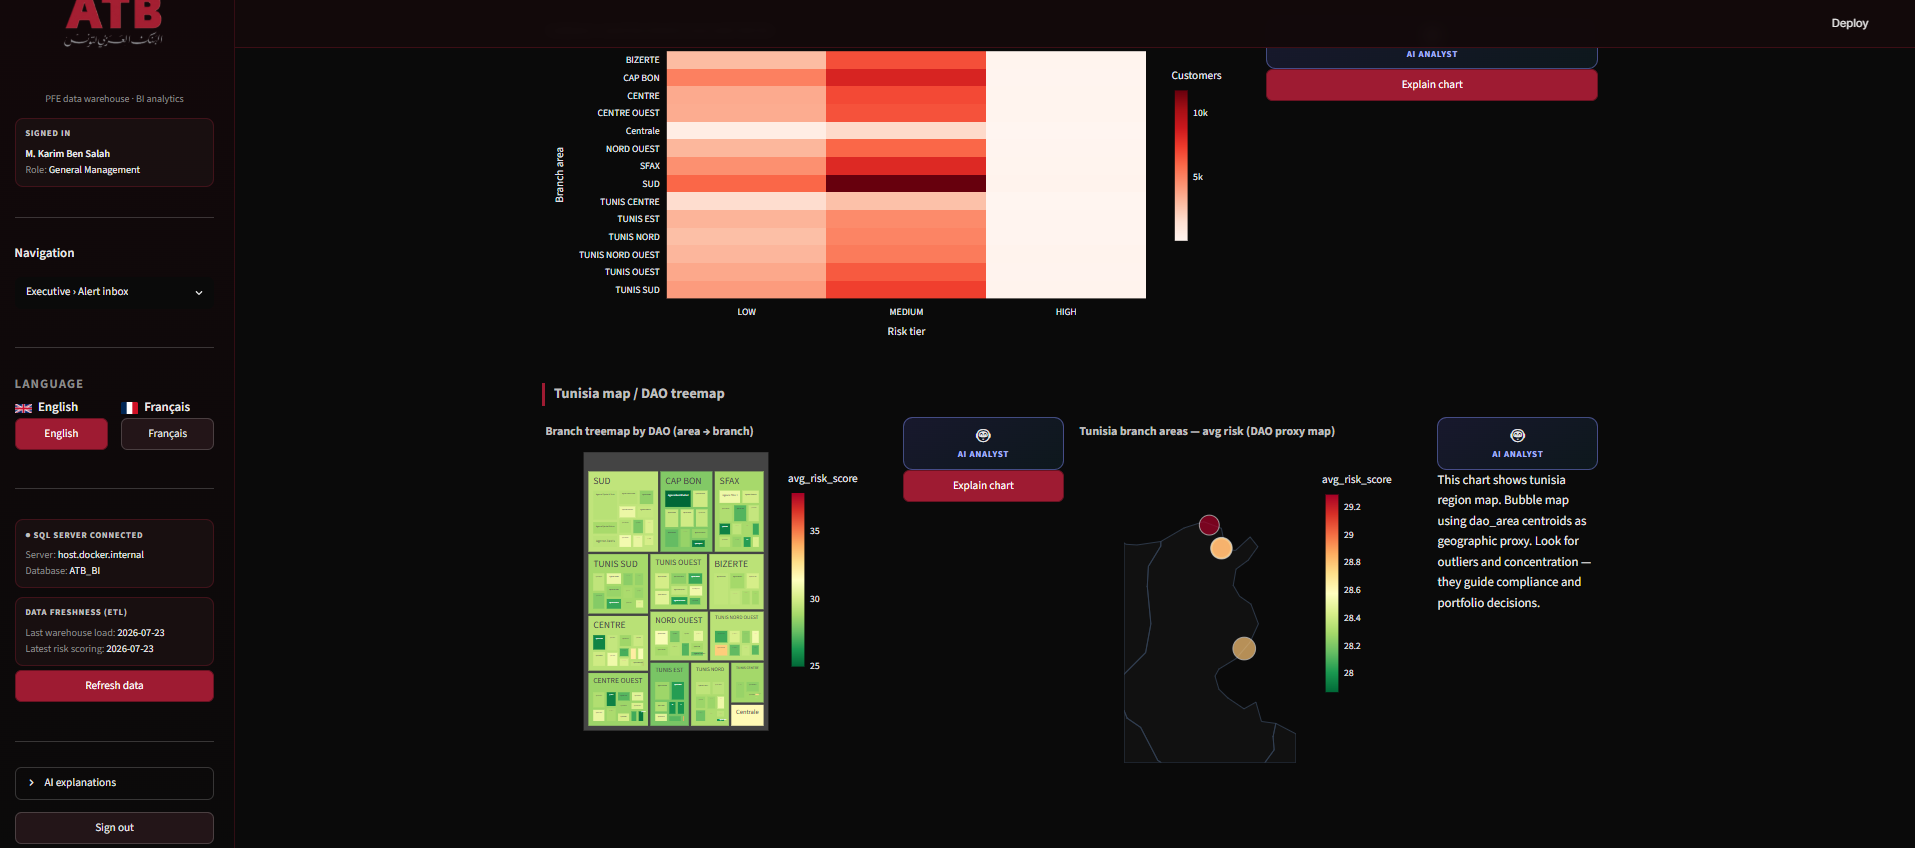
\includegraphics[width=0.85\textwidth]{figures/dash_ai_explain.png}
\caption{Gemini AI explanation panel beside a Plotly chart}
\label{fig:dash_ai_explain}
\end{figure}
\noindent Each chart can request a plain-language interpretation
calibrated to the user's role; the panel appears beside the visualisation so
managers never leave the analytical context.

%----------------------------------------------------------------------
\subsubsection*{Dimension dashboards (Kimball catalog in Streamlit)}
%----------------------------------------------------------------------
A constellation warehouse is only half useful if managers only ever see facts.
Release~2 therefore exposes \textbf{one Streamlit page per major dimension}.
Each page joins the dimension to \texttt{fact account} and/or
\texttt{fact customer risk}, so a ``dimension view'' is never a static
dictionary it is an analytical lens.

\begin{table}[H]
\centering
\caption{Dimension dashboard KPIs and charts implemented in Streamlit}
\label{tab:dim_dashboard_kpis}
\renewcommand{\arraystretch}{1.2}
\scriptsize
\begin{tabular}{|p{2.8cm}|p{5.0cm}|p{6.4cm}|}
\hline
\rowcolor{blue!15}
\textbf{Dimension page} & \textbf{Header KPIs} & \textbf{Main charts / tables} \\
\hline
\textbf{Customers} & Total customers; avg salary (DT); avg tenure (days); KYC complete \%; PEP \%; compliance-flagged \% & Gender pie; employment bars; compliance flag pie; KYC$\times$tier bars; salary bands; tenure bands; marital pie; sector bars; residence \\
\hline
\textbf{DAO / Branches} & Branch (DAO) count; area count; department count; top area by balance & Area treemap; branch counts; balance by area; overdraft by area; risk vs volume scatter; branch directory \\
\hline
\textbf{Sectors} & Sector count; top sector by accounts; highest avg risk; max overdraft \% & Catalog bars; risk ranking; balance by sector; overdraft rate; accounts$\times$risk bubble; high-risk counts \\
\hline
\textbf{Industries} & Industry count; top industries by customers/accounts; risk focus & Concentration bars; account exposure; risk-vs-volume bubble \\
\hline
\textbf{Target segments} & Segment count; largest segment; highest-risk segment; top balance segment & Segment mix pie; avg risk by segment; balance \& accounts by segment; balance-vs-risk scatter \\
\hline
\textbf{Currencies} & Currency count; exposure totals; overdraft focus & Reference table; account exposure; overdraft \& risk by FX; balance treemap \\
\hline
\textbf{Calendar} & Calendar days; years covered; min/max year & Dates per year; weekend split; month/quarter seasonality; openings by year; balance by vintage \\
\hline
\end{tabular}
\end{table}

These dimension pages matter for three concrete reasons:
\begin{itemize}
    \item \textbf{Traceability:} a committee can open \texttt{dim\_sector} and see
          exactly which economic activities concentrate overdraft or high GRS;
    \item \textbf{Branch governance:} \texttt{dim\_dao} is the geographic cockpit
          behind US~06 the same page becomes DAO-scoped for a Branch Manager;
    \item \textbf{Feature discovery for Release~3:} salary bands, tenure bands and
          KYC flags visible here are the raw drivers later reused by ML features.
\end{itemize}

\begin{figure}[H]
\centering
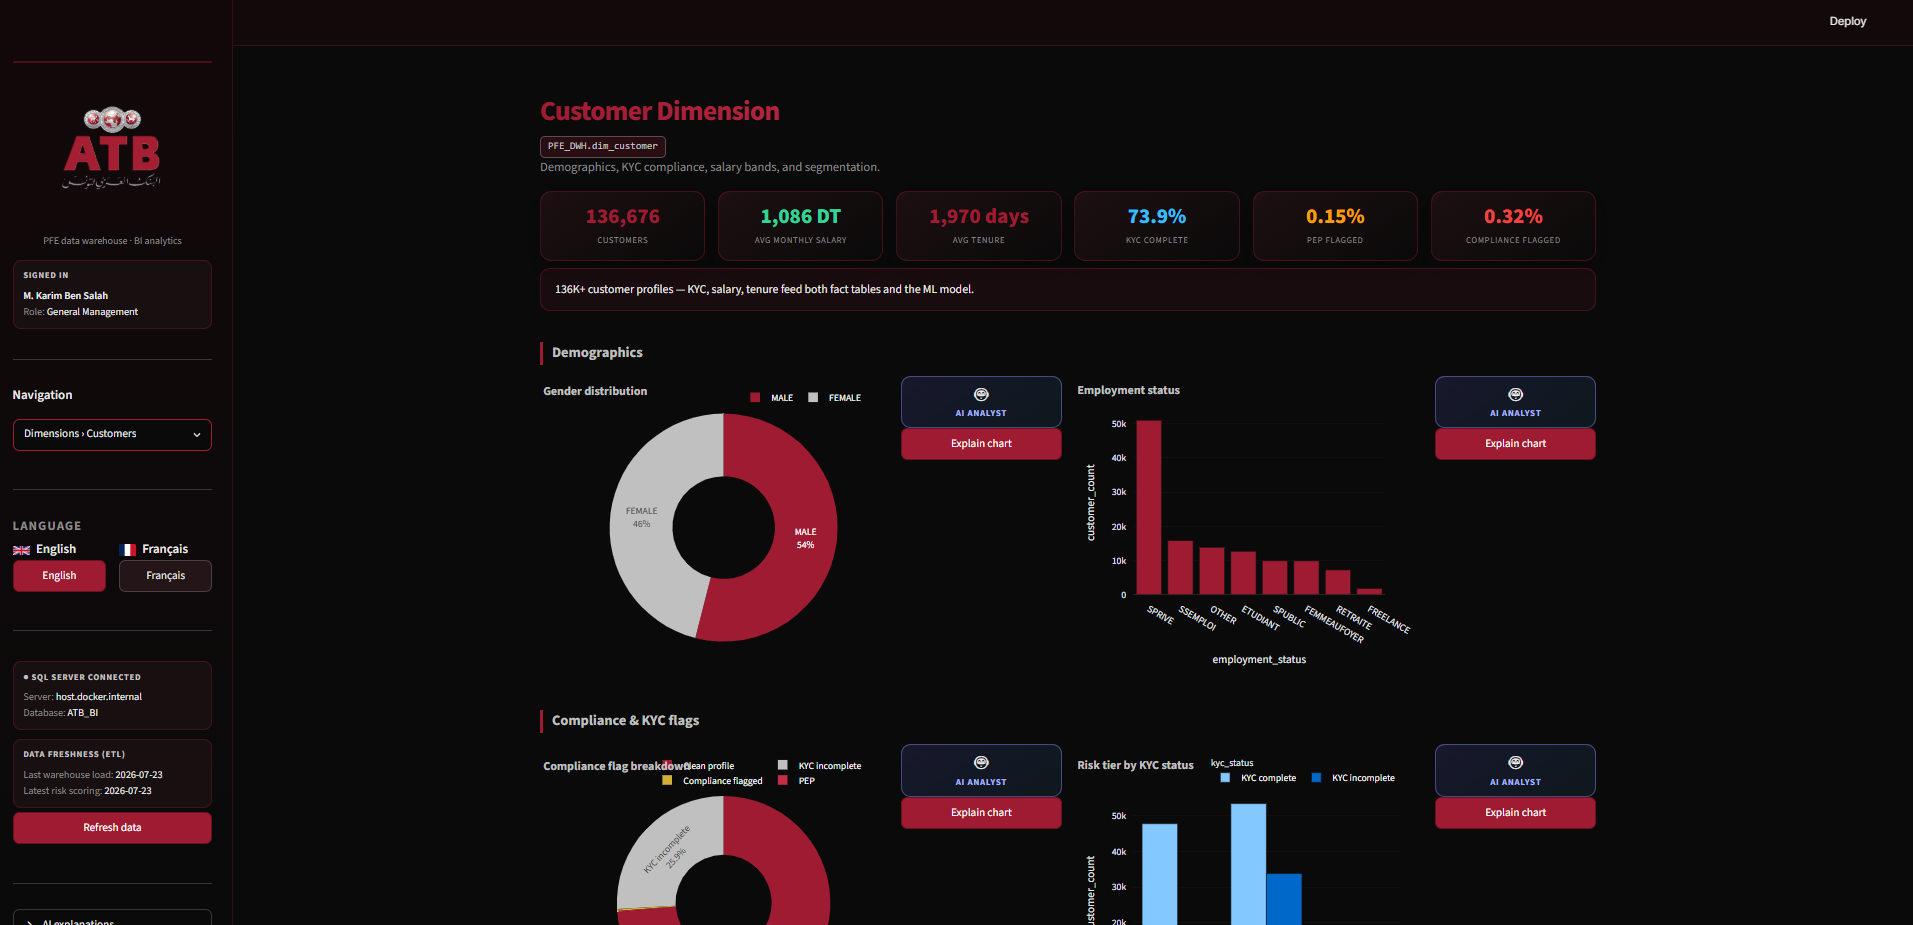
\includegraphics[width=0.88\textwidth]{figures/dash_dim_customer.png}
\caption{Customer dimension demographics, KYC compliance and salary context}
\label{fig:dash_dim_customer}
\end{figure}
\noindent Header KPIs summarise book size, salary, tenure and
regulatory flags (KYC 73.9\%, PEP 0.15\%). Gender and employment charts feed
both commercial steering and the demographic features later reused by ML.

\begin{figure}[H]
\centering
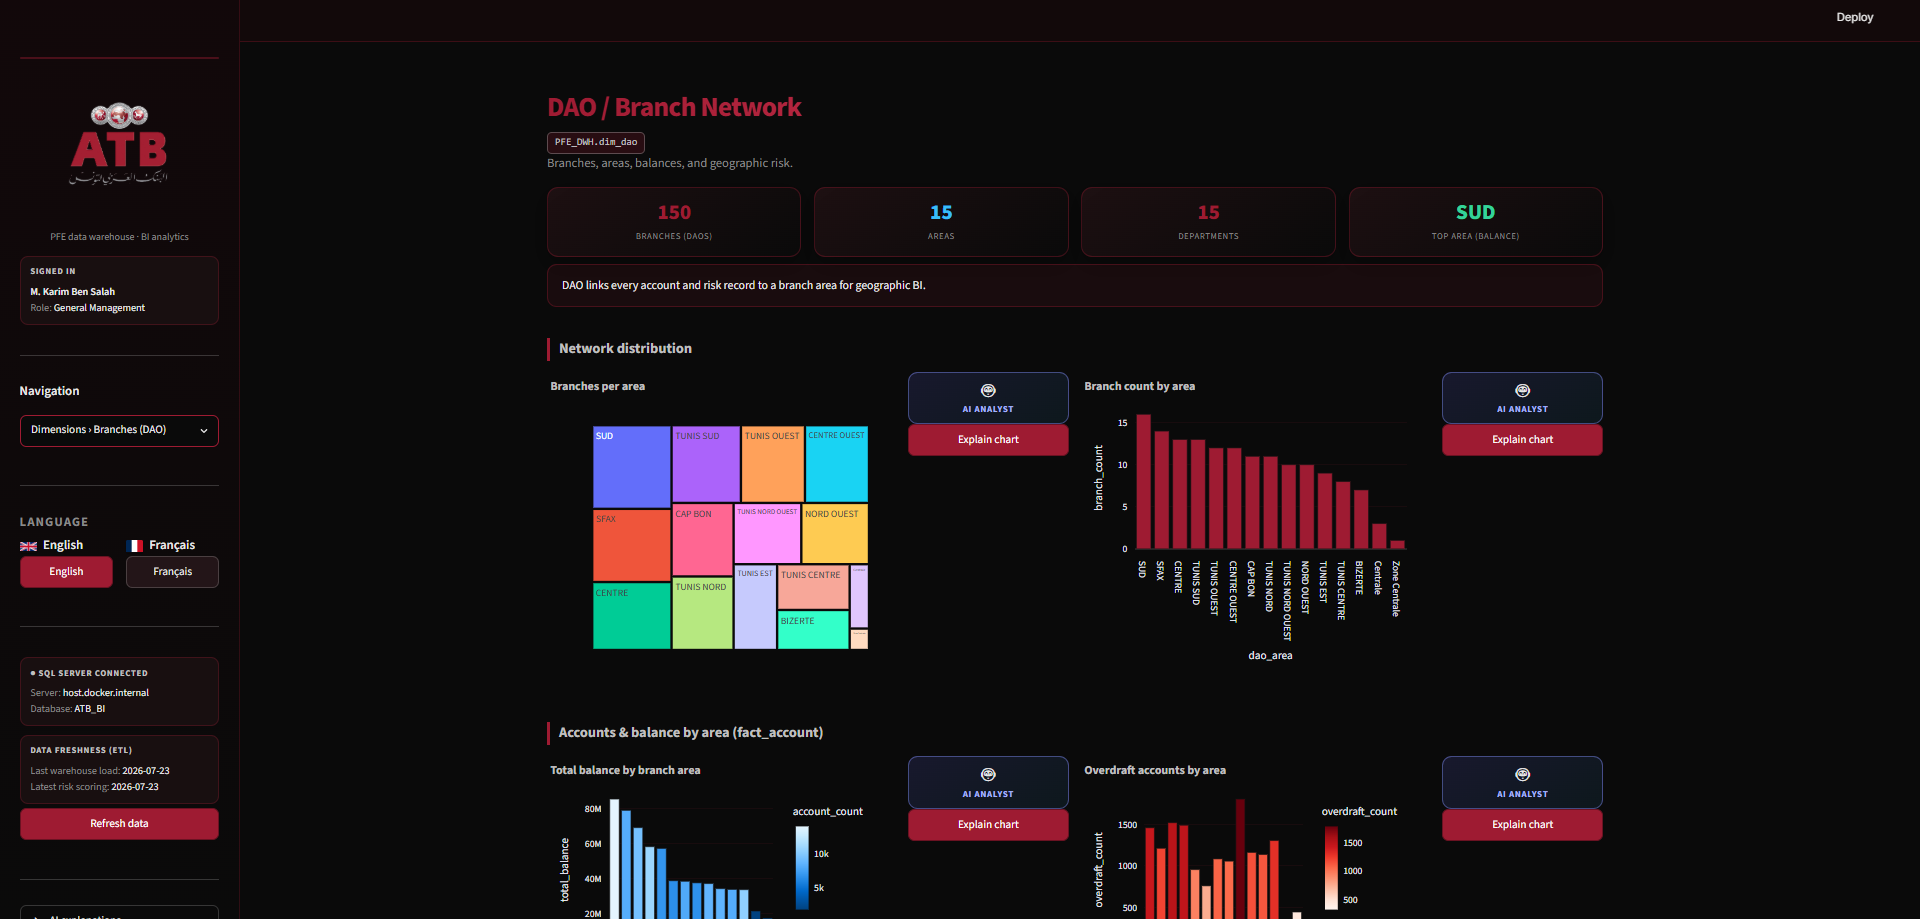
\includegraphics[width=0.88\textwidth]{figures/dash_dim_dao.png}
\caption{DAO / Branch Network area treemap, balance and overdraft by region}
\label{fig:dash_dim_dao}
\end{figure}
\noindent 150 DAOs across 15 areas: the treemap and branch-count
bars locate the network; balance and overdraft-by-area charts surface geographic
concentration the same page is DAO-scoped for Branch Managers (US~06).

\begin{figure}[H]
\centering
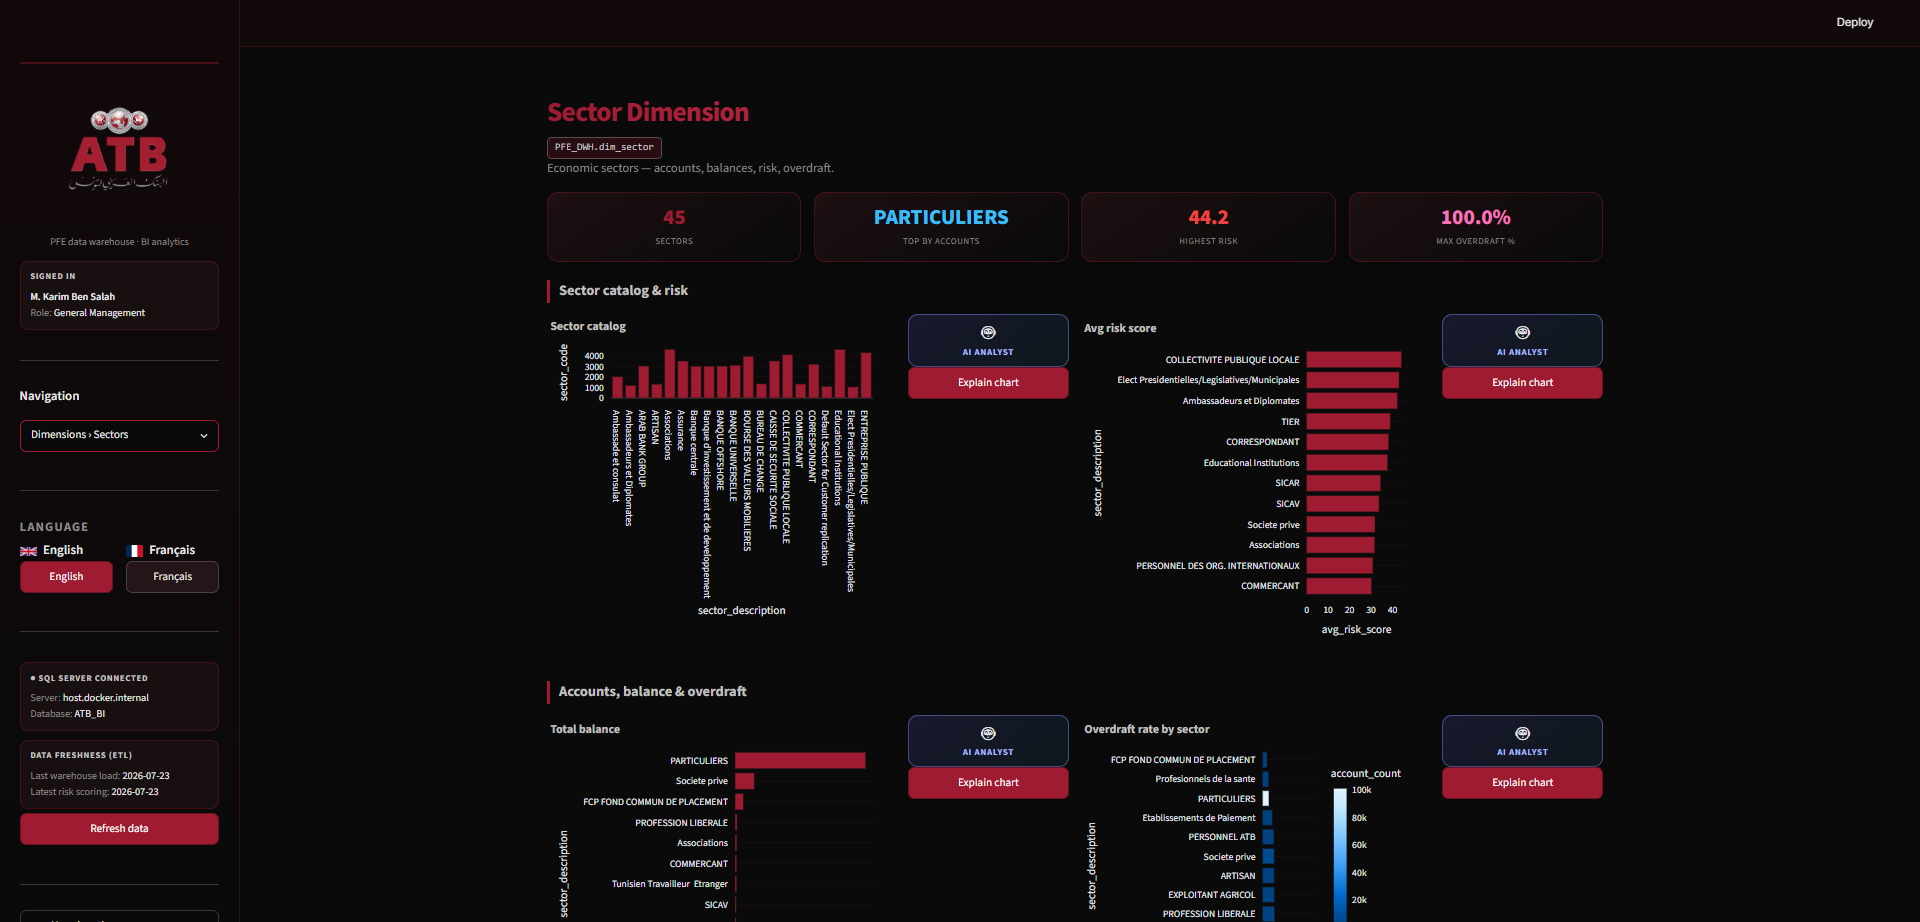
\includegraphics[width=0.88\textwidth]{figures/dash_dim_sector.png}
\caption{Sector dimension catalog, risk ranking, balance and overdraft rate}
\label{fig:dash_dim_sector}
\end{figure}
\noindent Forty-five economic sectors ranked by volume and
average risk; balance and overdraft-rate charts show which activities
concentrate solvency pressure.

\begin{figure}[H]
\centering
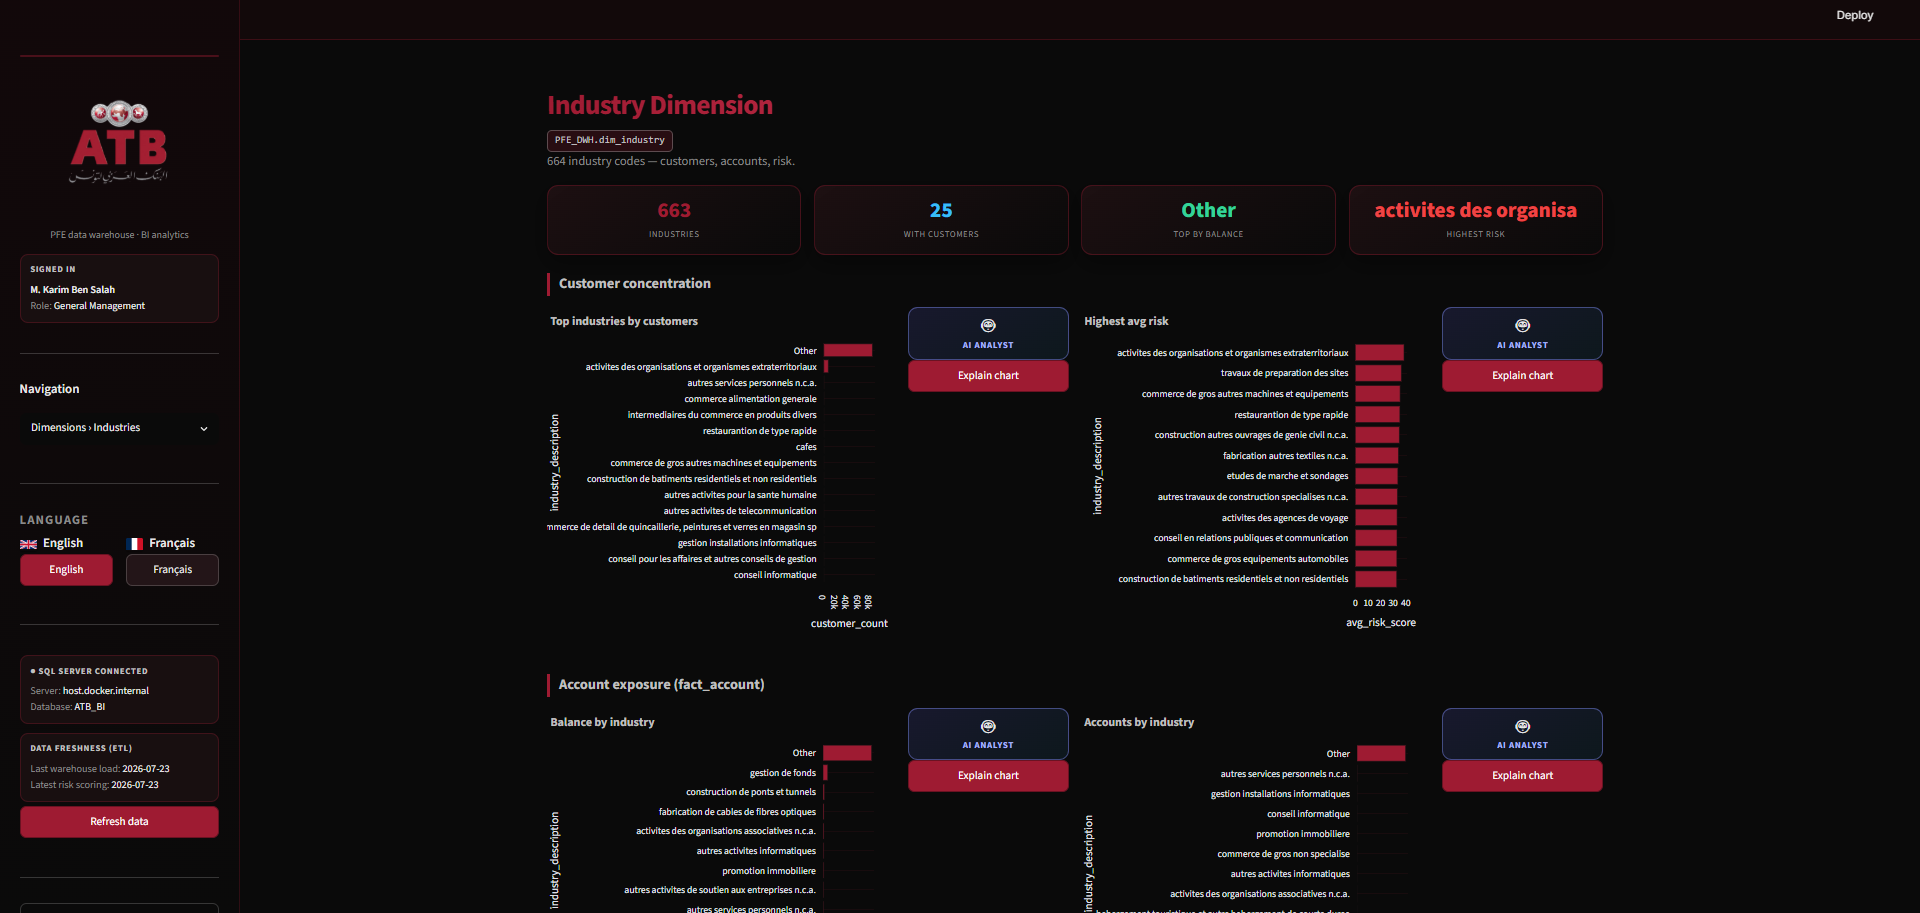
\includegraphics[width=0.88\textwidth]{figures/dash_dim_industry.png}
\caption{Industry dimension concentration bars and risk-vs-volume bubble}
\label{fig:dash_dim_industry}
\end{figure}
\noindent Industry pages drill one level finer than sectors:
concentration bars and risk-vs-volume bubbles isolate activity niches that
drive portfolio risk without drowning the committee in the full NACE catalog.

\begin{figure}[H]
\centering
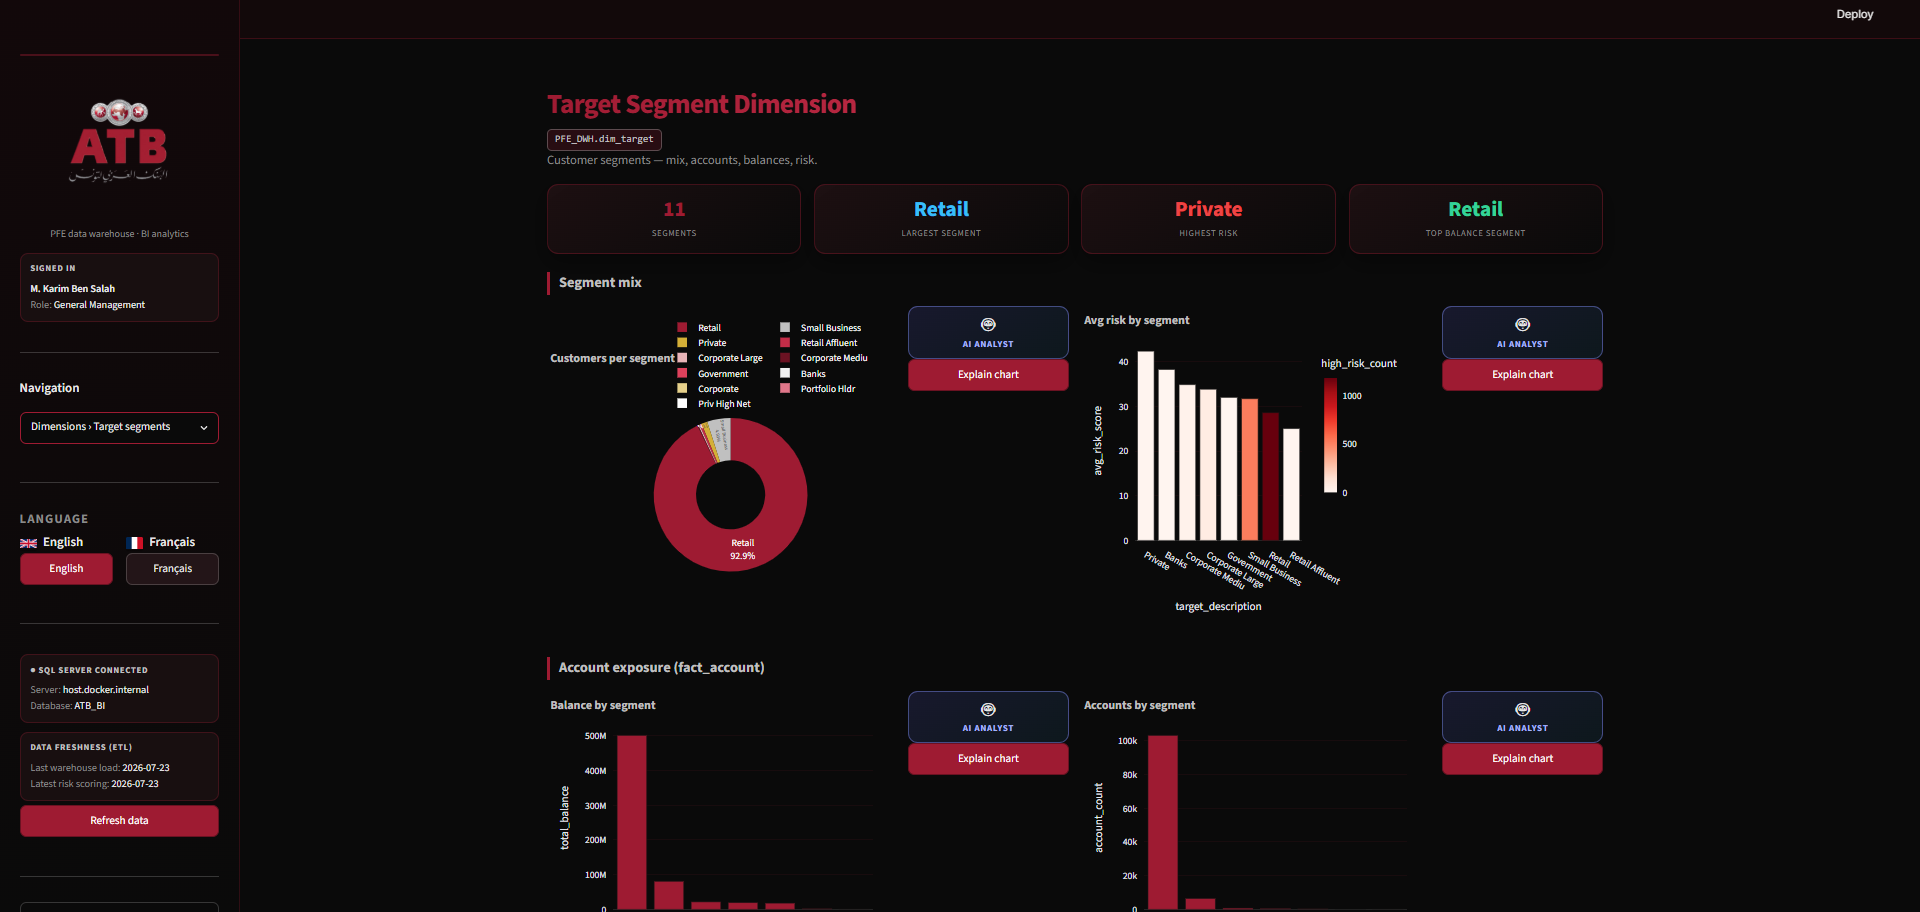
\includegraphics[width=0.88\textwidth]{figures/dash_dim_target.png}
\caption{Target segment dimension segment}
\label{fig:dash_dim_target}
\end{figure}
\noindent Commercial segments (retail, affluent, SME, corporate,
government) are compared on mix, average risk and balance so product and risk
teams share one vocabulary for book quality.

\begin{figure}[H]
\centering
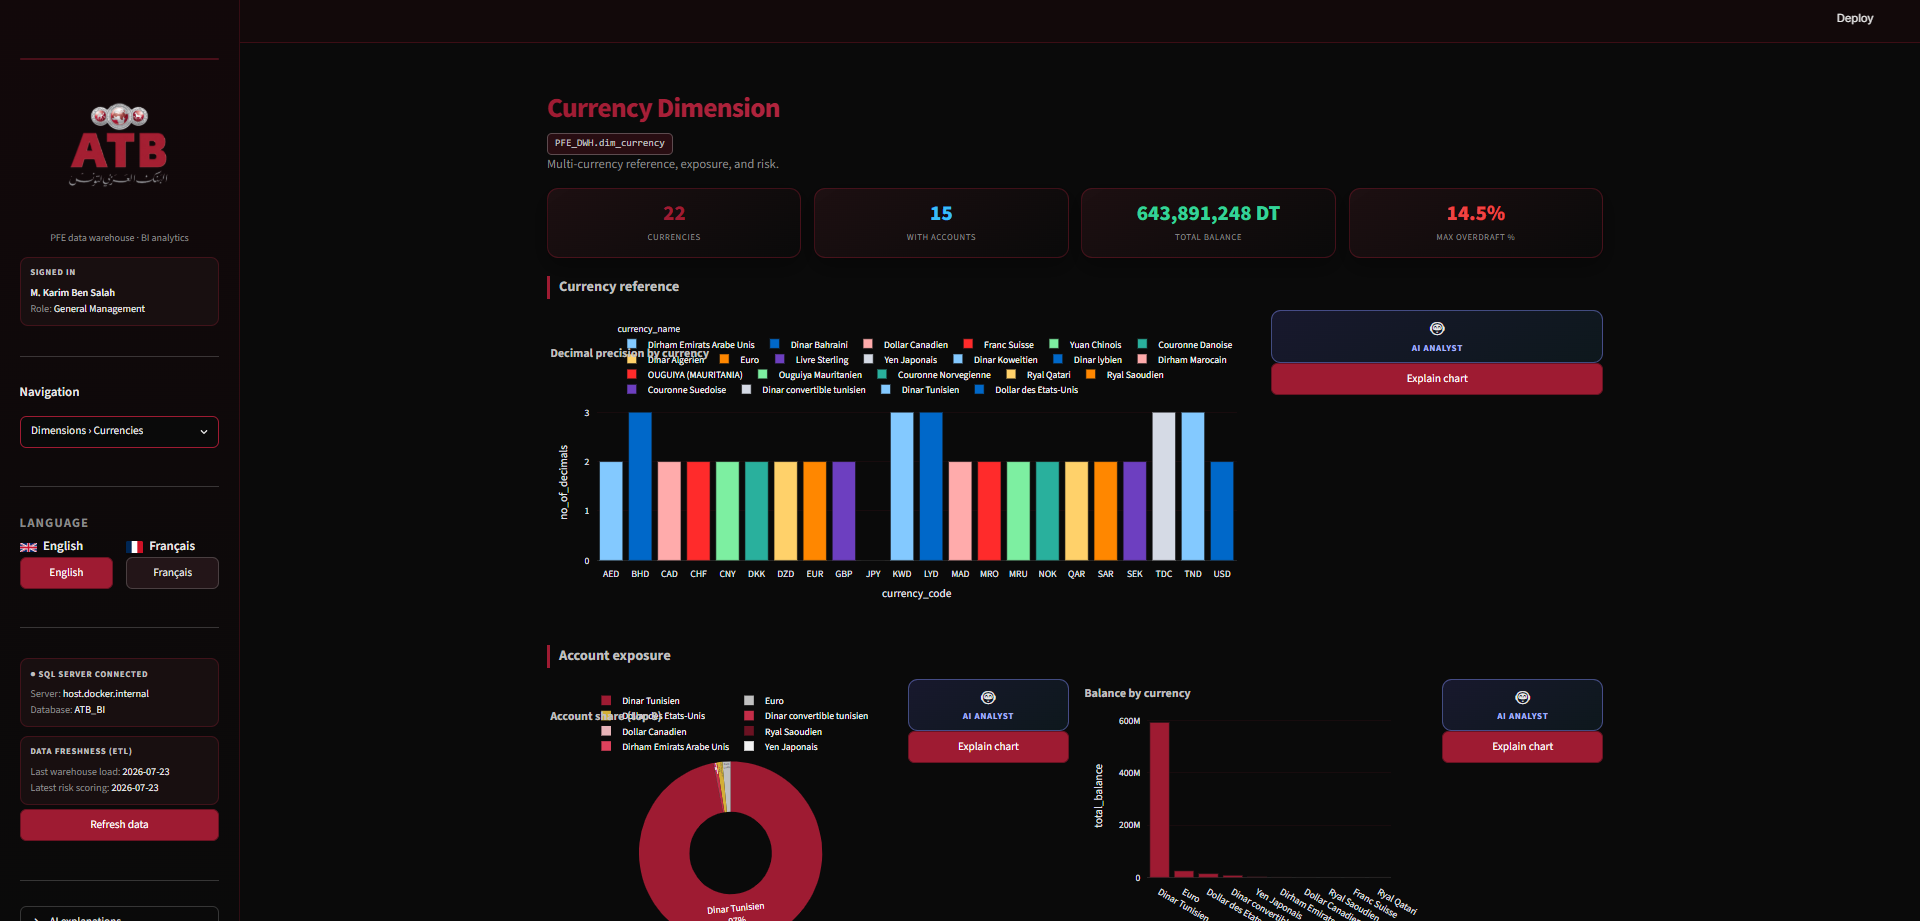
\includegraphics[width=0.88\textwidth]{figures/dash_dim_currency.png}
\caption{Currency dimension balance treemap}
\label{fig:dash_dim_currency}
\end{figure}
\noindent Multi-currency exposure, overdraft and risk by FX code
are summarised with a balance treemap essential when most balances sit in
TND but foreign-currency pockets still matter for ALM.

\begin{figure}[H]
\centering
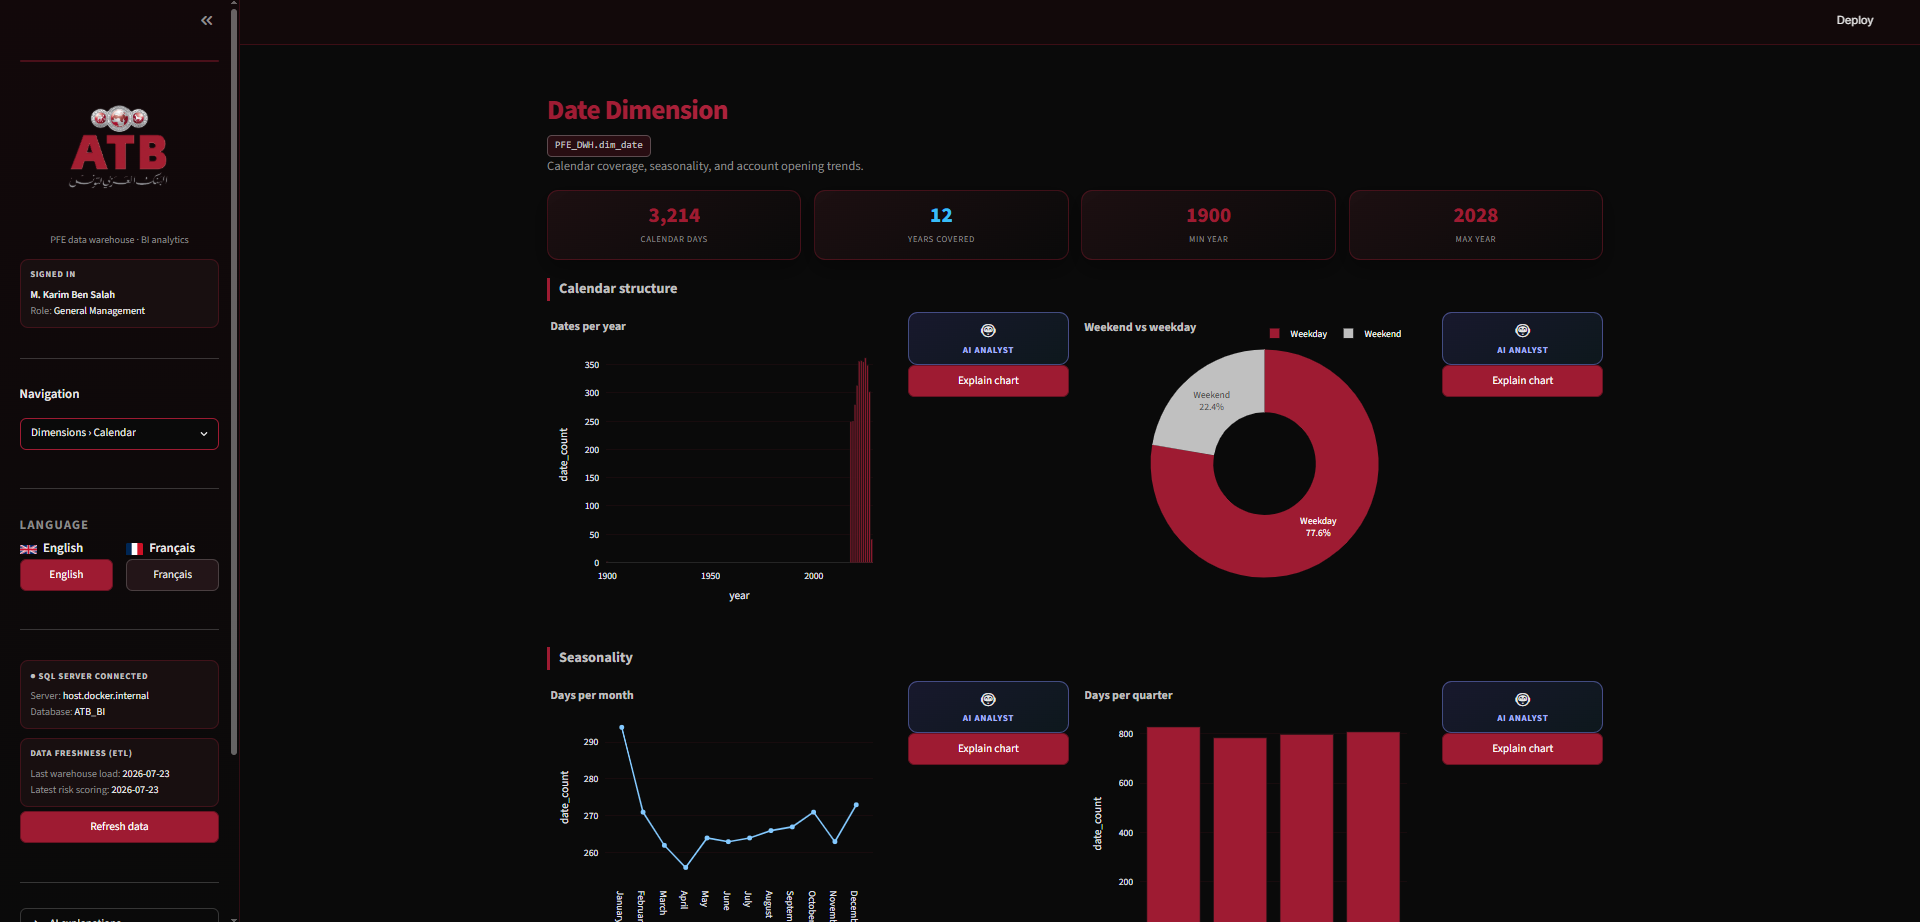
\includegraphics[width=0.88\textwidth]{figures/dash_dim_date.png}
\caption{Calendar dimension}
\label{fig:dash_dim_date}
\end{figure}
\noindent The date dimension turns openings and balances into a
vintage view: growth years, ageing cohorts and seasonality become visible
without exporting raw fact tables to Excel.

\paragraph{Extended KPI catalogue (facts + dimensions).}
Beyond the executive cards, the presentation layer surfaces the fuller set of
indicators prepared in Phase~2:

\begin{table}[H]
\centering
\caption{Extended KPI catalogue available across Streamlit pages}
\label{tab:extended_kpi_catalog}
\renewcommand{\arraystretch}{1.15}
\scriptsize
\begin{tabular}{|p{4.2cm}|p{4.0cm}|p{5.8cm}|}
\hline
\rowcolor{blue!15}
\textbf{KPI} & \textbf{Primary page(s)} & \textbf{Business reading} \\
\hline
Total customers / accounts & Overview, Customers & Book size \\
\hline
Total / average working balance & Overview, Accounts, DAO, Sector & Exposure and wallet size \\
\hline
Overdraft count \& rate & Overview, Accounts, DAO, Sector, Currency & Solvency pressure \\
\hline
Average GRS \& tier mix & Overview, Risk & Portfolio health \\
\hline
High-risk customer count / \% & Overview, Risk, Sector, Target & Priority follow-up mass \\
\hline
Mean CRI / FFS / BRS & Risk & Why the score is high \\
\hline
KYC completion \% & Overview, Compliance, Customers & Regulatory readiness \\
\hline
PEP \% \& flagged \% & Compliance, Customers & Enhanced due diligence load \\
\hline
Avg salary \& salary-band mix & Customers, Studies & Income fragility context \\
\hline
Avg tenure \& tenure bands & Customers, Studies & Relationship maturity \\
\hline
Employment / marital / gender mix & Customers & Demographic steering \\
\hline
Balance \& risk by DAO area & DAO, Comparison & Geographic concentration \\
\hline
Balance, risk, overdraft by sector/industry & Sector, Industry, Comparison & Activity concentration \\
\hline
Segment mix \& segment risk & Target & Commercial book quality \\
\hline
Openings \& balance by vintage year & Calendar & Growth and ageing of the book \\
\hline
FX exposure \& FX overdraft & Currency & Multi-currency risk \\
\hline
ETL freshness timestamp & Overview & Trust in the numbers \\
\hline
\end{tabular}
\end{table}

\subsection{Actionable Features and Sharing}
In line with GIMSI Phase~4 publication requirements, the interface is not limited
to passive charts:
\begin{itemize}
    \item \textbf{Visual alerting:} colour badges and alert inbox entries for
          incomplete KYC, PEP and high GRS;
    \item \textbf{Export / publication:} CSV downloads of filtered lists and
          executive PDF packs (disabled for read-only \texttt{AUDIT});
    \item \textbf{Manual cache refresh:} staff can invalidate TTL caches when an
          urgent recompute is required after an exceptional pipeline run.
\end{itemize}
\begin{figure}[H]
\centering
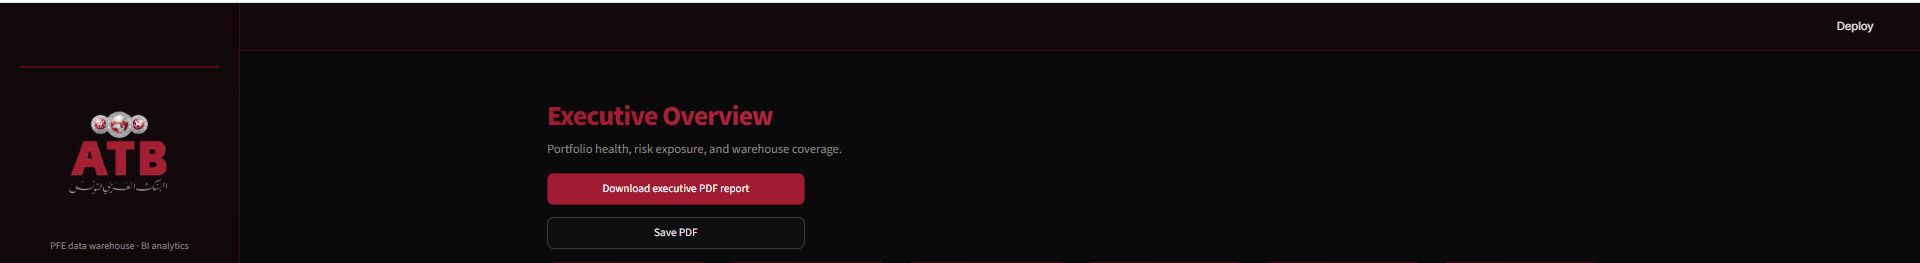
\includegraphics[width=0.75\textwidth]{figures/dash_export_csv.png}
\caption{CSV download button and exported filtered customer list}
\label{fig:dash_export_csv}
\end{figure}
\noindent Filtered risk or compliance lists leave the dashboard
as CSV for offline review disabled for the read-only \texttt{AUDIT} role.

\begin{figure}[H]
\centering
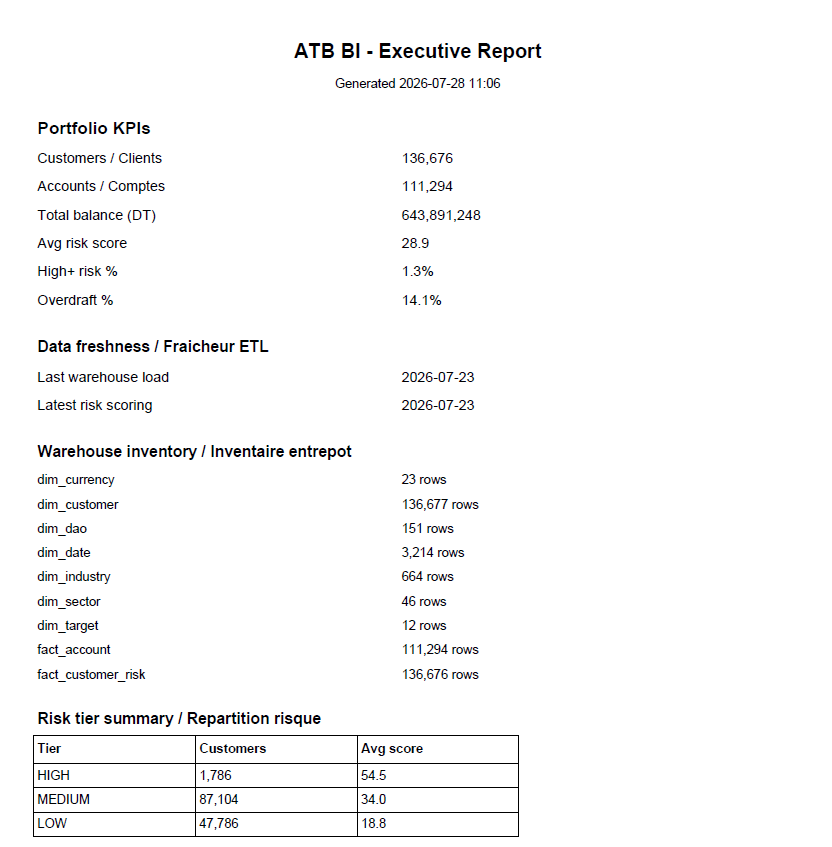
\includegraphics[width=0.75\textwidth]{figures/dash_export_pdf.png}
\caption{Executive PDF report preview}
\label{fig:dash_export_pdf}
\end{figure}
\noindent The executive PDF pack packages the overview KPIs and
key charts into a shareable artefact for committee circulation (GIMSI Phase~4
publication).

\begin{figure}[H]
\centering
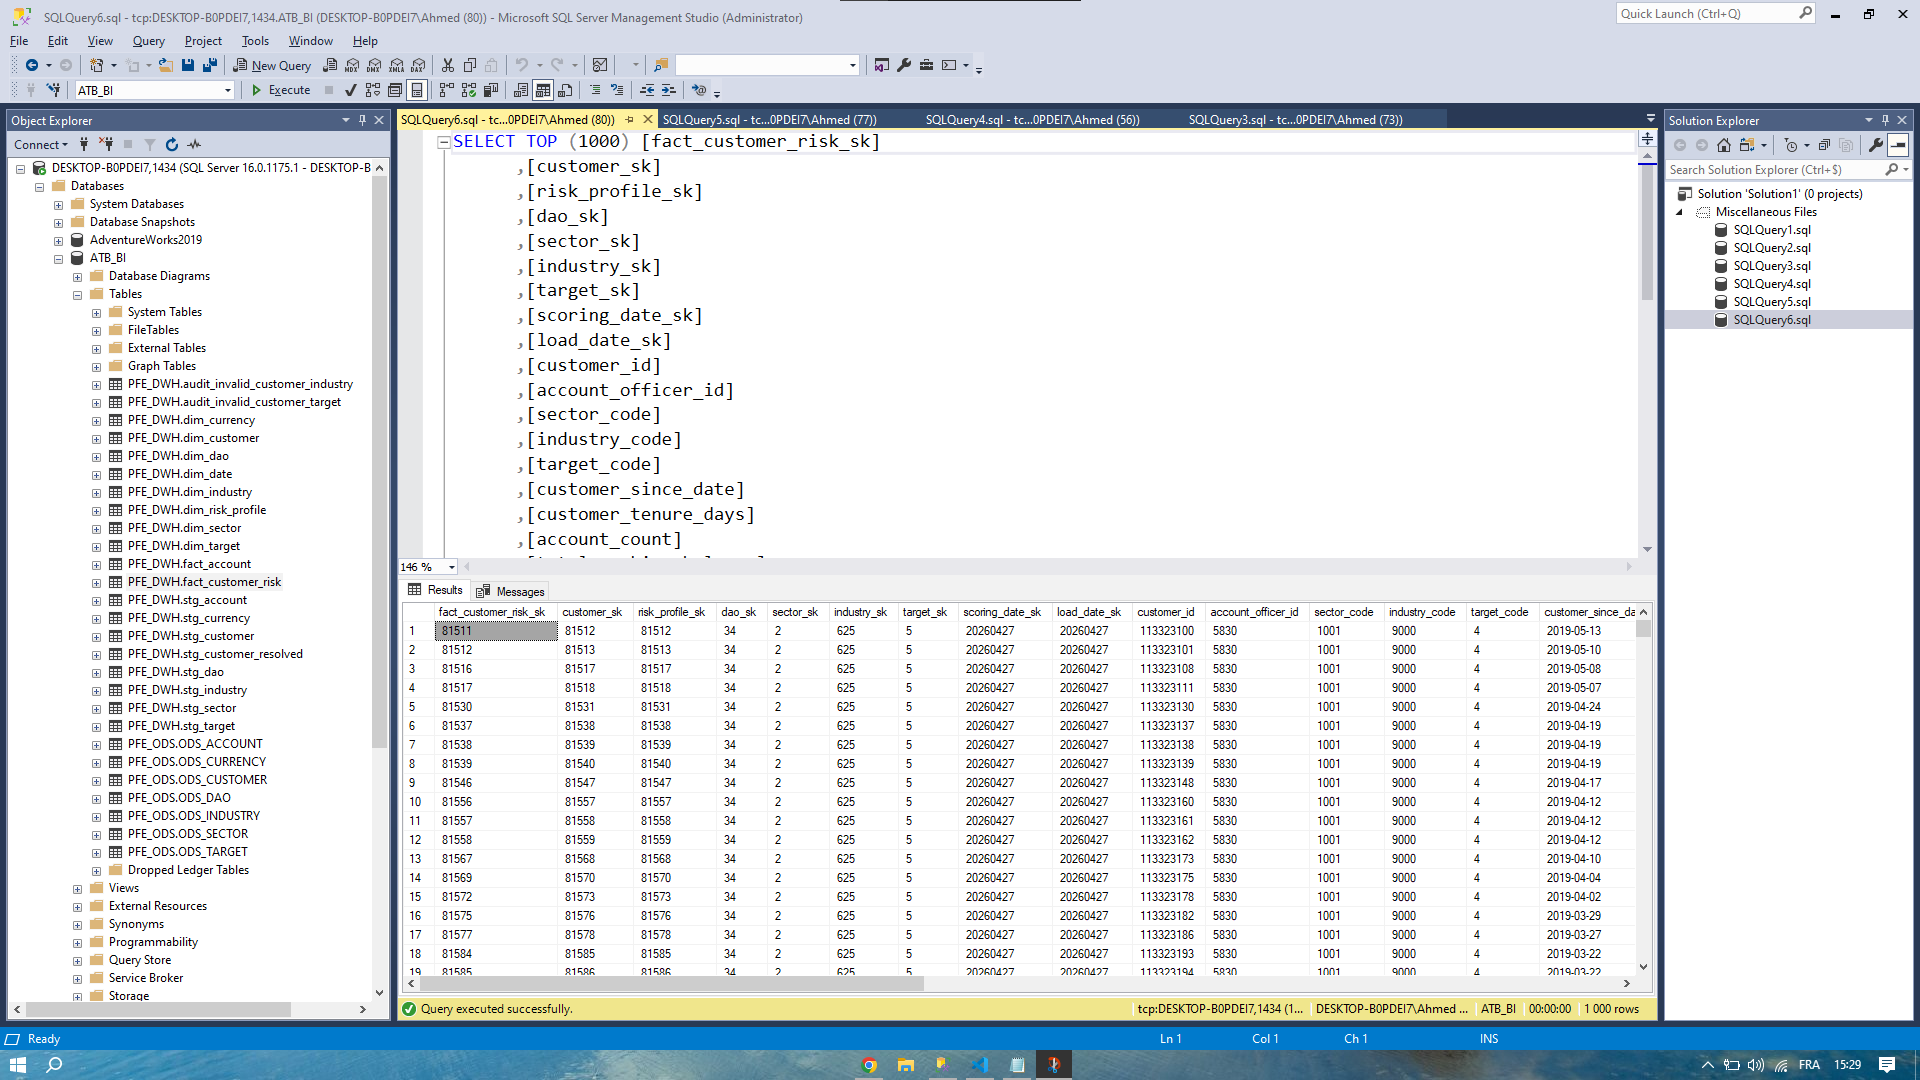
\includegraphics[width=0.88\textwidth]{figures/ssms_pfe_dwh.png}
\caption{SSMS Object Explorer --- \texttt{PFE\_DWH} dimensions and fact tables}
\label{fig:ssms_pfe_dwh}
\end{figure}
\noindent The constellation schema in SQL Server is the single
source of truth behind every Streamlit page shown above.

\begin{figure}[H]
\centering
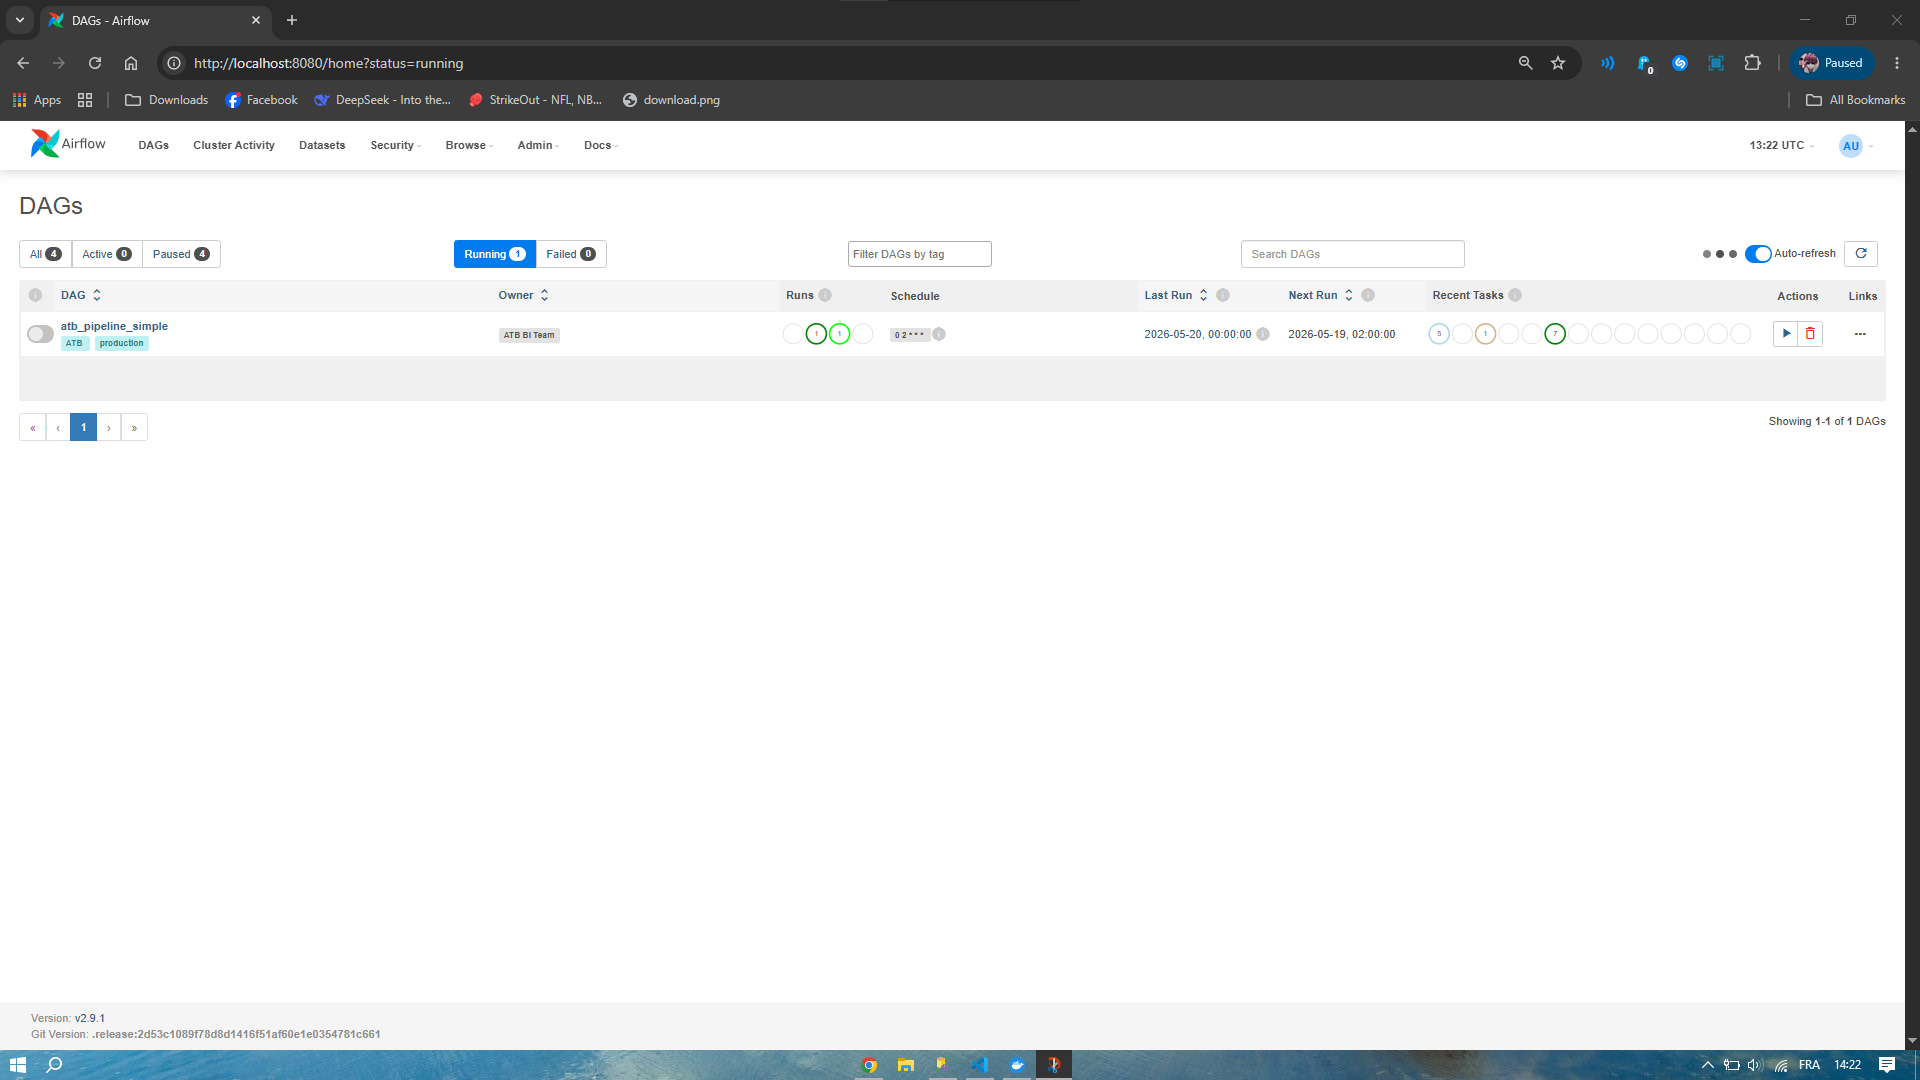
\includegraphics[width=0.88\textwidth]{figures/airflow_master_dag.png}
\caption{Airflow DAG graph view of Master pipeline}
\label{fig:airflow_master_dag}
\end{figure}
\noindent Nightly orchestration (ingestion $\rightarrow$ dbt
$\rightarrow$ quality $\rightarrow$ optional ML) keeps the warehouse --- and
therefore the dashboard TTL caches --- aligned with source extracts.

%======================================================================
\section{Phase 4: Evaluation and Continuous Improvement}
\label{sec:gimsi_phase4}
%======================================================================
The last GIMSI phase marks the completion of the decision cycle. Beyond visual
restitution, it evaluates the tool under real conditions and plans continuous
improvements. A decision dashboard loses value if displayed information is stale;
yet querying SQL Server on every click would overload the server and degrade
latency.

\subsection{Refresh Mechanism (Near Real Time)}
We synchronised Streamlit with the Airflow nightly rebuild using
\texttt{@st.cache\_data(ttl=...)} in the data-access layer.

\begin{itemize}
    \item Executive KPI loaders typically use $\mathrm{TTL}=300$~s (5~minutes);
    \item distribution loaders use $\mathrm{TTL}=180$~s (3~minutes);
    \item AI explanations use $\mathrm{TTL}=3600$~s (stable textual tips).
\end{itemize}

\paragraph{Production data life cycle.}
\begin{enumerate}
    \item \textbf{Nightly rebuild (02:00 UTC):} Airbyte + dbt + quality checks
          refresh \texttt{PFE\_DWH}.
    \item \textbf{First morning click:} Streamlit loads fresh warehouse rows into
          cache.
    \item \textbf{Interactive service:} subsequent filters/pages are served from
          memory until TTL expiry.
    \item \textbf{Manual refresh:} operators may clear cache after an exceptional
          recompute.
\end{enumerate}

\begin{figure}[H]
\centering
\begin{tikzpicture}[
  font=\scriptsize,
  step/.style={rectangle, rounded corners=2pt, draw=#1, fill=#1!12, thick,
               align=center, minimum width=2.55cm, minimum height=1.15cm},
  arr/.style={->, thick}
]
  \node[step=teal!70!black] (a) {Airflow\\02:00 UTC};
  \node[step=blue!70!black, right=0.4cm of a] (b) {dbt build\\+ tests};
  \node[step=violet!70!black, right=0.4cm of b] (c) {\texttt{PFE\_DWH}\\fresh facts};
  \node[step=orange!80!black, right=0.4cm of c] (d) {Streamlit\\TTL cache};
  \draw[arr] (a) -- (b);
  \draw[arr] (b) -- (c);
  \draw[arr] (c) -- (d);
\end{tikzpicture}
\caption{Freshness chain --- nightly Airflow rebuild to Streamlit TTL cache}
\label{fig:freshness_chain}
\end{figure}

\subsection{Perspectives for Continuous Improvement}
GIMSI Phase~4 also implies that the decision system must not remain static:
\begin{itemize}
    \item \textbf{Evolutionary KPI adjustment:} new regulatory fields can be added as
          point rules in \texttt{int\_customer\_risk\_score.sql} without redesigning
          the constellation.
    \item \textbf{Periodic technical audits:} monitor ELT duration, index health,
          parse rates and tier-distribution drift.
    \item \textbf{Weight governance:} re-run sensitivity analysis when the risk
          committee changes priorities.
    \item \textbf{Predictive extension:} Release~3 replaces purely descriptive
          steering with supervised models and MLflow tracking on the same warehouse
          features.
\end{itemize}

%======================================================================
\section{Conclusion}
\label{sec:release2_conclusion}
%======================================================================
%----------------------------------------------------------------------
% SCREENSHOT CHECKLIST (commented — capture these, then uncomment includegraphics)
% Save under report/figures/ with the exact names below, then replace the
% nearby %% TODO_SCREENSHOT lines with:
%   \begin{figure}[H]\centering\includegraphics[width=0.85\textwidth]{figures/NAME.png}
%   \caption{...}\label{fig:...}\end{figure}
%
% INGESTION
%   [ ] airbyte_docker_ui.png
%   [ ] airbyte_github_source.png
%   [ ] airbyte_connections_list.png
%   [ ] airbyte_sync_success.png
%   [ ] github_raw_csv.png
% CLEANING
%   [ ] stg_customer_sql.png
%   [ ] dbt_test_pass.png
%   [ ] ods_vs_stg_compare.png
% DASHBOARD CORE
%   [ ] dash_overview_kpis.png
%   [ ] dash_studies.png
%   [ ] dash_compliance.png
%   [ ] dash_alert_inbox.png
%   [ ] dash_risk_pillars.png
%   [ ] dash_accounts.png
%   [ ] dash_rbac_branch.png
%   [ ] dash_ai_explain.png
% DIMENSION PAGES
%   [ ] dash_dim_customer.png
%   [ ] dash_dim_dao.png
%   [ ] dash_dim_sector.png
%   [ ] dash_dim_industry.png
%   [ ] dash_dim_target.png
%   [ ] dash_dim_currency.png
%   [ ] dash_dim_date.png
% EXPORT / OPS
%   [ ] dash_export_csv.png
%   [ ] dash_export_pdf.png
%   [ ] ssms_pfe_dwh.png
%   [ ] airflow_master_dag.png
%----------------------------------------------------------------------
This second iteration (Release~2) transformed raw operational extracts into a
genuine decision-support system. Rigorous application of GIMSI guaranteed an
optimal four-layer structure: from Airbyte acquisition and dbt ELT through a
robust SQL Server constellation warehouse to interactive Streamlit restitution.

At the heart of the architecture, the three-pillar weighted baseline
($40\%$ compliance / $35\%$ financial / $25\%$ behavioural) proved effective and
explainable. Feature-driver analysis empirically validated the business choices by
confirming the predominance of KYC quality, salary/balance pressure and tenure
signals. Central Management, Compliance and Branch Managers now share a visual,
actionable and role-safe cockpit built on $281{,}960$ referentially clean fact
rows.

However, although this heuristic approach offers very satisfactory descriptive
performance, it remains static relative to evolving customer behaviour. The final
project stage (Release~3) will therefore complement the deterministic scoring
engine with Machine Learning models, in order to make risk anticipation
predictive and self-adaptive while reusing the warehouse, KPIs and dashboard
shell already validated here.
